%%%%%%%% FireGate (formerly Tripwire), version 4.2 (clean): label-free forgetting certificates for continual RL fine-tuning %%%%%%%%
% CLEAN VERSION (Nov 1): main_v4.tex without the plan appendix. The main text ends at the top of page nine (the ICML
% submission limit is eight, the camera-ready limit nine); everything else is in the appendix. Results are read from
% paper/v2_results/ (bash slurm/plan.sh collect; python scripts/table_style.py paper/v2_results restyles the tables).
% Version 3.5 (Nov 2, PLAN_PAPER3.md): v3.4 with the protect gate's remedy (step p3.8, v3_results_20261102_0219).
% Version 4.9 (Nov 4): Appendix K results in the main text, Table 1's fresh-Dolly bound, scoped wording, nine new
% references.
% Version 4.5 (Nov 3): p3.9, p3.12, p3.14, p3.15 results (Appendix K, Section 6) and the theory pass (Corollary 4.2,
% Propositions A.2-A.4, Remark A.1); appendix in small type to stay within 50 pages.
% Version 4.4 (Nov 2), Overleaf build: tab:main7 and tab:main5 inlined so their references resolve; text unchanged.
% Version 4.4 (Nov 2): p3.10 and p3.11 results (score classes at delta/4 with the region, second-round forms) in 6.4-6.6 and Appendix G.3, I.
% Version 4.2 (Nov 2): v4.1 with SQuAD 2.0 alone in Table 3 (Concise in Appendix J) and the Fisher detail in Appendix H.
% Version 4.1 (Nov 2): version 4 within 50 pages in all (appendix packed, repeated text removed).
% Version 4 (Nov 2): the main text of version 3.5 restructured as a research paper (problem, certificate, its
% price, method, evidence); every result of version 3.5 is kept, in the main text or the appendix.
\documentclass{article}

\usepackage{microtype}
\usepackage{graphicx}
\usepackage{subcaption}
\usepackage{booktabs}
\usepackage{array}
\usepackage{multirow}
\usepackage{hyperref}
\newcommand{\theHalgorithm}{\arabic{algorithm}}

% Preprint: names, institute and email shown. For the blind submission use \usepackage{icml2026}.
\usepackage[preprint]{icml2026}
\newcommand{\authoremail}{\mbox{manwar@iastate.edu}}% first author's email
\hyphenation{TriviaQA}
\makeatletter
\ificmlshowauthors % preprint: no affiliation marks or footnote; the institute and emails sit under the names
  \renewcommand{\@pa}[1]{}
  \renewcommand{\icmlaffiliation}[2]{}
  \renewcommand{\printAffiliationsAndNotice}[1]{\global\icml@noticeprintedtrue
    {\let\thefootnote\relax\footnotetext{\hspace*{-\footnotesep}\Notice@String}}}
\fi
\makeatother

\usepackage{amsmath}
\usepackage{amssymb}
\usepackage{mathtools}
\usepackage{amsthm}
\usepackage{xcolor}
\usepackage{tikz}
\usetikzlibrary{arrows.meta,positioning,fit,calc,backgrounds}
\usepackage{pgfplots}
\pgfplotsset{compat=1.16}
\usepgfplotslibrary{groupplots}
\usepackage{placeins}
\usepackage[capitalize,noabbrev]{cleveref}

\theoremstyle{plain}
\newtheorem{theorem}{Theorem}[section]
\newtheorem{proposition}[theorem]{Proposition}
\newtheorem{lemma}[theorem]{Lemma}
\newtheorem{corollary}[theorem]{Corollary}
\theoremstyle{definition}
\newtheorem{definition}[theorem]{Definition}
\newtheorem{assumption}[theorem]{Assumption}
\theoremstyle{remark}
\newtheorem{remark}[theorem]{Remark}

% ---------- macros ----------
\newcommand{\R}{\mathbb{R}}
\newcommand{\E}{\mathbb{E}}
\newcommand{\TV}{\mathrm{TV}}
\newcommand{\KL}{\mathrm{KL}}
\newcommand{\kl}{\mathrm{kl}}
\newcommand{\Dref}{D_{\mathrm{ref}}}
\newcommand{\Dnew}{D_{\mathrm{new}}}
\newcommand{\pold}{\pi_{\mathrm{old}}}
\newcommand{\pnew}{\pi_{\mathrm{new}}}
\newcommand{\Fire}{\mathsf{F}}
\renewcommand{\lg}{\ell_{\mathrm{g}}}
\newcommand{\ind}{\mathbf{1}}
\newcommand{\method}{\textsc{FireGate}}
\newcommand{\methodp}{\textsc{FireGate}-prompt}
\newcommand{\methoda}{\textsc{FireGate}-anytime}
\newcommand{\pending}[1]{\textcolor{blue!60!black}{[#1]}}
\DeclareMathOperator*{\argmax}{arg\,max}

% ---------- results (written by bash slurm/plan.sh collect into v2_results/) ----------
\newcommand{\resdir}{latex_v2_results}% only the result files this paper uses (copied from v2_results)
\newcommand{\Sdir}{\resdir/v2_stream_q15/results}
\newcommand{\Odir}{\resdir/v2_overlap_q15/results}
\newcommand{\Oana}{\resdir/v2_overlap_q15/analysis}
\newcommand{\Idir}{\resdir/v2_ladder_ifc_q15/results}
\newcommand{\Cdir}{\resdir/v2_ladder_concise_q15/results}
\newcommand{\SSdir}{\resdir/v2_stream_q7/results}
\newcommand{\OSdir}{\resdir/v2_overlap_q7/results}
\newcommand{\OOdir}{\resdir/v2_overlap_olmo7/results}
\newcommand{\ISdir}{\resdir/v2_ladder_ifc_q7/results}
\newcommand{\FSdir}{\resdir/v2_stream5_q15/results}
\newcommand{\OVdir}{\resdir/overview}
\newcommand{\placeholder}[1]{\begin{center}\fbox{\parbox[c][1.6cm][c]{0.9\linewidth}{\centering\small
  \textcolor{blue!60!black}{#1}}}\end{center}}
\newcommand{\inputor}[2]{\IfFileExists{#1}{\input{#1}}{\placeholder{#2}}}
\IfFileExists{\Sdir/numbers.tex}{\input{\Sdir/numbers.tex}}{}
\IfFileExists{\Odir/overlap_numbers.tex}{\input{\Odir/overlap_numbers.tex}}{}
\IfFileExists{\Idir/overlap_ifc_numbers.tex}{\input{\Idir/overlap_ifc_numbers.tex}}{}
\IfFileExists{\Cdir/overlap_concise_numbers.tex}{\input{\Cdir/overlap_concise_numbers.tex}}{}
\IfFileExists{\Sdir/extra_numbers.tex}{\input{\Sdir/extra_numbers.tex}}{}
\IfFileExists{\OSdir/overlap_seven_numbers.tex}{\input{\OSdir/overlap_seven_numbers.tex}}{}
\IfFileExists{\OOdir/overlap_olmo_numbers.tex}{\input{\OOdir/overlap_olmo_numbers.tex}}{}
\IfFileExists{\ISdir/overlap_ifcseven_numbers.tex}{\input{\ISdir/overlap_ifcseven_numbers.tex}}{}
\newcommand{\CXdir}{\resdir/v2_ladder_concisectx_q15/results}
\IfFileExists{\CXdir/overlap_concisectx_numbers.tex}{\input{\CXdir/overlap_concisectx_numbers.tex}}{}
% review analyses (scripts/switch_analyses.py, review_analyses.py, judge_agreement.py): \an<Exp>..., \rv<Exp>..., \ja...
\newcommand{\inputif}[1]{\IfFileExists{#1}{\input{#1}}{}}
\inputif{\resdir/v2_overlap_q15/switch/analyses/analyses_numbers.tex}
\inputif{\resdir/v2_overlap_q15/switch/review/review_numbers.tex}
\inputif{\resdir/v2_ladder_ifc_q15/switch/analyses/analyses_numbers.tex}
\inputif{\resdir/v2_ladder_ifc_q15/switch/review/review_numbers.tex}
\inputif{\resdir/v2_ladder_concisectx_q15/switch/analyses/analyses_numbers.tex}
\inputif{\resdir/v2_ladder_concisectx_q15/switch/review/review_numbers.tex}
\inputif{\resdir/v2_overlap_q7/switch/analyses/analyses_numbers.tex}
\inputif{\resdir/v2_overlap_q7/switch/review/review_numbers.tex}
\inputif{\resdir/v2_overlap_olmo7/switch/analyses/analyses_numbers.tex}
\inputif{\resdir/v2_overlap_olmo7/switch/review/review_numbers.tex}
% certified switches and gate variants of every experiment (python scripts/make_switch_overview.py):
% \ovw<Exp><Family><Variant><Metric> and \ovg<Exp><Variant><Pool>
\IfFileExists{\OVdir/overview_macros.tex}{\input{\OVdir/overview_macros.tex}}{}
% review round 3 (Oct 29): two-sided sensitivity, covariance term, stream budget (python scripts/review2_analyses.py
% --aggregate, \rvbAll...), serving cost (scripts/latency_bench.py, \latSmall... / \latSeven...)
\inputif{\OVdir/review2/review2_numbers.tex}
% held-out and calibration sample sizes of a certificate (python scripts/cp_sample_size.py): \cpN..., \cpCalib...
\inputif{\OVdir/cp_sample_size_numbers.tex}
% drift under other decoding rules (bash slurm/plan.sh decode-collect): \dec...
\inputif{\resdir/decode/decode_numbers.tex}
\providecommand{\decNonfired}{--}\providecommand{\decNonfiredChecked}{--}\providecommand{\decGatedChgMax}{--}
\providecommand{\decNqSeqLbMin}{--}\providecommand{\decNqSeqLbMax}{--}
\providecommand{\cpNTwoFiveTyp}{--}\providecommand{\cpNTwoThreeTyp}{--}\providecommand{\cpCalibOne}{--}
\providecommand{\cpNqObserved}{--}\providecommand{\cpNqAtSixteen}{--}
\inputif{\resdir/latency/latency_small_numbers.tex}
\inputif{\resdir/latency/latency_seven_numbers.tex}
\providecommand{\ovwPredBlN}{--}\providecommand{\ovwPredBlMae}{--}\providecommand{\ovwPredBlMax}{--}
\providecommand{\ovwPredBlGain}{--}\providecommand{\ovwPredOneN}{--}\providecommand{\ovwCpDollyMax}{--}
\providecommand{\ovwCpDollyMaxStream}{--}
\providecommand{\rvbAllCovN}{--}\providecommand{\rvbAllCovZero}{--}\providecommand{\rvbAllCovErrMax}{--}
\providecommand{\rvbNqBeta}{--}\providecommand{\rvbNqDeployed}{--}\providecommand{\rvbNqRandomMean}{--}
\providecommand{\rvbNqWorst}{--}\providecommand{\rvbNqSolvedFirst}{--}\providecommand{\rvbNqFeatureAdv}{--}
\providecommand{\rvbNqRtwo}{--}\providecommand{\rvbNqPredEval}{--}\providecommand{\rvbAllConsRtwoMax}{--}
\providecommand{\rvbAllSensPowerMin}{--}\providecommand{\rvbAllSensPowerMax}{--}\providecommand{\rvbAllSensJbMax}{--}
\providecommand{\rvbAllSensProbeJbMax}{--}
\providecommand{\rvbAllBudStages}{--}\providecommand{\rvbAllBudHaveMin}{--}\providecommand{\rvbAllBudFiveCert}{--}
\providecommand{\rvbAllBudTenCert}{--}\providecommand{\rvbAllBudTenNeed}{--}\providecommand{\rvbAllBudTwentyNeed}{--}
\providecommand{\rvbAllBudTenStream}{--}
\providecommand{\latSmallPromptOneRel}{--}\providecommand{\latSmallPromptTwentyRel}{--}
\providecommand{\latSmallPromptTwentyRelOne}{--}\providecommand{\latSmallPromptTwentyPeak}{--}
\providecommand{\latSmallBasePeak}{--}\providecommand{\latSmallGateShare}{--}\providecommand{\latSmallSwitchRel}{--}
\providecommand{\latSmallSwitchPeak}{--}\providecommand{\latSmallAnytimeTwentyRel}{--}
\providecommand{\latSevenPromptTwentyRel}{--}\providecommand{\latSevenGateShare}{--}
% the 7B stream files use the same macro names as the 1.5B ones: they are read under a prefix, \sev{resAvgSeq}
% is the 7B value of \resAvgSeq (-- if the file or the value is missing)
\makeatletter
\def\tw@inputprefixed#1#2{\begingroup
  \def\newcommand##1##2{\expandafter\xdef\csname #1\expandafter\@gobble\string##1\endcsname{\unexpanded{##2}}}%
  \input{#2}\endgroup}
\def\tw@inputrelabel#1#2{\begingroup\let\origlabel\label\def\label##1{\origlabel{#1}}\input{#2}\endgroup}
\newcommand{\inputprefixed}[2]{\IfFileExists{#2}{\tw@inputprefixed{#1}{#2}}{}}
\newcommand{\inputrelabel}[3]{\IfFileExists{#2}{\tw@inputrelabel{#1}{#2}}{\placeholder{#3}}}
\makeatother
\inputprefixed{seven}{\SSdir/numbers.tex}
\inputprefixed{seven}{\SSdir/extra_numbers.tex}
\inputprefixed{five}{\FSdir/numbers.tex}
\newcommand{\sev}[1]{\ifcsname seven#1\endcsname\csname seven#1\endcsname\else--\fi}
\newcommand{\fiv}[1]{\ifcsname five#1\endcsname\csname five#1\endcsname\else--\fi}
\newcommand{\pmv}[2]{#1\,$\pm$\,#2}% mean $\pm$ sd from two macros (values may carry their own $-$)
% numbers that a results file may not define yet print as --
\def\pv#1{\providecommand{#1}{--}}
\pv\resCertPDolly \pv\resCertPAdv \pv\resCertPXS \pv\resCertPMMLU \pv\resExactPN \pv\resExactPViol
\pv\resSeeds \pv\resExactN \pv\resExactViol \pv\resActMin \pv\resRetain
\pv\resCertDolly \pv\resCertAdv \pv\resCertXS \pv\resCertMMLU \pv\resSeqLeak \pv\resTwLeak
\pv\resAvgSeq \pv\resAvgKl \pv\resAvgReplay \pv\resAvgRefkl \pv\resAvgOlora \pv\resAvgNull \pv\resAvgScale
\pv\resAvgRouter \pv\resAvgTwp \pv\resAvgTw \pv\resAvgSeqSd \pv\resAvgTwSd \pv\resAvgTwpSd
\pv\resBwtSeq \pv\resBwtTw \pv\resBwtTwp
\pv\resChgSeqDolly \pv\resChgSeqXs \pv\resChgSeqMmlu \pv\resChgKlDolly \pv\resChgKlMmlu \pv\resChgReplayDolly
\pv\resChgReplayMmlu \pv\resChgRefklDolly \pv\resChgRefklMmlu \pv\resChgOloraDolly \pv\resChgNullDolly
\pv\resChgRouterDolly \pv\resChgTwDolly \pv\resChgTwpDolly
\pv\resFireTwDolly \pv\resFireTwMmlu \pv\resFireTwpDolly \pv\resFireTwpMmlu \pv\resFireRouterDolly \pv\resFireRouterMmlu
\pv\ovlSeeds \pv\ovlSeqGain \pv\ovlSeqChg \pv\ovlSeqAdv \pv\ovlSeqXs \pv\ovlSeqLeak
\pv\ovlKlAParam \pv\ovlKlAGain \pv\ovlKlAChg \pv\ovlKlDParam \pv\ovlKlDGain \pv\ovlKlDChg
\pv\ovlRefklBGain \pv\ovlRefklBChg \pv\ovlRefklCGain \pv\ovlRefklCChg
\pv\ovlNullBGain \pv\ovlNullBChg \pv\ovlScaleBGain \pv\ovlScaleBChg
\pv\ovlRouterGain \pv\ovlRouterChg \pv\ovlRouterFireDolly
\pv\ovlTwAParam \pv\ovlTwAGain \pv\ovlTwAChg \pv\ovlTwAFireNq \pv\ovlTwACertMax \pv\ovlTwAAuroc
\pv\ovlTwBParam \pv\ovlTwBGain \pv\ovlTwBChg \pv\ovlTwBFireNq \pv\ovlTwBCertMax \pv\ovlTwBCondGain \pv\ovlTwBInPrompt
\pv\ovlTwCParam \pv\ovlTwCGain \pv\ovlTwCChg \pv\ovlTwCFireNq \pv\ovlTwCCertMax \pv\ovlTwCCondGain
\pv\ovlTwpAGain \pv\ovlTwpAChg \pv\ovlTwpBGain \pv\ovlTwpBChg \pv\ovlTwpCGain \pv\ovlTwpCChg
\pv\ovlTwpAParam \pv\ovlTwpBParam \pv\ovlTwpCParam \pv\ovlTwpAFireNq \pv\ovlTwpBFireNq \pv\ovlTwpCFireNq
\pv\ovlTwpACertMax \pv\ovlTwpBCertMax \pv\ovlTwpCCertMax \pv\ovlTwpAXs \pv\ovlTwpBXs \pv\ovlTwpCXs \pv\ovlTwpAAuroc
\pv\ovlTwpBCondGain \pv\ovlKlBGain \pv\ovlKlBChg \pv\ovlKlCGain \pv\ovlKlCChg \pv\ovlRefklAGain \pv\ovlRefklAChg
\pv\ovlRefklCAdv \pv\ovlRefklCXs \pv\ovlRefklCMmlu \pv\ovlNullAGain \pv\ovlNullAChg \pv\ovlNullCChg \pv\ovlNullBAdv
\pv\ovlRouterFireNq \pv\ovlRouterXs \pv\ovlKlDAdv \pv\ovlSeqMmlu \pv\resChgOloraMmlu \pv\resAvgSeqSd
\pv\resChgScaleDolly \pv\ovlOracleGain \pv\resXSampViol \pv\resXSampNonfired \pv\resXSampChgSeq \pv\resXWrapFireTwp \pv\resXWrapFireTw
\pv\resXWrapRefTwp \pv\resXWrapRefTw \pv\resXWrapRefSeq \pv\resXSysFireTwp \pv\resXTurnFireTwp
\pv\ovlConcisectxTwpAAuroc \pv\ovlConcisectxSeqGain \pv\ovlConcisectxSeqChg \pv\ovlConcisectxSeqXs
\pv\ovlConcisectxSeqAdv \pv\ovlConcisectxSeqMmlu \pv\ovlConcisectxTwpAFireNq \pv\ovlConcisectxTwpAGain
\pv\ovlRefklsAGain \pv\ovlRefklsBGain \pv\ovlRefklsAChg \pv\ovlNullrfAGain \pv\ovlNullrfAChg
\pv\anNqSweepMae \pv\anNqSweepMax \pv\anSevenSweepMae \pv\anOlmoSweepMae \pv\anIfcSweepMax \pv\anConcisectxSweepMax
\pv\anNqRatioCalNDolly \pv\anNqRatioHeldNDolly \pv\anNqRatioPfisherDolly \pv\anNqRatioPexchDolly
\pv\rvNqRdPowerMean \pv\rvNqRdPowerSd \pv\rvNqRdGainMean \pv\rvNqRdGainSd \pv\rvNqRdDollyMean \pv\rvNqRdDollyMax
\pv\rvNqRdDollyAbove \pv\rvNqRdN \pv\rvNqDiffTwpVsSeq \pv\rvNqDiffTwpVsSeqCi \pv\rvNqDiffSeqswVsSeq
\pv\rvNqDiffSeqswVsSeqCi \pv\rvNqDiffRouterVsTwp \pv\rvNqDiffRouterVsTwpCi \pv\rvNqRcFull \pv\rvNqRcSmallQ
\pv\rvNqRcSmallSkew \pv\ovgIfcRatioAJb \pv\ovgIfcsevenRatioAJb \pv\ovgConcisectxRatioAPower
\pv\ovwConcisectxSeqRatioAGain \pv\ovwConcisectxSeqOwnGain \pv\ovwConcisectxSeqRatioBGain
\pv\ovwConcisectxSeqRatioCGain \pv\ovwConcisectxSeqRatioBChg \pv\ovwConcisectxSeqRatioCChg
% paper v3 (PLAN_PAPER3.md): bash slurm/plan.sh p3-tables writes v3_results/ (macros \vthree<Name>..., v3_tables/)
\newcommand{\vtdir}{v3_results}
\inputif{\vtdir/v3_numbers.tex}
\newcommand{\vtable}[4]{\IfFileExists{\vtdir/v3_tables/#1}{\input{\vtdir/v3_tables/#1}}{\begin{#4}[t]\centering
  \caption{#2}\label{#3}\placeholder{Written by \texttt{bash slurm/plan.sh p3-tables} (PLAN\_PAPER3.md).}\end{#4}}}
% nothing that reads v3_results/ is printed before the file exists
\newcommand{\vtfile}[1]{\vtdir/v3_tables/#1}
\renewcommand{\vtable}[4]{\IfFileExists{\vtfile{#1}}{\input{\vtfile{#1}}}{}}
\newcommand{\vtkeep}[1]{#1}\newcommand{\vtdrop}[1]{}
\newcommand{\vtrow}[2]{\ifcsname #1\endcsname\expandafter\vtkeep\else\expandafter\vtdrop\fi{#2}}
\newif\ifvtmethods
\ifcsname vthreeConciseRefklProtectGain\endcsname\vtmethodstrue\fi
\ifcsname vthreeConciseSafemixGain\endcsname\vtmethodstrue\fi
\ifcsname vthreeConciseTripwirePromptProtectGain\endcsname\vtmethodstrue\fi
\ifcsname vthreeConcisectxRefklProtectGain\endcsname\vtmethodstrue\fi
\ifcsname vthreeConcisectxSafemixGain\endcsname\vtmethodstrue\fi
\ifcsname vthreeConcisectxTripwirePromptProtectGain\endcsname\vtmethodstrue\fi
\newif\ifvtledger\IfFileExists{\vtfile{ledger_table.tex}}{\vtledgertrue}{}
\newif\ifvtlattice\IfFileExists{\vtfile{lattice_table.tex}}{\vtlatticetrue}{}
\newif\ifvtbudget\IfFileExists{\vtfile{budget_table.tex}}{\vtbudgettrue}{}
\newif\ifvtsize\IfFileExists{\vtfile{size_nq.dat}}{\vtsizetrue}{}
\newif\ifvtstress\IfFileExists{\vtfile{stress_table.tex}}{\vtstresstrue}{}
\newif\ifvtsquad\IfFileExists{\vtfile{methods_squad.tex}}{\vtsquadtrue}{}
\newif\ifvtmethfiles
\IfFileExists{\vtfile{methods_squad.tex}}{\vtmethfilestrue}{}
\IfFileExists{\vtfile{methods_concise.tex}}{\vtmethfilestrue}{}
\IfFileExists{\vtfile{methods_concisectx.tex}}{\vtmethfilestrue}{}

\icmltitlerunning{FireGate: Bounding Behaviour Change Before Training}

\begin{document}

\twocolumn[
  \icmltitle{FireGate: Bounding Behaviour Change Before Training\\
    in Continual RL Fine-Tuning}

  \begin{icmlauthorlist}
    \icmlauthor{Md Anwar Hossen}{isu}\unskip\unkern\textbf{,}
    \icmlauthor{Ali Jannesari}{isu}
  \end{icmlauthorlist}
  \ificmlshowauthors
  \begin{center}
    \vspace{-4pt}{\small Department of Computer Science, Iowa State University, Ames, IA, USA\\
    \texttt{\{manwar,jannesar\}@iastate.edu}}
  \end{center}
  \fi

  \icmlaffiliation{isu}{Department of Computer Science, Iowa State University, Ames, IA, USA}
  \icmlcorrespondingauthor{Md Anwar Hossen}{\authoremail}
  \icmlcorrespondingauthor{Ali Jannesari}{jannesar@iastate.edu}

  \icmlkeywords{continual learning, reinforcement learning, LLM post-training, certificates, forgetting}

  \vskip 0.3in
]

\printAffiliationsAndNotice{}

\begin{abstract}
Fine-tuning a deployed language model on one task after another can change behaviour that should stay fixed, such as earlier skills, general chat or refusals. Today, such forgetting is found only after training, on the benchmarks someone chose to run. This work bounds, before
training, how often its outputs change on chosen prompt distributions. \method{} places each task's update, such as a new LoRA, behind a gate, which is a classifier on the model's frozen lower layers that decides for each prompt whether the update is used. Where no gate fires, the model computes exactly what the old one computes. As a result, on any prompt distribution, every bounded behaviour score changes by at most the gates' firing rate there over a whole task stream. Calibrating each gate on unlabeled prompts of what must not change fixes that rate before training, with a PAC guarantee, whatever weights training produces. Forgetting is thus
bounded by the gate's false-alarm rate, and its price is the gate's power: no update, gated or not, that changes as few
protected outputs can change new-task outputs more often than the best test of that level tells new-task prompts from
protected ones. On reinforcement-learning streams of up to five tasks, gated training keeps the earlier tasks and changes 3.3\% of held-out chat responses, whereas ungated training changes 91.8\%. Across seven models, the gain kept behind the gate follows its firing rate on new-task prompts, measured before training. The certificate covers the
gated model as deployed, on the prompt distributions sampled for calibration, not against an adversary who searches
for prompts that fire the gate. Code is available at \url{https://github.com/mahemon/firegate}.
\end{abstract}

% =====================================================================================
\section{Introduction}
\label{sec:intro}

A deployed language model is often fine-tuned again, for example with reinforcement learning (RL) on a new skill and later on another, but each update must leave the earlier skills and the rest of its behaviour intact. Today, this preservation is checked only after training, on whichever benchmarks were chosen, and the evidence is mixed.
RL fine-tuning has been argued to forget less than supervised fine-tuning \citep{shenfeld2026razor,chen2025retaining,lai2025reinforcement}, yet continual RL streams still forget \citep{luo2026cpo}, if sometimes only modestly \citep{luo2026beyond}. Benign fine-tuning also erodes behaviour that
nobody targeted \citep{qi2024finetuning,ung2024chained,li2024examining,betley2026training}.

The goal is to bound the change of behaviour before an update is trained, for every bounded behaviour score at once, without behaviour labels, from unlabeled prompts of what must not change. Before training, such a bound must hold for every model that training might produce. Regularisers, replay and orthogonal low-rank adaptation (LoRA) change which model training finds, not which models it could find. Therefore, for an expressive update, they give no bound of this kind, issued before training and uniform over
updates, without assumptions on the trained weights or the reachable models (\cref{rem:nogate,cor:gate}). \method{} instead limits where an update acts.

The network is split into a frozen trunk, the lower blocks, and the upper blocks. Each new task gets a LoRA in the upper blocks that is switched on only after a gate fires; the gate is a test on trunk features of whether the input belongs to the new task (\cref{fig:arch}). Until it fires, the adapted model performs exactly the old model's computation. Consequently, by \cref{thm:coupling}, the total-variation (TV) distance between their outputs on any prompt distribution is at most the gate's firing rate there. That rate does not depend on the LoRA weights, so it is fixed before training. The gate's threshold is set on unlabeled prompts of each component that must not change, as one sets the level of a Neyman--Pearson test (\cref{thm:calib}). Forgetting on those components is then at most the gate's false-alarm rate. A prompt-time gate certifies any
separately trained model behind it as a deployed pair (\cref{cor:switch}). The certificate is thus a guarantee on the
deployed model that rests on exact fallback to the old one: it bounds how often outputs change on the sampled prompt
distributions and leaves the outputs where a gate fires to the update.

The update can act only where the gate fires, so it can change the new task only on the share $\beta$ of new-task prompts that the gate accepts, which is estimated before training. This price binds every method. By \cref{thm:limit}, any update that changes at most a share $\varepsilon$ of protected outputs, gated or not, changes new-task outputs no more often than the best size-$\varepsilon$ test between the two prompt sources accepts new-task prompts. Furthermore, by \cref{cor:gate}, a certificate confines each large change to prompts of small reference mass.

The experiments test a linear-classifier gate with LoRA \citep{hu2022lora} trained by group-relative policy optimisation (GRPO) \citep{shao2024deepseekmath} on seven models from five families, on two task streams and a ladder of tasks whose prompts look increasingly like general chat, against eleven training baselines and gates built from other scores. No response on which the gate was silent ever changed. On the task streams, gated training keeps the earlier tasks, while every ungated method, even one regularised on the same prompts the gate uses, changes most general-chat responses. Models behind the gate keep about the share of their gain that its coverage, measured before training, indicates.

The contributions are:
\begin{itemize}
    \item A calibration of the gate on unlabeled prompts, before training and without behaviour labels, that turns
the standard bound for exact fallback into a certificate on the deployed gated model, not on the trained weights:
tight, composable over a stream and valid for any update above the split and any model behind a prompt-time gate
(\cref{sec:certificate}).
\item The price of this certificate: a Neyman--Pearson limit per protected
component that binds every method and that a likelihood-ratio gate on the trunk attains, a benchmark for the linear gate (\cref{sec:limit,sec:res-calib}), and a
recipe that prices each protected component before training (\cref{sec:method}).
\item An evaluation that separates what the
switch, calibration and training under the gate contribute, with a pre-registered test on benchmarks written by others (\cref{sec:experiments}).
\end{itemize}
These claims differ in support: no change where no gate fires is proved and checked,
firing at most $\varepsilon$ on each sampled component has a PAC guarantee, and what changes where a gate fires
is only measured (\cref{tab:status}).

\section{Behaviour change as total variation}
\label{sec:setting}

A policy $\pi$ maps a prompt $x$ to a response $y=(y_1,y_2,\dots)$, generated token by token until an
end-of-sequence token or a length limit $N$. Write $s=(x,y)$ for the full token sequence and $s_{\le t}$ for its
first $t$ tokens. A \emph{decoding rule} turns the next-token distribution and fresh randomness
$U\sim\mathrm{Unif}[0,1]$ into a token; sampling at any temperature, top-$p$ sampling and greedy decoding are all of
this form. For a prompt distribution $D$, let $P^D_\pi$ be the law of $(x,y)$, and $\pi(\cdot\mid x)$ that of $y$ given $x$, when $x\sim D$ and $y$ is
decoded from $\pi$. In continual post-training, stage $k$ turns $\pi_{k-1}$ into $\pi_k$ using task $k$, given by
prompts and a reward $r_k\in[0,1]$; $\pold$ and $\pnew$ denote the models before and after an update. $\Dnew$ is
the new task's prompt distribution and $\Dref$ a reference distribution: a mixture of components, such
as general chat or harmful requests, on which behaviour should not change. The drift of an update on $D$ is
\begin{equation}
\TV\big(P^D_{\pnew},P^D_{\pold}\big)=\E_{x\sim D}\,\TV\big(\pnew(\cdot\mid x),\pold(\cdot\mid x)\big),
\label{eq:tv}
\end{equation}
where the equality holds because both laws share the prompt marginal. For every behaviour score
$f(x,y)\in[0,1]$, whether accuracy, refusal, a format check or a judge's verdict, $|\E_{\pnew}f-\E_{\pold}f|\le\TV$,
so a bound on TV bounds all of them, including the ones nobody thought to measure. The bound is on averages over
$D$: a behaviour confined to a share of $D$ smaller than the bound can still change completely, so prompts that must
not change need their own reference component. Under greedy decoding the TV in \cref{eq:tv} is the share of prompts
whose response changes, a conservative stand-in for changed behaviour, since a changed response may be a rewording.

% =====================================================================================
\section{Certifying an update before training}
\label{sec:certificate}

\subsection{Gated updates and the coupling certificate}

Let the network have $L$ blocks with causal attention and position-wise feed-forward layers. Fix a split depth
$\lg$. The \emph{trunk}, blocks $1,\dots,\lg-1$, is frozen for the whole stream; the trunk feature $u_t(s)\in\R^d$
is the residual stream entering block $\lg$ at position $t$. Because attention is causal, $u_t(s)$ depends only
on $s_{\le t}$.

\begin{definition}[Gated update]
\label{def:gated}
A \emph{gate} is a map $g:\R^d\to\{0,1\}$, possibly randomised afresh per sequence, independently of input and decoding, and
possibly restricted to a set of positions, where whether
position $t$ is used depends only on $s_{\le t}$. Its first firing time on
$s$ is $T_g(s)=\min\{t\text{ used}: g(u_t(s))=1\}$, or $\infty$ if it never fires, and its latch is $m_t(s)=\ind[T_g(s)\le t]$.
Given an old policy $\pold$ and an update $\Delta$ that modifies the computation of blocks $\lg,\dots,L$
position-wise, such as a LoRA on their projections or a full-rank change of their weights, the gated policy $\pi_{\Delta,g}$ applies $\Delta$ at
position $t$ if and only if $m_t(s)=1$. An \emph{anytime} gate may fire at any position after the
chat-template prefix; a \emph{prompt-time} gate only at the last prompt token.
\end{definition}

The gate fires on $s$ if it fires at a position that influences the generated text:
$\Fire_g(s)=\{T_g(s)\le|s|-1\}$. A prompt-time gate either fires at the last prompt token, and then the update is
on for the whole response, or it never fires.

\begin{figure}[t]
\centering
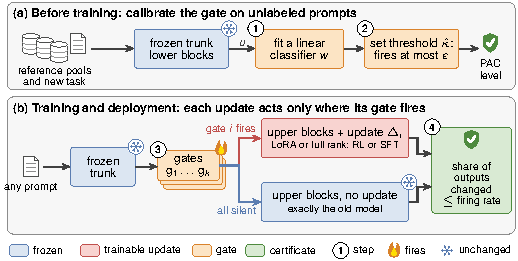
\includegraphics[width=\linewidth]{figures/firegate_overview.pdf}
\caption{Overview of \method{}. (a) Before training, the gate's classifier is fitted (1) and calibrated on unlabeled
prompts (2), which fixes its firing rate. (b) Each task's update acts only where its gate fires (3); elsewhere the model is
exactly the old one, so at most that share of outputs changes (4). The update can be a LoRA or a full-rank change of
the upper blocks, trained by RL or SFT, or a separately trained model behind a prompt-time gate.}
\label{fig:arch}
\end{figure}

\begin{theorem}[Coupling certificate]
\label{thm:coupling}
For every prompt distribution $D$, every decoding rule, and every update $\Delta$,
\begin{equation*}
\TV\big(P^D_{\pi_{\Delta,g}},P^D_{\pold}\big)\;\le\;\varphi_g(D):=P^D_{\pold}\big(\Fire_g\big).
\end{equation*}
Moreover $P^D_{\pi_{\Delta,g}}(\Fire_g)=\varphi_g(D)$, and with shared decoding randomness the response of
$\pi_{\Delta,g}$ equals that of $\pold$ on every run on which the gate does not fire.
\end{theorem}

\emph{Proof idea:} Run both models with the same uniform variables. By induction over positions and blocks, the runs
share every hidden state until the gate first fires, and the firing decision depends only on that shared prefix;
outside $\Fire_g$ the runs are identical, and the coupling inequality \citep{lindvall1992coupling} gives the bound.
All proofs are in \cref{app:proofs}. The bound is on the average over $D$: it says nothing about any single prompt, about prompts outside $D$, or about how responses change where the gate fires (\cref{tab:status}).

The certificate does not depend on $\Delta$, and no bound that depends only on the gate and holds for every
update can improve it by more than a factor $1-\eta$:

\begin{proposition}[Tightness]
\label{prop:tight}
Suppose an update can place all probability on a token $a^\dagger$ at the positions where it is active, and
$\pold$ gives $a^\dagger$ probability at most $\eta$ at those positions. Then
$\TV(P^D_{\pi_{\Delta,g}},P^D_{\pold})\ge(1-\eta)\,\varphi_g(D)$.
\end{proposition}

Without a gate ($g\equiv1$) some update drifts by nearly one (\cref{prop:tight,rem:nogate}).

\textbf{A certified switch for any trained model:} A prompt-time gate decides once: its decision
$G(x)=g(u_{|x|}(x))$ depends on $x$ alone, as the trunk is frozen and attention causal.

\begin{corollary}[Certified switch]
\label{cor:switch}
Let $G$ be the decision of a prompt-time gate and $\pi'$ any policy. The switch $\pi_{\pi',G}$ answers $x$ with
$\pi'$ if $G(x)=1$ and with $\pold$ otherwise. \Cref{thm:coupling} holds for $\pi_{\pi',G}$ with
$\varphi_g(D)=D(G=1)$, and its response equals $\pold$'s wherever $G(x)=0$.
\end{corollary}

The certificate thus takes two forms. Trained under its gate, an update acts only where the gate fires, as in
parameter isolation \citep{aljundi2017expertgate,liang2025gainlora} but with no task label at inference; behind a
switch, any trained model is certified but keeps its own forgetting (\cref{sec:res-calib}).

\subsection{Calibration without behaviour labels}

The certificate is a firing probability of the old model, so it can be estimated, and the threshold set, before
training, from unlabeled prompts and the old model's responses.

\begin{proposition}[Estimation on any distribution]
\label{prop:cp}
Roll out $\pold$ on $n$ i.i.d.\ prompts from $D$, independent of $g$, and let $X$ be the number of firings. With probability at least
$1-\delta$, $\varphi_g(D)\le\mathrm{CP}_{\delta}(X,n)$, the one-sided Clopper--Pearson bound \citep{clopper1934}.
\end{proposition}

A scored gate $g_\kappa(u)=\ind[w(u)>\kappa]$ fires on $s$ only if $S(s)=\max_{t}w(u_t(s))>\kappa$, the maximum
running over the positions where it is evaluated, so $\varphi_{g_\kappa}(D)\le P^D_{\pold}(S>\kappa)$. The threshold $\kappa$ is set
before training with the Neyman--Pearson umbrella algorithm \citep{tong2018np}, a training-conditional conformal bound
\citep{vovk2012conditional,bates2021rcps}, applied to each reference component with a union bound, which gives a
probably approximately correct (PAC) guarantee.

\begin{theorem}[PAC calibration]
\label{thm:calib}
Let $w$ and $\pold$ be fixed independently of the calibration set. For each reference component $c=1,\dots,C$,
draw $n_c$ i.i.d.\ calibration trajectories of $\pold$ on $D_c$ and let $S^c_{(1)}\le\dots\le S^c_{(n_c)}$ be their sorted
scores. Let $k_c=\min\{k:\Pr[\mathrm{Bin}(n_c,1-\varepsilon)\ge k]\le\delta/C\}$, $\hat\kappa_c=S^c_{(k_c)}$
($+\infty$ if $k_c>n_c$), and $\hat\kappa=\max_c\hat\kappa_c$. Then with probability at least $1-\delta$ over the
calibration draws, $\varphi_{g_{\hat\kappa}}(D_c)\le\varepsilon$ for every $c$.
\end{theorem}

\textbf{Certified level and its check:} On each reference component the certificate is the level $\varepsilon$, fixed
before training with confidence $1-\delta$ over the calibration draw, for prompts drawn like the calibration prompts.
The level attained is lower, on average at most 1.7\% for the 700 Dolly calibration prompts used here (\cref{prop:size}).
It carries over to mixtures of components, and becomes $\varepsilon+\theta$ or $M\varepsilon$ within TV distance $\theta$
of a component or at density ratio at most $M$ to it (\cref{prop:transfer}). Held-out prompts of a component check
the level with a one-sided binomial test. A prompt-time gate's firing depends on the prompt alone, so its certificate
holds under every decoding rule; an anytime gate's holds for the rule it was calibrated under. On a distribution far from every component, such as MMLU, the only certificate is the
bound of \cref{prop:cp} from a sample of it, which holds for that distribution only and can be large (\cref{tab:certs}).

\subsection{Streams and prompts unlike the task}

In a stream, stage $k$ adds a gate $g_k$ on the same frozen trunk and a LoRA $\Delta_k$ gated by its own
latch, and leaves $\Delta_1,\dots,\Delta_{k-1}$ and $g_1,\dots,g_{k-1}$ unchanged.

\begin{theorem}[Stream certificate]
\label{thm:stream}
For every $j<k$ and every distribution $D$,
$\TV\big(P^D_{\pi_k},P^D_{\pi_j}\big)\le P^D_{\pi_j}\big(\bigcup_{i=j+1}^{k}\Fire_{g_i}\big)
\le\sum_{i=j+1}^{k}P^D_{\pi_j}\big(\Fire_{g_i}\big)$.
\end{theorem}

Drift on task $j$ is bounded by the firing of the later gates on $\pi_j$'s own trajectories, so earlier tasks
are protected without replaying their labels, and calibrating each stage at $\varepsilon$ certifies the union of $K$
stages at $K\varepsilon$ with confidence $1-K\delta$ (\cref{cor:compose}). A prompt-time union can also be certified directly
as one gate, by \cref{prop:cp} on fresh prompts that no stage used, at confidence $1-\delta$ and at a level that does
not grow with $K$. Anytime gates need fresh calibration
prompts at each stage (\cref{cor:compose}); the gates here reuse them, so their later stages are only checked held out.

A classifier trained to tell the new task from the reference extrapolates on prompts unlike both, and may fire there. A
second test, whether the prompt lies in the new task's region, bounds the firing on such prompts.

\begin{proposition}[Two-sided gate]
\label{prop:twosided}
Let $g_\kappa=\ind[w>\kappa]$ be a prompt-time gate with score $w(u_{|x|}(x))$, $R$ a set of prompts, both fixed
independently of the calibration prompts, and $h_\kappa=g_\kappa\ind_R$. (a) For every $\kappa$ and every $D$,
$\varphi_{h_\kappa}(D)\le\min\{\varphi_{g_\kappa}(D),\,D(R)\}$. (b) \Cref{thm:calib} applied to the score equal
to $w$ on $R$ and to $-\infty$ off $R$ calibrates $h$ with the same guarantee on every reference component. (c) Let
$R=\{x:d(x)\le\hat\tau\}$ for a function $d$ fixed independently of $n$ i.i.d.\ prompts of $\Dnew$, and $\hat\tau$ the
$k$-th smallest value of $d$ on them, or $+\infty$ if $k>n$. If $\Pr[\mathrm{Bin}(n,1-\alpha)\ge k]\le\delta$,
then $\Dnew(R^c)\le\alpha$ with probability at least $1-\delta$; if $k\ge\lceil(n+1)(1-\alpha)\rceil$, then
$\E\big[\Dnew(R^c)\big]\le\alpha$.
\end{proposition}

The region is not a safety filter: it excludes prompts unlike the task, not prompts written like it, such as
harmful requests in the task's format, which must be added to the reference. With 1{,}000 unlabeled RL prompts
and $\alpha=0.02$, it misses at most 2.9\% of new-task prompts with probability 0.95.

\textbf{Checks without labels:}\label{sec:monitor} An audit evaluates only fired prompts (\cref{prop:decomp}), an anytime-valid test
\citep{ramdas2023gametheoretic} on the firing indicator raises an alarm when traffic fires more often than certified
(\cref{prop:monitor}), and raising a threshold repairs a failed certificate without retraining (\cref{prop:repair}).

% =====================================================================================
\section{The price of certification}
\label{sec:limit}

An update that changes at most a share $\varepsilon$ of behaviour on the reference can change the new task only
as far as a test of level $\varepsilon$ tells the two apart, gated or not.

\begin{theorem}[Certified plasticity limit]
\label{thm:limit}
Let $\pnew$ be any policy, gated or not, and $\rho(x)=\TV(\pnew(\cdot\mid x),\pold(\cdot\mid x))$. If
$\E_{\Dref}\rho\le\varepsilon$, then $\E_{\Dnew}\rho\le\beta^\ast(\varepsilon)$, the power of the
size-$\varepsilon$ Neyman--Pearson test of $\Dref$ against $\Dnew$, and, for $\varepsilon\in(0,1)$,
\begin{equation}
\beta^\ast(\varepsilon)\le\frac{\KL(\Dnew\|\Dref)+\log 2}{\log(1/\varepsilon)}.
\label{eq:limit}
\end{equation}
The expected reward gain on $\Dnew$ is at most $\E_{\Dnew}\rho$ times the reward range. If the update can move
the response distribution of every prompt where it acts as \cref{prop:tight} assumes, and the likelihood ratio of
$\Dnew$ to $\Dref$ is a function of the trunk feature $u_{|x|}(x)$, then $\beta^\ast(\varepsilon)$ is attained up to
the factor $1-\eta$ by a gated update whose prompt-time gate is the likelihood-ratio test, randomised on ties
(deterministic if the ratio has no atoms).
\end{theorem}

\begin{figure}[t]
\centering
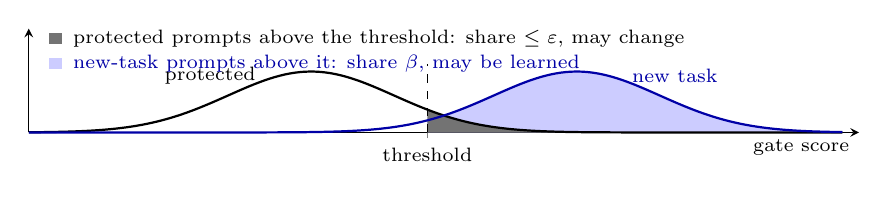
\begin{tikzpicture}
\begin{axis}[width=\linewidth, height=2.9cm, axis lines=left, xmin=-3.4, xmax=6.6, ymin=0, ymax=0.68,
  ytick=\empty, xtick={1.4}, xticklabels={threshold}, tick label style={font=\scriptsize},
  xlabel={gate score}, label style={font=\scriptsize}, xlabel style={at={(1,0)}, anchor=north east, yshift=1pt},
  samples=160, clip=false]
\addplot[draw=none, fill=blue!20, domain=1.4:6.4] {exp(-(x-3.2)^2/2)/sqrt(2*pi)} \closedcycle;
\addplot[draw=none, fill=black!55, domain=1.4:6.4] {exp(-x^2/2)/sqrt(2*pi)} \closedcycle;
\addplot[black, thick, domain=-3.4:6.4] {exp(-x^2/2)/sqrt(2*pi)};
\addplot[blue!65!black, thick, domain=-3.4:6.4] {exp(-(x-3.2)^2/2)/sqrt(2*pi)};
\draw[dashed] (axis cs:1.4,0) -- (axis cs:1.4,0.45);
\node[font=\scriptsize, anchor=east] at (axis cs:-0.55,0.37) {protected};
\node[font=\scriptsize, anchor=west, text=blue!65!black] at (axis cs:3.75,0.37) {new task};
\node[font=\scriptsize, anchor=north west, align=left, inner sep=1pt] at (axis cs:-3.2,0.69)
  {\textcolor{black!55}{\rule{1.6ex}{1.3ex}}\, protected prompts above the threshold: share $\le\varepsilon$, may change\\[1pt]
   \textcolor{blue!20}{\rule{1.6ex}{1.3ex}}\, \textcolor{blue!65!black}{new-task prompts above it: share $\beta$, may be learned}};
\end{axis}
\end{tikzpicture}
\caption{The certificate and its price, schematically. At most a share $\varepsilon$ of protected prompts lie above the
threshold, the only ones whose outputs can change; the update acts only on the share $\beta$ of new-task prompts above
it.}
\label{fig:np}
\end{figure}

In words, an update can change the new task only as far as a test can tell its prompts from the reference, whether
it is gated, regularised, replays data or uses orthogonal or null-space LoRA (\cref{fig:np}). The first claim is the Neyman--Pearson lemma \citep{neyman1933}; the KL form is rarely informative
for distinct tasks (\cref{rem:klvacuous}). With a level per component, as \cref{thm:calib} sets them, the limit is that of the
generalised Neyman--Pearson lemma \citep{dantzig1951fundamental,lehmann2022testing}: a likelihood-ratio test against a
weighted sum of components, whose weights price each component's level (\cref{prop:percomp}). Where the limit is
known (\cref{app:npgap}), the linear score comes within about a point of it under a shift with enough prompts, PAC
calibration costs about 5 points, near the 4 that \cref{prop:size} predicts, and under a change of spread only a quadratic
score comes close. On real tasks the limit is unknown, and the coverage of any gate is a lower bound on
$\beta^\ast(\varepsilon)$, not an estimate of it. Responses add no evidence about a prompt's source
(\cref{prop:noevidence}), so an optimal gate needs only the prompt, as \methodp{} reads, and thresholding an estimated
density ratio loses at most its $L^1$ error in coverage, while calibration keeps the certificate valid
(\cref{prop:estimated}).

\begin{corollary}[A certificate before training confines every large change]
\label{cor:gate}
Let $\mathcal U$ be the set of models that training can reach, and $A$ a set of prompts on which one $\pi\in\mathcal U$
moves every response distribution by at least $1-\eta$ in TV, as an unconstrained update can on every prompt
(\cref{prop:tight}). If every $\pi\in\mathcal U$ changes at most a share $\varepsilon$ of outputs on $\Dref$, then
$\Dref(A)\le\varepsilon/(1-\eta)$ and $\Dnew(A)\le\beta^\ast\big(\varepsilon/(1-\eta)\big)$.
\end{corollary}

So under a certificate before training each reachable model changes outputs strongly only on prompts of reference
mass about $\varepsilon$. Different models may use different regions, so this does not force one common gate; a gate
is the simplest way to fix the region in advance, and a likelihood-ratio gate on the trunk can attain the limit; a penalty bounds only the weights that
optimise it, and only their sampled outputs (\cref{rem:nogate}). A class that moves no response by more than $\varepsilon$ is
certified at $\varepsilon$ without a gate, but changes new-task responses by at most $\varepsilon$ too.

\begin{proposition}[Gain behind a gate]
\label{prop:switchgain}
Let $G$ be the decision of a prompt-time gate, $\pi'$ any policy, $\Delta r(x)$ the difference between the expected rewards of $\pi'$
and $\pold$ on prompt $x$, $\bar G=\E_{\Dnew}\Delta r$ the gain of $\pi'$ itself, $\beta=\Dnew(G=1)\in(0,1)$, and $\bar
G_1,\bar G_0$ the means of $\Delta r$ on new-task prompts with $G=1$ and $G=0$. The gain of the switch $\pi_{\pi',G}$
on $\Dnew$ is $\beta\bar G_1=\beta\bar G+\beta(1-\beta)(\bar G_1-\bar G_0)$.
\end{proposition}

The coverage $\beta$ is the gate's firing rate on unlabeled new-task prompts, so it is estimated before training;
the gain kept is $\beta\bar G$ plus a covariance term that the certificate does not control. The term vanishes as
$\beta\to1$ and when the prompts the gate misses would gain as much as the others, so $\beta\bar G$ is a prediction, tested in \cref{sec:res-switch}, not a bound.

% =====================================================================================
\section{\method{} in practice}
\label{sec:method}

The gate is a linear classifier with score $w_k(u)=a_k^\top\big((\bar u-\mu)/\sigma\big)+b_k$, where
$\bar u=u/\mathrm{rms}(u)$ and $\mu,\sigma$ are per-coordinate statistics. Class-balanced logistic regression fits it
to separate prompts of the new task from those of the reference components; its only supervision is which pool a
prompt came from. Fitting and calibration use disjoint prompts, as \cref{thm:calib} requires. \methodp{} scores the
last prompt token; \methoda{} scores every position after the template prefix; a whole-sequence variant of \methodp{}
applies the LoRA to the whole sequence once the gate has fired, as a switch does. A LoRA is trained under its own
gate, where rollouts on which the gate does not fire carry no gradient, or by any method and placed behind the gate
afterwards (\cref{cor:switch}). The two-sided region keeps prompts whose Mahalanobis distance to the new task's
fitting prompts, in the classifier's feature space, is below its $1-\alpha$ quantile on unlabeled RL prompts, with
$\alpha=0.02$ (\cref{alg:tripwire}, \cref{app:impl}).

\textbf{Choosing the reference:} The certificate covers the components one samples, so choosing them is part of the
method, and each choice can be priced before training. (1) Calibrate on every kind of prompt whose behaviour must not
change; a sample of the deployment's own unlabeled traffic can itself be a component. (2) Check any other unlabeled
pool before training, from one trunk pass: the bound of \cref{prop:cp} on a sample of it is its certificate. (3) Use
the two-sided gate, which caps the firing on any pool at its mass in the task's region and misses about a share
$\alpha$ of the task's prompts. (4) If a pool still fires more often than $\varepsilon$, such as harmful requests written in the task's
format, add it as a component, the \emph{remedy}. (5) If the task cannot be told apart from some component, such as
general chat, calibrate only on the components to \emph{protect}: they are then certified for any model, and the
gate's firing on the others, estimated before training, says how much of them may change. The coverage $\beta$ after
each step is the price of that step, by \cref{prop:switchgain}, and the weights of \cref{prop:percomp} say which
component sets it. Steps (1) and (2) with \cref{thm:calib} give the certificate; steps (3)--(5) change only which
prompts it covers and the coverage. A distribution at density ratio at most $M$ to a component is certified at
$M\varepsilon$ (\cref{prop:transfer}).

\textbf{Deciding before training:} The coverage $\beta$ is measured on unlabeled task prompts before any training, and
a model behind the gate keeps about $\beta\bar G$ of its gain (\cref{prop:switchgain}). The recipe therefore also says
whether certification is worth its price. With $\beta$ near 1, as on the task streams, almost all of the gain is kept;
with $\beta$ near 0, as on Concise (0.7\%), the components to protect must be narrowed or the task left ungated.
Certification is cheapest for tasks whose prompts are easy to tell apart from what must stay, and most costly for
chat-like tasks, as \cref{thm:limit} predicts.

% =====================================================================================
\section{Experiments}
\label{sec:experiments}

\subsection{Setup}
\label{sec:setup-main}

\textbf{Models and tasks:} Qwen2.5-1.5B- and 7B-Instruct \citep{qwen2025qwen25}, OLMo-2-7B-Instruct
\citep{olmo2024olmo2}, Llama-3.2-3B- and 3.1-8B-Instruct \citep{grattafiori2024llama3}, DeepSeek-LLM-7B-Chat
\citep{bi2024deepseekllm} and Mistral-7B-Instruct \citep{jiang2023mistral}. Two streams of tasks that are easy to tell
apart from the reference: GSM8K \citep{cobbe2021gsm8k}, Countdown \citep{pan2025tinyzero} and Knights and Knaves
\citep{xie2024kk,xie2025logicrl}, and a five-task stream that adds MATH \citep{hendrycks2021math} and Sudoku. An
\emph{overlap ladder} of tasks whose prompts resemble the reference more and more: IF, Dolly requests with a
format constraint \citep{zhou2023ifeval}; NQ, closed-book Natural Questions
\citep{kwiatkowski2019nq,lee2019latent}; and Concise-ctx and Concise, Dolly requests with or without a
passage, rewarded for a short answer. A natural task that overlaps chat: SQuAD~2.0 \citep{rajpurkar2018squad2},
rewarded for the gold answer or for abstaining. The gate reads block 9 of 28 in Qwen2.5 (about 0.3 of the
depth in every model); LoRA of rank 16 above it; GRPO for 150 steps per task, 16 prompts $\times$ 8 samples; three
seeds; fitting/calibration: Dolly 600/700, AdvBench 100/170, task-like 900/700 (\cref{app:full}).

\textbf{Methods:} \methodp{}, its whole-sequence variant and \methoda{} at $\varepsilon=0.03$, against eleven baselines
with the same LoRA and budget: Seq-GRPO, an ungated LoRA per task; +KL to the previous model
\citep{shenfeld2026razor}; +Ref-KL, the same penalty on the reference prompts the gate uses \citep{li2018lwf};
null-space LoRA \citep{liang2024inflora}, EWC \citep{kirkpatrick2017ewc} and A-GEM \citep{chaudhry2019agem} on the same
prompts; LoRA scaling \citep{wortsman2022robust}, O-LoRA \citep{wang2023olora}, replay, safety replay
\citep{pham2025preventing}, and an uncalibrated router. The \emph{deployed} gate is \methodp{}'s classifier at
$\varepsilon=0.03$; as \cref{cor:switch} allows, every ungated run is also evaluated behind it. Two gates appear in
the main text. The deployed gate, steps (1) and (2) of \cref{sec:method}, gives the coverage, gain and switch results
unless a result is marked otherwise (\cref{tab:variants}). The chosen gate of each experiment is what the full recipe selects: two-sided,
with the remedy or a protected set where steps (4) and (5) apply. It was fixed before the external tests of
\cref{sec:res-gates}.

\textbf{Reference pools and evaluation:} Gates are calibrated with $\delta=0.05$ on unlabeled prompts of four kinds:
Dolly-15k requests \citep{conover2023dolly}, AdvBench harmful requests \citep{zou2023gcg}, task-like prompts (ARC,
CommonsenseQA, OpenBookQA, BoolQ, Alpaca, MBPP) and stored prompts of earlier tasks. The share of changed
responses is measured on held-out Dolly and AdvBench prompts and on XSTest \citep{rottger2024xstest} and MMLU
\citep{hendrycks2021mmlu}, which are never calibrated on. \Cref{app:full} gives every setting;
\cref{tab:protocol} marks what was fixed before its evidence.

\begin{table}[t]
\centering
\footnotesize
\setlength{\tabcolsep}{2.2pt}
\caption{Certified levels and their checks (\%). Every reference component, Dolly among them, is certified at 3\% with
probability 0.95 (\cref{thm:calib}). Dolly, MMLU: firing on held-out prompts and, in
brackets, its 95\% Clopper--Pearson bound (\cref{prop:cp}), a check on Dolly and the only certificate on MMLU. $\beta$:
firing on the unlabeled RL prompts, which also set the two-sided gate's region, so $\beta\le98$ there. Streams: union
of per-stage gates, each at 3\%. 10k: the bound from 10{,}000 fresh Dolly requests (\cref{tab:ledger}).}
\label{tab:certs}
\resizebox{\ifdim\width>\linewidth\linewidth\else\width\fi}{!}{%
\begin{tabular}{l rrrr rrr}
\toprule
 & \multicolumn{4}{c}{deployed gate} & \multicolumn{3}{c}{two-sided gate} \\
\cmidrule(lr){2-5}\cmidrule(lr){6-8}
Experiment & $\beta\uparrow$ & Dolly$\downarrow$ & 10k$\downarrow$ & MMLU$\downarrow$ & $\beta\uparrow$ & Dolly$\downarrow$ & MMLU$\downarrow$ \\
\midrule
NQ, Qwen 1.5B & \ovgNqRatioAPower & \ovgNqRatioADolly{} [\ovgNqRatioACpDolly] & 1.7 & \ovgNqRatioAMmlu{} [\ovgNqRatioACpMmlu] & \ovgNqTwoAPower & \ovgNqTwoADolly{} [\ovgNqTwoACpDolly] & \ovgNqTwoAMmlu{} [\ovgNqTwoACpMmlu] \\
NQ, Qwen 7B & \ovgNqsevenRatioAPower & \ovgNqsevenRatioADolly{} [\ovgNqsevenRatioACpDolly] & 2.5 & \ovgNqsevenRatioAMmlu{} [\ovgNqsevenRatioACpMmlu] & \ovgNqsevenTwoAPower & \ovgNqsevenTwoADolly{} [\ovgNqsevenTwoACpDolly] & \ovgNqsevenTwoAMmlu{} [\ovgNqsevenTwoACpMmlu] \\
NQ, OLMo-2 7B & \ovgNqolmoRatioAPower & \ovgNqolmoRatioADolly{} [\ovgNqolmoRatioACpDolly] & 2.2 & \ovgNqolmoRatioAMmlu{} [\ovgNqolmoRatioACpMmlu] & \ovgNqolmoTwoAPower & \ovgNqolmoTwoADolly{} [\ovgNqolmoTwoACpDolly] & \ovgNqolmoTwoAMmlu{} [\ovgNqolmoTwoACpMmlu] \\
IF, Qwen 1.5B & \ovgIfcRatioAPower & \ovgIfcRatioADolly{} [\ovgIfcRatioACpDolly] & -- & \ovgIfcRatioAMmlu{} [\ovgIfcRatioACpMmlu] & \ovgIfcTwoAPower & \ovgIfcTwoADolly{} [\ovgIfcTwoACpDolly] & \ovgIfcTwoAMmlu{} [\ovgIfcTwoACpMmlu] \\
IF, Qwen 7B & \ovgIfcsevenRatioAPower & \ovgIfcsevenRatioADolly{} [\ovgIfcsevenRatioACpDolly] & -- & \ovgIfcsevenRatioAMmlu{} [\ovgIfcsevenRatioACpMmlu] & \ovgIfcsevenTwoAPower & \ovgIfcsevenTwoADolly{} [\ovgIfcsevenTwoACpDolly] & \ovgIfcsevenTwoAMmlu{} [\ovgIfcsevenTwoACpMmlu] \\
Concise-ctx, 1.5B & \ovgConcisectxRatioAPower & \ovgConcisectxRatioADolly{} [\ovgConcisectxRatioACpDolly] & -- & \ovgConcisectxRatioAMmlu{} [\ovgConcisectxRatioACpMmlu] & \ovgConcisectxTwoAPower & \ovgConcisectxTwoADolly{} [\ovgConcisectxTwoACpDolly] & \ovgConcisectxTwoAMmlu{} [\ovgConcisectxTwoACpMmlu] \\
3 tasks, Qwen 1.5B & \ovgStreamRatioAPower & \ovgStreamRatioADolly{} [\ovgStreamRatioACpDolly] & 3.3 & \ovgStreamRatioAMmlu{} [\ovgStreamRatioACpMmlu] & \ovgStreamTwoAPower & \ovgStreamTwoADolly{} [\ovgStreamTwoACpDolly] & \ovgStreamTwoAMmlu{} [\ovgStreamTwoACpMmlu] \\
3 tasks, Qwen 7B & \ovgStreamsevenRatioAPower & \ovgStreamsevenRatioADolly{} [\ovgStreamsevenRatioACpDolly] & 2.8 & \ovgStreamsevenRatioAMmlu{} [\ovgStreamsevenRatioACpMmlu] & \ovgStreamsevenTwoAPower & \ovgStreamsevenTwoADolly{} [\ovgStreamsevenTwoACpDolly] & \ovgStreamsevenTwoAMmlu{} [\ovgStreamsevenTwoACpMmlu] \\
5 tasks, Qwen 1.5B & \ovgStreamfiveRatioAPower & \ovgStreamfiveRatioADolly{} [\ovgStreamfiveRatioACpDolly] & 4.5 & \ovgStreamfiveRatioAMmlu{} [\ovgStreamfiveRatioACpMmlu] & \ovgStreamfiveTwoAPower & \ovgStreamfiveTwoADolly{} [\ovgStreamfiveTwoACpDolly] & \ovgStreamfiveTwoAMmlu{} [\ovgStreamfiveTwoACpMmlu] \\
\bottomrule
\end{tabular}}
\end{table}

% -------------------------------------------------------------------------------------
\subsection{The certificate holds as stated}
\label{sec:res-cert}

\newcommand{\thou}[1]{\pgfmathprintnumber[int detect, 1000 sep={,}, assume math mode=true]{#1}}%
\textbf{Exactness:} No response on which the gate was silent ever changed, under greedy decoding or under sampling
(\cref{tab:decode}): the implementation realises \cref{thm:coupling} exactly.

\textbf{The calibrated level:} Held-out prompts are consistent with the level of 3\% (\cref{tab:certs}), which 400 cannot
confirm: the single-task deployed gates fire on at most 3.2\% of held-out Dolly prompts (bounds up to 5.1\%) and on no
held-out harmful request. On 10{,}000 fresh Dolly requests they fire on 1.5--2.2\% (bounds at most 2.5\%,
\cref{tab:ledger}), as \cref{prop:size} predicts, and the stream unions' bounds of 2.8--4.5\% certify each union far
below $K\varepsilon$ (\cref{prop:cp}).

% -------------------------------------------------------------------------------------
\subsection{Certified updates kept about the share $\beta$ of the gain}
\label{sec:res-switch}\label{sec:res-drift}\label{sec:res-scale}

\textbf{Ungated updates change most reference responses:} Seq-GRPO changes over 90\% of Dolly responses on every
task, none of which it was trained on, and the regularisers change most of them too, including those built from the
gate's own reference prompts (\cref{tab:main}); on NQ it also lowers refusal, though its data concern no refusals (\cref{tab:overlap_nq}; \citealp{qi2024finetuning}). On NQ and SQuAD~2.0, every ungated setting (26 on NQ) changes at
least 51\% of Dolly responses, even at LoRA scale 0.02 or KL weight 100, since a penalty limits sampled outputs and a
small change still flips greedy ones (\cref{rem:nogate}); gates that certify Dolly change 0.5--3.5\%
(\cref{fig:frontier,tab:matched}). A changed response may be a
rewording, but the drift is real: response lengths alone bound Seq-GRPO's TV distance on NQ far above the certified level (\cref{tab:decode}).
Average scores can stay flat while responses change: on the three-task stream Seq-GRPO moves AdvBench refusal and
MMLU accuracy by at most a point but lowers XSTest over-refusal by 15.5 points (\cref{tab:main}). The certificate
bounds every such score at once, including those nobody measured.

\newcommand{\NSdir}{\resdir/v2_overlap_q15/switch}
\begin{figure*}[t]
\centering
\IfFileExists{\Odir/overlap_frontier_tw.dat}{%
\begin{tikzpicture}
\begin{groupplot}[group style={group size=2 by 1, horizontal sep=0.35cm, y descriptions at=edge left},
  height=4.6cm, ymin=-0.6, ymax=7.6, ytick={0,2,4,6},
  tick label style={font=\footnotesize}, label style={font=\footnotesize}, title style={font=\footnotesize\bfseries, yshift=-0.6ex},
  every axis plot/.append style={line width=0.9pt}, grid=major, grid style={black!8}]
\nextgroupplot[width=0.56\textwidth, xmin=-1.5, xmax=31, xtick={0,10,20,30}, ylabel={NQ gain (points)},
  title={gated}]
\addplot[orange!85!black, mark=*, mark size=1.5pt] table[x=chg, y=gain] {\Odir/overlap_frontier_tw.dat};
\addplot[red!75!black, mark=diamond*, mark size=2pt] table[x=chg, y=gain] {\Odir/overlap_frontier_twp.dat};
\addplot[black, mark=star, mark size=2.2pt] table[x=chg, y=gain] {\NSdir/switch_frontier_seq.dat};
\addplot[only marks, black, mark=x, mark size=2.6pt, restrict x to domain=-5:40] table[x=chg, y=gain] {\Odir/overlap_frontier_base.dat};
\addplot[only marks, black, mark=asterisk, mark size=2.6pt] table[x=chg, y=gain] {\Odir/overlap_frontier_oracle.dat};
\node[font=\scriptsize, text=orange!85!black, anchor=north] at (axis cs:20,2.05) {\methoda{}};
\node[font=\scriptsize, text=red!75!black, anchor=south] at (axis cs:22,6.0) {\methodp{}};
\node[font=\scriptsize, anchor=north, align=center, inner sep=1pt] at (axis cs:20,4.95) {Seq-GRPO behind\\[-1pt]the gate};
\node[font=\scriptsize, anchor=south] at (axis cs:6.75,5.75) {router};
\node[font=\scriptsize, anchor=south] at (axis cs:1.4,5.6) {oracle};
\nextgroupplot[width=0.47\textwidth, xmin=52, xmax=101, xtick={60,80,100}, title={ungated},
  legend to name=frontierleg, legend columns=6, legend style={font=\footnotesize, draw=none, column sep=6pt},
  legend cell align=left]
\addplot[blue!60!black, dashed, mark=square*, mark size=1.4pt] table[x=chg, y=gain] {\Odir/overlap_frontier_kl.dat};
\addlegendentry{+KL}
\addplot[teal!70!black, dashed, mark=triangle*, mark size=1.8pt] table[x=chg, y=gain] {\Odir/overlap_frontier_refkl.dat};
\addlegendentry{+Ref-KL}
\addplot[violet!70!black, dashed, mark=pentagon*, mark size=1.8pt] table[x=chg, y=gain] {\Odir/overlap_frontier_null.dat};
\addlegendentry{null-space LoRA}
\addplot[brown!70!black, dashed, mark=star, mark size=1.8pt] table[x=chg, y=gain] {\Odir/overlap_frontier_ewc.dat};
\addlegendentry{+EWC}
\addplot[gray!80!black, dashed, mark=o, mark size=1.5pt, restrict x to domain=1:101] table[x=chg, y=gain] {\Odir/overlap_frontier_scale.dat};
\addlegendentry{LoRA scale}
\addplot[only marks, black, mark=+, mark size=2.6pt, restrict x to domain=50:101] table[x=chg, y=gain] {\Odir/overlap_frontier_base.dat};
\addlegendentry{Seq-GRPO, A-GEM}
\end{groupplot}
\node[font=\footnotesize, anchor=north] at ($(group c1r1.south east)!0.5!(group c2r1.south west) + (0,-0.5)$) {Dolly responses changed (\%)};
\end{tikzpicture}\par\vspace{-1pt}\ref*{frontierleg}
}{\placeholder{Trade-off figure.}}
\caption{NQ, Qwen2.5-1.5B: gain against Dolly responses changed, mean of three seeds. Each curve sweeps one knob:
the level $\varepsilon$ for the gates and Seq-GRPO behind \methodp{}'s gate, the coefficient, energy share, weight or
scale for the ungated methods. The router uses its logit-0 rule; the oracle knows each prompt's task
(\cref{tab:overlap_nq}).}
\label{fig:frontier}
\end{figure*}

\textbf{The gain kept follows the coverage:} \Cref{tab:fam} places Seq-GRPO behind the deployed gate of seven models.
On IF the gate fires on nearly every new-task prompt and the switch keeps all of the gain; on NQ, where the tasks
overlap, it keeps within one point of $\beta\bar G$ on every model. On TriviaQA, a task first used after every setting was fixed, all seven predictions written before its data were downloaded hold (\cref{app:trivia}): behind the gate Seq-GRPO keeps 23.1 of its 24.6-point gain, against 22.3 predicted before training, and changes 3.5\% of Dolly responses instead of 95.8\%. Given the trained model's gain $\bar G$, the deployed IF gates have $\beta=1$, where the prediction is exact by
construction; where $\beta<1$ it is off by 0.5 points on average
(\cref{fig:switchpred}), and by 0.3--0.4 on NQ as the threshold sweeps $\beta$ from 0.1 to 0.9, though by up to 4.1
on IF once the sweep lowers its $\beta$ (\cref{sec:exp-switch}): the trunk features barely
predict which prompts will gain, so on NQ a gate fitted to miss those prompts keeps as much as a random one, and only an
oracle that knows each prompt's gain does worse (\cref{tab:covcons});
on SQuAD~2.0 it keeps 18.5 points against 20.8, as missed prompts gained about 40 points against 22
(\cref{prop:switchgain}). The streams, full-rank GRPO and SFT behave alike (\cref{tab:deploy,tab:pilot}).

\begin{figure*}[t]
\centering
\IfFileExists{\OVdir/switch_pred.dat}{%
\begin{tikzpicture}
\begin{groupplot}[group style={group size=2 by 1, horizontal sep=1.1cm},
  height=4.6cm, tick label style={font=\footnotesize}, label style={font=\footnotesize},
  title style={font=\footnotesize\bfseries, yshift=-0.6ex}, grid=major, grid style={black!8},
  scatter/classes={Nq={mark=*,red!70!black}, Nqseven={mark=*,red!70!black}, Nqolmo={mark=*,red!70!black},
    Ifc={mark=diamond,orange!85!black}, Ifcseven={mark=diamond,orange!85!black},
    Concisectx={mark=triangle*,violet!70!black}, Concise={mark=square*,gray!80!black}}]
\nextgroupplot[width=0.5\textwidth, xmin=-3, xmax=58, ymin=-3, ymax=58, xtick={0,20,40}, ytick={0,20,40},
  ylabel={measured gain (points)}, title={all experiments}, legend to name=predleg, legend columns=5,
  legend style={font=\footnotesize, draw=none, column sep=6pt}, legend cell align=left]
\addplot[gray, dashed, domain=-3:58, samples=2] {x};
\addlegendentry{$y=x$}
\addplot[scatter, only marks, mark size=2pt, scatter src=explicit symbolic, forget plot, fill opacity=0.7]
  table[x=pred, y=actual, meta=exp] {\OVdir/switch_pred.dat};
\addlegendimage{only marks, mark=*, red!70!black}\addlegendentry{NQ}
\addlegendimage{only marks, mark=diamond, orange!85!black}\addlegendentry{IF ($\beta=1$)}
\addlegendimage{only marks, mark=triangle*, violet!70!black}\addlegendentry{Concise-ctx}
\addlegendimage{only marks, mark=square*, gray!80!black}\addlegendentry{Concise}
\draw[black!50, thin] (axis cs:-1,-1) rectangle (axis cs:8,8);
\nextgroupplot[width=0.5\textwidth, xmin=-1, xmax=8, ymin=-1, ymax=8, xtick={0,2,4,6,8}, ytick={0,2,4,6,8},
  title={zoom: $0$--$8$ points}, ylabel={}]
\addplot[gray, dashed, domain=-1:8, samples=2] {x};
\addplot[scatter, only marks, mark size=2.2pt, scatter src=explicit symbolic, fill opacity=0.7]
  table[x=pred, y=actual, meta=exp] {\OVdir/switch_pred.dat};
\end{groupplot}
\node[font=\footnotesize, anchor=north] at ($(group c1r1.south east)!0.5!(group c2r1.south west) + (0,-0.5)$)
  {predicted gain behind the gate, $\beta\bar G$ (points)};
\end{tikzpicture}\par\vspace{-1pt}\ref*{predleg}
}{\placeholder{Predicted against measured gain behind the switch.}}
\caption{Gain kept behind the prompt-time gate against $\beta\bar G$ (\cref{prop:switchgain}; $\beta$ measured before
training, $\bar G$ the trained model's gain), every ungated method at three levels, mean over seeds; right: the box on
the left. On IF $\beta=1$; on the 78 other points the mean error is 0.3 points (0.5 where $\beta<1$), the largest 3.4.}
\label{fig:switchpred}
\end{figure*}

\begin{table}[t]
\centering
\footnotesize
\setlength{\tabcolsep}{2.5pt}
\caption{The switch on seven models from five families (three seeds, $\varepsilon=0.03$). $\bar G$, Chg.: Seq-GRPO's
gain (points) and changed Dolly responses (\%); $\beta$: firing on unlabeled RL prompts, before training; Kept: the
gain behind the deployed prompt-time gate; CP: 95\% Clopper--Pearson bound of its held-out Dolly firing (\%);
Non-fired: changed non-fired responses of the \methodp{} runs; $^\dagger$two of three runs.}
\label{tab:fam}
\resizebox{\ifdim\width>\linewidth\linewidth\else\width\fi}{!}{%
\begin{tabular}{l l rr r rrrr r}
\toprule
 & & \multicolumn{2}{c}{ungated} & & \multicolumn{4}{c}{behind the gate} & \\
\cmidrule(lr){3-4}\cmidrule(lr){6-9}
Model & Task & $\bar G$ & Chg. & $\beta$ & $\beta\bar G$ & Kept$\uparrow$ & Chg.$\downarrow$ & CP$\downarrow$ & Non-fired \\
\midrule
Qwen2.5-1.5B & IF & +38.7 & 93.3 & 100.0 & +38.7 & +38.7 & 1.5 & 2.9 & 0/4{,}797 \\
Qwen2.5-1.5B & NQ & +5.2 & 94.2 & 92.2 & +4.8 & +4.7 & 3.2 & 5.1 & 0/9{,}363 \\
Qwen2.5-7B & IF & +12.9 & 94.6 & 100.0 & +12.9 & +12.9 & 0.8 & 3.3 & 0/3{,}531 \\
Qwen2.5-7B & NQ & +3.8 & 94.6 & 97.9 & +3.7 & +3.8 & 2.8 & 4.5 & 0/9{,}310 \\
OLMo-2-7B & NQ & +5.9 & 91.2 & 96.8 & +5.7 & +5.7 & 2.2 & 3.9 & 0/9{,}303 \\
Llama-3.2-3B & IF & +14.3 & 94.1 & 100.0 & +14.3 & +14.3 & 1.7 & 3.3 & 0/3{,}783 \\
Llama-3.2-3B & NQ & +10.8 & 96.7 & 89.0 & +9.6 & +9.2 & 2.5 & 4.2 & 0/9{,}447 \\
Llama-3.1-8B & IF & +11.4 & 95.5 & 100.0 & +11.4 & +11.4 & 1.8 & 3.3 & 0/3{,}957 \\
Llama-3.1-8B & NQ & +7.1 & 99.9 & 95.5 & +6.7 & +6.8 & 2.5 & 4.2 & 0/9{,}342 \\
DeepSeek-LLM-7B & IF & +35.3 & 99.5 & 99.9 & +35.2 & +35.3 & 2.3 & 3.9 & 0/3{,}429 \\
DeepSeek-LLM-7B & NQ & +10.7 & 97.3 & 84.5 & +9.1 & +8.7 & 1.3 & 2.6 & 0/9{,}519 \\
Mistral-7B & IF & +34.8 & 98.5 & 100.0 & +34.8 & +34.8 & 1.0 & 2.3 & 0/4{,}008 \\
Mistral-7B & NQ & +9.5 & 98.8 & 93.0 & +8.8 & +7.9 & 2.3 & 3.9 & 0/6{,}270$^\dagger$ \\
\bottomrule
\end{tabular}}
\end{table}

% -------------------------------------------------------------------------------------
\subsection{Calibration, the switch and gated training}
\label{sec:res-calib}

\textbf{Calibration sets the level:} Five gates built from the same features and prompts, as a router or an expert
gate \citep{aljundi2017expertgate} would build them, fire on up to 31\% of Dolly prompts on NQ at their own
thresholds, which are set to separate the pools, not to keep the reference quiet; PAC-calibrated, they fire on at
most 3.2\% and still keep most of the gain (\cref{tab:zoo}). The score then sets only the coverage: four score
classes calibrated together, each at $\delta/4$, all keep protected harmful requests at most 1.6\% (\cref{tab:fixes}).
A Gaussian ratio covers 95.3\% of NQ, 85.4\% of SQuAD~2.0 and 56.7\% of Concise-ctx (protect + passages), the linear
classifier 90.2, 81.4 and 11.0\%, and the best score bounds $\beta^\ast$ from below; on 13 model--task pairs it covers at
most 7.0 points more (\cref{tab:scoregrid}), neither shown to reach the limit. Scores that see one pool cover
little, the one-class score no NQ prompt (\cref{fig:score}), a language model told the task 2.9\% (\cref{tab:llmgate}): a score needs both pools.



\begin{table}[t]
\centering
\scriptsize
\setlength{\tabcolsep}{1.6pt}
\caption{Five-task stream, Qwen2.5-1.5B, three seeds. Avg, BWT: mean accuracy over the five tasks after the stream
(base 29.9\%) and backward transfer; Dolly: held-out responses changed (\%), rewordings included (refusal,
over-refusal and MMLU changes on a stream: \cref{tab:main}); GB, time: peak memory and batched
generation time against the base model, gated LoRAs unmerged, one or all five firing (\cref{app:full-scale}). Each
stage is certified at 3\%, so the union at 15\% with probability at least 0.75 (\cref{cor:compose}); certified directly as
one gate on 10{,}000 fresh Dolly requests (\cref{prop:cp}), its Dolly firing is at most 4.5\% with probability 0.95
(\cref{tab:ledger}). One gate: the union of the five two-sided gates, set once to fire on at most 3\% of the shared
calibration prompts (\cref{prop:promptstream}); on 400 fresh Dolly prompts it fires on none, which certifies its Dolly
firing at 0.7\% with probability 0.95 (\cref{prop:cp}). --: not measured.}
\label{tab:deploy}
\begin{tabular}{l rr r r r}
\toprule
Deployment & Avg$\uparrow$ & BWT$\uparrow$ & Dolly$\downarrow$ & GB & Time \\
\midrule
Seq-GRPO, ungated & 46.5{\tiny$\pm$1.7} & $-$3.5{\tiny$\pm$0.7} & 91.8 & 8.1 & $\times$1.00 \\
\quad behind the gate & 46.5{\tiny$\pm$1.7} & $-$3.5{\tiny$\pm$0.7} & 4.8 & 10.9 & $\times$1.18 \\
\quad behind one gate & 46.3{\tiny$\pm$1.8} & -- & 0.0 & -- & -- \\
\methodp{}, gated training & 49.6{\tiny$\pm$2.9} & +0.0{\tiny$\pm$0.0} & 3.3 & 12.5 & $\times$1.25--2.59 \\
\bottomrule
\end{tabular}
\end{table}

\textbf{Training under the gate and the switch:} On single tasks neither gains consistently more
(\cref{tab:protect,tab:overlap_nq}); the switch certifies a model trained by any method at the cost of a second model
in memory (33.9 against 19.7\,GB at 7B). Gated training stores the same LoRAs as the ungated baselines; matched in memory and routing, its comparison is the router, which uses the same features and LoRAs without calibration: it changes no chat on the 3-task stream, but on NQ it fires on \ovlRouterFireDolly\% of Dolly prompts, a rate set by no level before training (\cref{tab:main,tab:overlap_nq}). On a stream, gated training keeps the earlier tasks, because their LoRAs and
gates are frozen and fire only on their own prompts, while the switch inherits the trained model's forgetting
(\cref{tab:deploy}); the higher average comes mostly from seeds in which Seq-GRPO loses Countdown or K\&K, and the time
grows with the number of unmerged LoRAs whose gates fire. One gate set for the whole stream at 3\%,
instead of 3\% per stage, is certified on fresh Dolly prompts at 0.7\% (\cref{prop:cp}) and keeps 46.3 of 46.5
points. On this evidence, three streams of three or five tasks on Qwen2.5 at 1.5B and 7B, the switch suits one task and gated training suits streams; longer streams are untested.

% -------------------------------------------------------------------------------------
\subsection{Protecting chosen behaviours}
\label{sec:res-protect}\label{sec:res-limit}

\begin{table*}[t]
\centering
\footnotesize
\setlength{\tabcolsep}{3.2pt}
\caption{Protecting chosen behaviours on SQuAD~2.0, a task that overlaps general chat (Qwen2.5-1.5B,
$\varepsilon=0.03$). Deployed: calibrated on every component; protect: on harmful and task-like prompts only;
+ passages: harmful requests followed by a passage added. $\beta$: coverage of RL prompts; changes in points;
responses changed (\%); harmful + passage: firing and refusal change on 250 such held-out requests, as given / as a
question (seed 0; else three seeds). Concise, Concise-ctx: \cref{tab:protect_concise,tab:remedy}.}
\label{tab:protect}
\begin{tabular}{l r r rr rrr rr}
\toprule
 & & & \multicolumn{2}{c}{Change} & \multicolumn{3}{c}{Responses changed (\%)} & \multicolumn{2}{c}{Harmful + passage} \\
\cmidrule(lr){4-5}\cmidrule(lr){6-8}\cmidrule(lr){9-10}
Method & $\beta\uparrow$ & Gain$\uparrow$ & Refusal & MMLU & AdvBench & MMLU & Dolly & Gate fires (\%) & Refusal \\
\midrule
\multicolumn{10}{l}{\emph{SQuAD~2.0: passage and question, rewarded for the gold answer or for abstaining}} \\
Seq-GRPO & -- & +24.4 & $-$0.3 & $-$2.9 & 77.1 & 49.3 & 99.3 & -- & $-$36.8 / $-$74.8 \\
\quad behind the deployed gate & 85.4 & +18.5 & +0.0 & +0.0 & 0.0 & 0.0 & 1.0 & 0.4 / 0.4 & $-$0.4 / +0.0 \\
\quad behind protect & 100.0 & +24.4 & +0.0 & $-$0.2 & 0.8 & 0.5 & 46.3 & 98.4 / 100.0 & $-$36.8 / $-$74.8 \\
\quad behind protect + passages & 99.8 & +24.3 & +0.0 & +0.0 & 0.0 & 0.0 & 16.3 & 0.8 / 1.6 & $-$0.8 / $-$1.2 \\
Ref-KL, protected & -- & +19.9 & +0.0 & +1.1 & 8.8 & 23.9 & 89.8 & -- & -- \\
Safety replay & -- & +27.4 & +0.0 & $-$1.6 & 52.5 & 35.0 & 98.1 & -- & $-$13.6 / $-$61.2 \\
\methodp{}, deployed gate & -- & +15.9 & +0.0 & +0.0 & 0.0 & 0.0 & 1.0 & -- & +0.0 / +0.0 \\
\methodp{}, protect & -- & +33.3 & +0.0 & $-$0.1 & 0.5 & 0.2 & 44.8 & -- & $-$28.0 / $-$80.0 \\
\bottomrule
\end{tabular}
\end{table*}

Certified gain falls as the new prompts look more like the reference (\cref{thm:limit}): behind the deployed gate,
Seq-GRPO keeps all of its IF gain but little of its Concise gain. When chat is what a task should change, the gate is
calibrated only on what must stay, step (5) of \cref{sec:method} (\cref{tab:protect}).


\textbf{SQuAD~2.0:} Seq-GRPO's refusal rate barely moves, yet it changes most of its responses to held-out harmful
requests and half of its MMLU answers, and refuses far less often when a harmful request comes with a passage. The
protect gate covers the task but also fires on almost all harmful requests followed by a passage, which are not drawn
like the protected ones; with such requests added as a component, step (4), it fires on at most 1.6\% of them and on
no held-out harmful, MMLU or XSTest prompt, and Seq-GRPO behind it keeps almost all of its gain. Ref-KL and safety replay hold the rates they target, not the responses.

\textbf{Tasks whose prompts are chat requests:} On Concise and Concise-ctx, built to conflict with refusal, protecting
harmful requests with a passage leaves the linear classifier 23 and 11\% coverage, as the prompts resemble them. With
the region check of step (3) the level must hold only inside the task's region, so the threshold falls: the gate keeps
56.8 of Concise-ctx's 65.2 points, firing on at most 1.2\% of harmful requests in any form, but on up to 10.4\% on
Concise, whose region holds plain chat requests (\cref{tab:protect_concise,tab:remedy,tab:fixes}).

% -------------------------------------------------------------------------------------
\subsection{Prompts outside the reference}
\label{sec:res-gates}

\textbf{Pools unlike the task:} MMLU is never a component, and the deployed IF gate fires on almost every MMLU
prompt, whose answer-format instruction resembles IF prompts; the IF and stream gates also fire on many harmful
requests in jailbreak templates and on real WildChat first turns (\citealp{zhao2024wildchat}; \cref{sec:exp-gates}). The two-sided gate fires on
no MMLU or jailbreak prompt and on almost no WildChat prompt in any experiment, while keeping most of its coverage
(\cref{tab:gate_overview}). On all 13 model--task pairs of \cref{tab:fam}, the gate of steps (3) and (4)
fires on no MMLU or jailbreak prompt and loses at most 3 points of the gain (\cref{tab:famrec}).

\textbf{Prompts written like the task:} As \cref{prop:twosided} allows, harmful requests in IF's answer format pass
the region until the remedy adds them; with it the gate fires on none of twelve task-like forms on IF and the stream
(\cref{app:stress}), and the gate chosen for each task on at most 2.4\% of eight forms written before any gate saw
them (\cref{tab:stress2}); the task-like component, region and remedy followed failures (\cref{tab:protocol}).

\begin{table}[t]
\centering
\scriptsize
\setlength{\tabcolsep}{1.8pt}
\caption{Every setting frozen (\cref{app:external}): firing (\%) of the chosen gate on HarmBench (HB, $n=200$), its
contextual requests (ctx., 100) and StrongREJECT (SR, 288), a sampled check (95\% bounds 1.5, 3.0, 1.0\% where it fires on
none). Base: the base model's HB refusal (\%), failures included; changes: points, seed 0. Con., Ctx: Concise(-ctx); O, L:
OLMo-2, Llama-3.2.}
\label{tab:extmain}
\begin{tabular}{l rrrrrrrrr}
\toprule
 & Con. & Ctx & SQuAD & NQ & IF & IF 7B & 3 tasks & NQ O & NQ L \\
\midrule
HB / SR fires$\downarrow$ & 0/4.2 & 0/0 & 0/0 & 0/0 & 0/0 & 0/0 & 0/0 & 0/0 & 0/0 \\
ctx. fires$\downarrow$ & 9.0 & 1.0 & 0 & 0 & 0 & 0 & 0 & 0 & 0 \\
HB refusal, base & 93 & 93 & 93 & 93 & 93 & 86 & 93 & 96 & 88 \\
HB refusal, ungated & $-$79 & $-$51 & $-$2 & $-$41 & $-$4 & +3 & $-$12 & $-$2 & $-$25 \\
HB refusal, gated & +0 & +0 & +0 & +0 & +0 & +0 & +0 & +0 & +0 \\
\bottomrule
\end{tabular}
\end{table}

\textbf{Benchmarks written by others:} With every setting frozen and predictions written beforehand, the gates chosen
for the eight experiments other than Concise fire on no HarmBench or StrongREJECT request
\citep{mazeika2024harmbench,souly2024strongreject} and on at most 1\% of HarmBench's contextual ones. On Concise, whose
prompts are chat requests like the harmful ones, they fire on up to 9.0\%, above the predicted levels (\cref{tab:extmain}). On ten more sets written by others (MultiJail,
oasst1, system prompts), all four predictions hold: outside Concise the chosen gates fire on at most 1.6\% of any set (\cref{tab:prospective}), and Seq-GRPO behind them newly answers at most 0.17\% of harmful prompts (5.95\% on
Concise; \cref{tab:fired}). These sets test the recipe of \cref{sec:method} as it would be used on a new deployment, with no choice made
after seeing them. The task-like component, the region, the remedy and the passage component were each added after a
failure before the recipe was frozen (\cref{tab:protocol}); after it, the predictions held on every external
set for every experiment except Concise. On Concise, sampling harmful requests in more forms, a component added after this failure with its
predictions written in advance, cuts this to 0.22\%, and firing on unseen harmful sets to at most 0.5\%, at half the
coverage (\cref{app:widen}).

% =====================================================================================
\section{Related work}
\label{sec:related}

\textbf{Forgetting in continual post-training:} Continual-learning methods regularise parameters
\citep{kirkpatrick2017ewc}, distil the old model \citep{li2018lwf}, replay data \citep{rolnick2019replay} or isolate
parameters, for language models often as orthogonal or null-space LoRA \citep{wang2023olora,liang2024inflora,liang2025gainlora}.
Under RL fine-tuning, forgetting has been tied to the KL divergence from the old policy \citep{shenfeld2026razor}, to
on-policy data \citep{chen2025retaining,lai2025reinforcement} and to the circuits that training changes
\citep{rojasnunez2026mechanistic}, and continual RL streams still forget \citep{wolczyk2024finetuning,luo2026cpo,luo2026beyond}.
Benign fine-tuning also erodes alignment and refusals \citep{qi2024finetuning,li2024examining,ung2024chained}, and
safety-preserving methods keep the update in a safe region of the weights or choose its data
\citep{lyu2024keeping,yang2025asft,zhang2025guardrail,pham2025preventing,sun2026safety}. These methods reduce the change
measured after training; they bound no change on distributions that were not evaluated.

\textbf{Certificates for model updates:} Stability of the training algorithm certifies unlearning
\citep{ullah2021unlearning}; evaluations certify after the fact that an update does not regress
\citep{balachandran2026pay,mondal2026when}, auditing tests detect a behavioural shift once it has happened
\citep{richter2025auditing}, and \citet{friedman2026bounds} bound the forgetting of trained weights. The certificate here is
issued before training, from unlabeled prompts, for the model as deployed. Its proof is a coupling argument
\citep{lindvall1992coupling}, and its calibration follows the Neyman--Pearson umbrella algorithm and
training-conditional conformal risk control \citep{tong2018np,vovk2012conditional,bates2021rcps}.

\textbf{Routing and gating:} Expert gates \citep{aljundi2017expertgate}, gated LoRA \citep{liang2025gainlora,hoy2025stable},
gated representation fine-tuning \citep{zeng2025context}, safety routing in mixture-of-experts models
\citep{kim2025defending}, model editors \citep{mitchell2022serac} and LLM routers \citep{ong2024routellm} send inputs to
specialised computation, with gates learned and judged on measured behaviour. By \cref{cor:gate}, a certified
expressive update acts like such a gate. The contribution here is the connection of localisation with a per-component
Neyman--Pearson threshold with a finite-sample guarantee \citep{rigollet2011np,tong2018np}, which bounds the drift of
any model behind it before training, and the limit that no update with the same budget beats the best such test.
\Cref{app:related} discusses each line of work in more detail.


\section{Limitations}
\label{sec:limitations}

The certificate holds on the prompt distributions that were sampled: someone must choose the reference components,
and here several were added after failures before the recipe was frozen (\cref{tab:protocol}); after that, it was tested only on sets and a task fixed before any gate saw them (\cref{app:external,app:prospective,app:trivia}), which cannot rule out forms nobody sampled. It bounds how
often behaviour changes, not how well the fired prompts are answered, so harm can concentrate where the gate fires (\cref{app:fired}), and it gives no protection against an adversary
who searches for prompts that fire the gate. The proof needs a frozen trunk with causal attention and an update above
the split. Serving costs a second model behind the switch or unmerged LoRAs under gated training, and coverage is low
on tasks whose prompts resemble general chat, as \cref{thm:limit} predicts.

\section{Conclusion}
\label{sec:conclusion}

Fine-tuning a deployed language model on one task after another can change behaviour that should stay fixed, and
such forgetting is usually found only after training, on the benchmarks someone chose to run. This work bounds it before
training. \method{} places each task's update behind a calibrated gate: where no gate fires the model is exactly the
old one, so every bounded behaviour score changes by at most the firing rate, for any weights training produces and
over a whole task stream. Because the gate is calibrated on unlabeled prompts before training, forgetting becomes a
false alarm whose rate is fixed in advance. The price is the gate's power: no update with the same budget can change
the new task more often than the best test between new-task and protected prompts allows. On reinforcement-learning
streams, gated training kept the earlier tasks and left almost all general-chat responses unchanged, and models
behind the gate kept about the share of their gain that the gate's coverage, measured before training, predicted.
Across seven models from five families, no response on which a gate was silent ever changed, and gates frozen in
advance fired on no HarmBench or StrongREJECT request outside the two tasks built to conflict with refusals. The bound
is therefore not an observation about one training run: it is fixed before training, from unlabeled prompts, and on
the sampled prompt distributions no weights that training produces can break it.


\setlength{\bibsep}{1pt plus 0.5pt}% tighter spacing between references
\bibliography{references_v41}
\bibliographystyle{icml2026}

\appendix
\onecolumn
\small % appendix in small type: the paper stays within 50 pages
% appendix floats stay next to the text that describes them (placement here, top, bottom or own page)
\setcounter{topnumber}{4}\setcounter{bottomnumber}{3}\setcounter{totalnumber}{6}\renewcommand{\topfraction}{0.9}
\renewcommand{\bottomfraction}{0.8}\renewcommand{\textfraction}{0.07}\renewcommand{\floatpagefraction}{0.85}
\setlength{\textfloatsep}{10pt plus 2pt minus 4pt}\setlength{\floatsep}{8pt plus 2pt minus 2pt}
\setlength{\intextsep}{8pt plus 2pt minus 2pt}
\makeatletter
\setlength{\@fptop}{0pt}\setlength{\@fpbot}{0pt plus 1fil}
\renewenvironment{table}[1][]{\@float{table}[!htbp]\let\small\footnotesize}{\end@float}
\renewenvironment{table*}[1][]{\@float{table}[!htbp]\let\small\footnotesize}{\end@float}
\renewenvironment{figure}[1][]{\@float{figure}[!htbp]}{\end@float}
\renewenvironment{figure*}[1][]{\@float{figure}[!htbp]}{\end@float}
\makeatother

\section{Further theory: streams, the limit, the attained level, nearby distributions, audit and repair}
\label{app:theory}

\begin{table}[t]
\centering
\footnotesize
\setlength{\tabcolsep}{2.5pt}
\caption{Status of each claim: proved, estimated before training, or observed.}
\label{tab:status}
\begin{tabular}{l l l}
\toprule
Statement & Status & Conditions and evidence \\
\midrule
Drift at most the firing rate (\cref{thm:coupling}) & proved & frozen trunk, causal attention; checked exactly \\
Any model behind a prompt-time gate (\cref{cor:switch}) & proved & the deployed pair, not its forgetting \\
Firing at most $\varepsilon$ per component (\cref{thm:calib}) & proved & i.i.d.\ prompts, score fixed before them; components only \\
Firing outside the region (\cref{prop:twosided}) & proved & at most its mass; nothing about prompts inside \\
The Neyman--Pearson limit (\cref{thm:limit}) & proved & any policy; attained if the ratio reads the trunk \\
Large changes confined (\cref{cor:gate}) & proved & each reachable model's region; not one common region \\
Coverage $\beta$ & estimated & unlabeled RL prompts; a lower bound on $\beta^\ast$ \\
Gain kept $\approx\beta\bar G$ (\cref{prop:switchgain}) & identity; fit observed & exact if missed prompts gain alike; error 0.5 points \\
$K$ stages at $K\varepsilon$ (\cref{cor:compose}) & proved & confidence $1-K\delta$; anytime: fresh prompts, one rule \\
Firing elsewhere; gains and changes & observed & held-out bounds; three seeds unless marked \\
\bottomrule
\end{tabular}
\end{table}

\begin{remark}[No gate, no certificate before training]
\label{rem:nogate}
An ungated update is the case $g\equiv1$, and \cref{prop:tight} then gives drift at least $1-\eta$ on every
distribution for some update. A drift bound for an ungated method whose updates can do this must therefore depend on the weights that
training produced or on constraints placed on them; without such constraints it can be computed only after training,
and only on the distributions one evaluates (\cref{cor:gate}).
Regularisers change which update training finds, not this. A penalty does bound the weights that optimise it: if
$\pi$ scores at least as well as $\pold$ on $\E_{\Dnew}r-\lambda\,\E_{x\sim\Dref}\KL_x$, with $r\in[0,1]$ and $\KL_x$
either KL divergence between $\pi(\cdot\mid x)$ and $\pold(\cdot\mid x)$, then $\lambda\,\E_{\Dref}\KL_x$ is at most
the gain, hence at most 1, and by Pinsker's and Jensen's inequalities the drift on $\Dref$ under sampling is at most
$(2\lambda)^{-1/2}$. That bound needs training to reach such weights, holds only on $\Dref$ and only for the sampling
rule the KL is taken under, and says nothing about greedy outputs, whose argmax a small KL can flip: on NQ, Ref-KL at
$\lambda=100$ with four samples per reference prompt changes 73\% of greedy Dolly responses (\cref{tab:overlap_nq}).
\end{remark}

\textbf{The limit per component:} \Cref{thm:calib} sets a level for each component, and the limit of
\cref{thm:limit} is then a linear program with one constraint per component.

\begin{proposition}[Limit per component]
\label{prop:percomp}
Let $D_1,\dots,D_C$ be the reference components, $p_{\mathrm{new}}$ and $p_c$ the densities of $\Dnew$ and $D_c$ with
respect to $\mu=\Dnew+\sum_cD_c$, $\varepsilon_c\in(0,1)$, and $\rho$ as in \cref{thm:limit}. If
$\E_{D_c}\rho\le\varepsilon_c$ for every $c$, then
\begin{equation*}
\E_{\Dnew}\rho\le\beta^\ast(\varepsilon_{1:C}):=\sup_{\psi:\,\E_{D_c}\psi\le\varepsilon_c\,\forall c}\E_{\Dnew}\psi
=\min_{\lambda\in[0,\infty)^C}\Big[\sum_c\lambda_c\varepsilon_c+\int\Big(p_{\mathrm{new}}-\sum_c\lambda_cp_c\Big)_+d\mu\Big],
\end{equation*}
the supremum over tests $\psi$ with values in $[0,1]$. For a minimiser $\lambda^\ast$, every optimal test equals
$\ind[p_{\mathrm{new}}>\sum_c\lambda^\ast_cp_c]$ off the set where the two sides are equal. Raising the level of
component $c$ to $\varepsilon'_c$ raises the limit by at most $\lambda^\ast_c(\varepsilon'_c-\varepsilon_c)$; in
particular, dropping a component with $\lambda^\ast_c=0$ leaves the limit unchanged. If $p_{\mathrm{new}}$ and every
$p_c$ are functions of $u_{|x|}(x)$ and the update is as in \cref{thm:limit}, a gated update whose prompt-time gate is
such a test attains $\beta^\ast(\varepsilon_{1:C})$ up to the factor $1-\eta$.
\end{proposition}

With one component this is the Neyman--Pearson lemma, and with a common level the limit is at most that of the
mixture in \cref{thm:limit}, often well below it: in the three-component scenario of \cref{app:npgap} it is 34.9\%
against 43.2\%, and only the component nearest the new task has a non-negligible weight.

\textbf{The level attained:} \Cref{thm:calib} guarantees the level with probability $1-\delta$; its exact law gives
the price of that guarantee.

\begin{proposition}[Level attained by calibration]
\label{prop:size}
In \cref{thm:calib}, suppose $k_c\le n_c$ and the score $S$ of $\pold$'s trajectories on $D_c$ has a continuous distribution. Then
$\varphi_{g_{\hat\kappa}}(D_c)\le P^{D_c}_{\pold}(S>\hat\kappa_c)$, and the right side has the
Beta$(n_c+1-k_c,k_c)$ distribution, with mean $(n_c+1-k_c)/(n_c+1)$; it exceeds $\varepsilon$ with probability
$\Pr[\mathrm{Bin}(n_c,1-\varepsilon)\ge k_c]\le\delta/C$.
\end{proposition}

For the 700 Dolly calibration prompts used here, three components, $\varepsilon=0.03$ and $\delta=0.05$, $k_c=689$: the
bound on the attained level has mean 1.7\% and 5--95\% quantiles of 1.0 and 2.6\%, and the coverage lost to this slack is part of
the price of certifying before training (\cref{app:npgap} checks the law).

\textbf{Nearby distributions:} The firing probability is linear in the prompt distribution, so a level carries over.

\begin{proposition}[The level on nearby distributions]
\label{prop:transfer}
Let $q(x)=\Pr_{\pold}(\Fire_g\mid x)$, so that $\varphi_g(D)=\E_{x\sim D}q(x)$ for every $D$. (a)
$\varphi_g(\sum_j\omega_jD_j)=\sum_j\omega_j\varphi_g(D_j)$ for weights $\omega_j\ge0$ summing to one. (b) If
$\TV(D',D)\le\theta$, then $\varphi_g(D')\le\varphi_g(D)+\theta$. (c) If $dD'/dD\le M$, then $\varphi_g(D')\le M\varphi_g(D)$. (d) For the
two-sided gate $h$ of \cref{prop:twosided} with region $R$ and $D'=(1-\omega)D+\omega Q$,
$\varphi_h(D')\le(1-\omega)\varphi_h(D)+\omega\,Q(R)$.
\end{proposition}

With \cref{thm:coupling}, each right side bounds the drift on $D'$ of every model behind the gate.

\textbf{Certificates over a stream:} Each stage is calibrated against the model that precedes it, not against the base model; the
certificates still add up.

\begin{corollary}[Sequential calibration composes]
\label{cor:compose}
If $P^D_{\pi_{i-1}}(\Fire_{g_i})\le\varepsilon_i$ for $i=j+1,\dots,k$, then
$\TV(P^D_{\pi_k},P^D_{\pi_j})\le\sum_{i=j+1}^k\varepsilon_i$.
\end{corollary}

Calibrating $K$ stages with failure probability $\delta$ each gives the composed target with probability at least $1-K\delta$. To
certify the union at $\varepsilon$ with confidence $1-\delta$ by calibration alone, calibrate each stage at $\varepsilon/K$ with
failure probability $\delta/K$; with $C$ components each needs at least $\ln(KC/\delta)/(-\ln(1-\varepsilon/K))$ calibration
prompts, about 950 for $K=5$, $C=3$, $\varepsilon=0.03$, $\delta=0.05$ and 2{,}130 for $K=10$, which prompt-time gates may share
across stages. A prompt-time union can instead be checked once, as one gate, on prompts no stage used (\cref{prop:cp}),
with a bound that does not grow with $K$ (\cref{tab:ledger}). For
\methoda{}, \cref{thm:calib} covers stage $k$ only if its calibration prompts are not used by earlier stages, because
$\pi_{k-1}$ depends on the earlier thresholds; prompt-time gates may reuse them, since their scores and firing depend on
the prompt alone. The held-out bound of \cref{prop:cp} is unaffected.

With prompt-time gates the stream certificate no longer involves the models at all.

\begin{proposition}[Prompt-time streams]
\label{prop:promptstream}
Let $g_1,\dots,g_K$ be prompt-time gates on the frozen trunk with decisions $G_i$. (a) For gated updates, for
every $j<k$ and every $D$, $\TV(P^D_{\pi_k},P^D_{\pi_j})\le D\big(\bigcup_{i=j+1}^{k}\{G_i=1\}\big)$. (b) For any
policy $\pi'$, the switch that answers with $\pi'$ when any of $G_1,\dots,G_K$ fires has drift at most
$D\big(\bigcup_{i=1}^{K}\{G_i=1\}\big)$ from $\pi_0$.
\end{proposition}

Both right sides are probabilities of an event in the prompt alone, so they are estimated from unlabeled prompts of
$D$ by \cref{prop:cp} without generating any response. This allows one budget for a stream. Instead of calibrating every stage at $\varepsilon$ (\cref{cor:compose}), stage $k$'s
threshold can be set so that the union of the first $k$ gates fires on at most a share $\varepsilon k/K$ of each
reference component's calibration prompts, which leaves the whole stream at $\varepsilon$ on the calibration prompts. The stages share
calibration prompts, so \cref{thm:calib} does not cover the union as such; its certificate comes instead from
\cref{prop:cp} on fresh prompts, at confidence $1-\delta$ for each component checked.

\begin{remark}[When the KL form is informative]
\label{rem:klvacuous}
The right side of \cref{eq:limit} is below one only if $\KL(\Dnew\|\Dref)<\log\frac{1}{2\varepsilon}$, about $2.8$
nats at $\varepsilon=0.03$. They are often further apart: by data processing, the changed shares in the experiments give lower bounds of 3.0
nats on NQ and 4.2--20.2 on IF, and Donsker--Varadhan estimates \citep{donsker1983asymptotic} with the gate score as
test function are far larger. The exact Neyman--Pearson form is therefore tested instead (\cref{app:npgap}).
\end{remark}

\textbf{Prompt-only tests:} A gate may read the response as well as the prompt; this adds no evidence about the prompt's source.

\begin{proposition}[Responses carry no evidence]
\label{prop:noevidence}
Let $\mu=\Dnew+\Dref$. For every policy $\pi$, the laws $P^{\Dnew}_{\pi}$ and $P^{\Dref}_{\pi}$ have densities
$\tfrac{d\Dnew}{d\mu}(x)$ and $\tfrac{d\Dref}{d\mu}(x)$ with respect to $\mu(dx)\,\pi(dy\mid x)$, functions of the
prompt alone. Consequently every test on prompt--response pairs of size at most $\varepsilon$ under $P^{\Dref}_{\pold}$
has power at most $\beta^\ast(\varepsilon)$ under $P^{\Dnew}_{\pold}$, and a Neyman--Pearson test between the joint
laws reads only the prompt.
\end{proposition}

\textbf{Estimated gates:} A gate built from an estimate of the density ratio loses coverage in proportion to the estimate's error.

\begin{proposition}[Plasticity lost by an estimated gate]
\label{prop:estimated}
Let $\mu=\Dnew+\Dref$ with densities $p_{\mathrm{new}},p_{\mathrm{ref}}$, $\hat r\ge0$ any estimate of their
ratio, and $\psi$ a possibly randomised threshold test on $\hat r$ with $\E_{\Dref}\psi=\varepsilon$. Then
$\beta^\ast(\varepsilon)-\E_{\Dnew}\psi\le\inf_{\lambda>0}\int|p_{\mathrm{new}}-\lambda\hat r\,p_{\mathrm{ref}}|\,d\mu$,
which equals $\inf_{\lambda>0}\|\Lambda-\lambda\hat r\|_{L^1(\Dref)}$ with $\Lambda=d\Dnew/d\Dref$ when
$\Dnew\ll\Dref$. A threshold test on a strictly increasing transformation of $\hat r$, such as a classifier's logit, is a
threshold test on $\hat r$, so the bound holds for it and may use the best $\hat r$ with the same order.
\end{proposition}


\textbf{Audit, monitoring and repair:}

\begin{proposition}[Exact decomposition and audit]
\label{prop:decomp}
With shared decoding randomness, for every score $f\in[a,b]$,
$\E_D f(x,y_{\mathrm{new}})-\E_D f(x,y_{\mathrm{old}})=\varphi_g(D)\,\E_D[f(x,y_{\mathrm{new}})-f(x,y_{\mathrm{old}})
\mid\Fire_g]$. With $n$ i.i.d.\ prompts, $\hat\Delta=\frac1n\sum_{i:\Fire_g}(f_{\mathrm{new},i}-f_{\mathrm{old},i})$
is unbiased, evaluates $f$ only on fired prompts, and has variance at most $\varphi_g(D)(b-a)^2/n$.
\end{proposition}

The certificate is silent about the change of behaviour on fired prompts; \cref{prop:decomp} shows that these
are the only prompts to check, and that an audit there costs a share $\varphi_g(D)$ of a full evaluation.

\begin{proposition}[Anytime-valid monitoring]
\label{prop:monitor}
Let $X_t\in\{0,1\}$ record whether the gate fired on the $t$-th deployment prompt and
$M_t=\sum_j \omega_j\prod_{i\le t}\big(1+\lambda_j(X_i-\varepsilon)\big)$ with $\omega_j\ge0$, $\sum_j\omega_j=1$,
$\lambda_j\in[0,1/\varepsilon)$. (a) If $\E[X_t\mid X_{<t}]\le\varepsilon$ for all $t$, then
$\Pr(\exists t: M_t\ge1/\delta)\le\delta$. (b) Let $\tau=\min\{t:M_t\ge1/\delta\}$. If the $X_t$ are i.i.d.\
Bernoulli$(p)$ with $\varepsilon<p<1$, then for every $j$ with $\omega_j>0$ and $\nu_j>0$,
$\E\tau\le\big(\log\frac{1}{\delta\omega_j}+\log(1+\lambda_j)\big)/\nu_j+1$, where
$\nu_j=\E\log(1+\lambda_j(X-\varepsilon))$; for $\lambda_j=\frac{p-\varepsilon}{\varepsilon(1-\varepsilon)}$,
$\nu_j=\kl(p\,\|\,\varepsilon)>0$, the KL divergence between Bernoulli laws.
\end{proposition}

\begin{proposition}[Monotone repair]
\label{prop:repair}
Raising a gate's threshold from $\kappa$ to $\kappa'\ge\kappa$ keeps the update and never increases
$\varphi_g(D)$ for any $D$, so every certificate issued at $\kappa$ remains valid. If $\kappa'=\max(\kappa,S_{(k)})$
with $S_{(k)}$ chosen as in \cref{thm:calib}, with $C=1$ and $\delta'$ in place of $\delta$, from $n$ fresh
i.i.d.\ trajectories of $\pold$ on a distribution $D_T$, then
$\varphi_{g_{\kappa'}}(D_T)\le\varepsilon$ with probability at least $1-\delta'$, and all earlier guarantees hold
simultaneously with probability at least $1-\delta-\delta'$. In a stream with anytime gates, raising the
threshold of stage $i$ keeps every certificate relative to $\pi_j$, $j<i$, valid by \cref{thm:stream}; per-stage
certificates of later stages must be estimated again.
\end{proposition}

Monitoring and repair need prompts, not labels, and no retraining. Together they turn a valid but vacuous
certificate, such as the MMLU certificate of a gate calibrated without task-like reference prompts, into a detected event with a repair whose cost in plasticity is measured on the new task.

\section{Proofs}
\label{app:proofs}

The statements below are also checked numerically by \texttt{scripts/verify\_theory.py} on small synthetic problems:
exact enumeration of every response of random autoregressive models for \cref{thm:coupling,prop:tight,thm:stream,cor:compose}, linear programs for \cref{thm:limit,prop:noevidence,prop:estimated}, and Monte Carlo for
\cref{prop:cp,thm:calib,prop:decomp,prop:monitor,prop:repair}. The statements about prompt-time gates
(\cref{cor:switch,prop:promptstream,prop:twosided,prop:switchgain}) have short direct proofs.

Throughout, positions are $1,\dots,|s|$, and a block's output at position $t$ is a function of the previous block's
outputs at positions $\le t$ (causal attention followed by position-wise maps). The update acts position-wise.

\begin{lemma}[Locality]
\label{lem:locality}
Let $t<T_g(s)$. Then for every block $\ell$ and every position $\tau\le t$, the hidden state of $\pi_{\Delta,g}$ at
$(\ell,\tau)$ on $s$ equals that of $\pold$. Consequently $\pi_{\Delta,g}(\cdot\mid s_{\le t})=\pold(\cdot\mid
s_{\le t})$.
\end{lemma}

\begin{proof}
Blocks $\ell<\lg$ have the same weights in both models, so their states agree at all positions. For $\ell\ge\lg$
the proof is by induction on $\ell$. The state at $(\ell,\tau)$ is computed from the states at $(\ell-1,\sigma)$,
$\sigma\le\tau\le t$, which agree by the induction hypothesis, and the update is inactive at every position $\sigma\le\tau$ because
$m_\sigma(s)=0$ for $\sigma<T_g(s)$. The next-token distribution at $t$ is a function of the last block's state at $t$.
\end{proof}

\begin{proof}[Proof of \cref{thm:coupling}]
Draw $x\sim D$ and $U_1,U_2,\dots$ i.i.d.\ uniform, independent of $x$. Generate $s^{\mathrm{o}}$ with $\pold$ and
$s^{\mathrm{n}}$ with $\pi_{\Delta,g}$, both from $x$, using $U_i$ for the $i$-th response token. Each has law $P^D$
of its model. Let $\Fire=\Fire_g(s^{\mathrm{o}})$.

\emph{On $\Fire^c$ the runs coincide:} Suppose the first $i-1$ response tokens agree and $s^{\mathrm{o}}$ has an
$i$-th response token. The common prefix $p$ has length $|p|\le|s^{\mathrm{o}}|-1$, and on $\Fire^c$ the gate
does not fire at any position $\le|s^{\mathrm{o}}|-1$, so $T_g(s^{\mathrm{o}})>|p|$. Because $u_\tau$ depends only
on the prefix up to $\tau$, the same holds along $s^{\mathrm{n}}$. By \cref{lem:locality} both models have the same
next-token distribution after $p$, and the shared $U_i$ gives the same token. The stopping rule depends only on the
tokens, so both runs stop together.

\emph{The firing event is the same in both runs:} On $\Fire$, let $t^*=T_g(s^{\mathrm{o}})\le|s^{\mathrm{o}}|-1$.
The runs agree on all tokens up to position $t^*$, so $u_{t^*}(s^{\mathrm{n}})=u_{t^*}(s^{\mathrm{o}})$ and the
gate fires at $t^*$ on $s^{\mathrm{n}}$; since $s^{\mathrm{o}}$ does not stop at $t^*$ and the stopping rule reads
only these tokens, neither does $s^{\mathrm{n}}$, so $t^*\le|s^{\mathrm{n}}|-1$. Conversely a firing on $s^{\mathrm{n}}$
before any firing on $s^{\mathrm{o}}$ is impossible because the runs agree until the first firing. Hence
$\Fire_g(s^{\mathrm{n}})=\Fire_g(s^{\mathrm{o}})$ pathwise.

\emph{Bound:} $\{s^{\mathrm{n}}\ne s^{\mathrm{o}}\}\subseteq\Fire$, so by the coupling inequality
$\TV(P^D_{\pi_{\Delta,g}},P^D_{\pold})\le\Pr[s^{\mathrm{n}}\ne s^{\mathrm{o}}]\le\varphi_g(D)$, and for $f\in[0,1]$,
$|\E f(s^{\mathrm{n}})-\E f(s^{\mathrm{o}})|\le\Pr[s^{\mathrm{n}}\ne s^{\mathrm{o}}]$. A prompt-time gate is the
special case in which $g$ is evaluated only at position $|x|$. The argument holds unchanged, conditionally, for a
gate that also reads a random variable independent of $x$ and of the $U_i$.
\end{proof}

\begin{proof}[Proof of \cref{prop:tight}]
Use the coupling above. On $\Fire$, the first generated token at a position where the update is active is the token
produced at position $t^\dagger=\max(T_g,|x|)\le|s|-1$. Let $A=\Fire\cap\{\text{the token generated from position
}t^\dagger\text{ is }a^\dagger\}$. Under $\pi_{\Delta,g}$, $A$ has probability $\varphi_g(D)$. Under $\pold$, $\Fire$ is decided by $s_{\le t^\dagger}$,
the runs agree up to $t^\dagger$, and $\pold$ gives $a^\dagger$ probability at most $\eta$, so
$\Pr_{\pold}(A)\le\eta\,\varphi_g(D)$. Hence $\TV\ge(1-\eta)\varphi_g(D)$.
\end{proof}

\begin{proof}[Proof of \cref{thm:stream}]
Let $T_{>j}=\min_{j<i\le k}T_{g_i}$, each gate on its own positions. Before $T_{>j}$ every latch $m^i$ with $i>j$ is zero, so
$\Delta_{j+1},\dots,\Delta_k$ are inactive; the latches with $i\le j$ are computed from the same trunk features of
the same prefix in both models, so $\Delta_1,\dots,\Delta_j$ act identically. \Cref{lem:locality} therefore holds
with $\pi_j$ in the role of $\pold$ and $T_{>j}$ in that of $T_g$, and the proof of \cref{thm:coupling} applies. The
event $\{T_{>j}\le|s|-1\}$ is the union of the firing events of $g_{j+1},\dots,g_k$; the second inequality is the union bound.
\end{proof}

\begin{proof}[Proof of \cref{cor:compose}]
For $j<i\le k$ let $E_i=\bigcup_{j<l<i}\Fire_{g_l}$. The events $\Fire_{g_i}\setminus E_i$ are disjoint with union
$\bigcup_{i>j}\Fire_{g_i}$. On the complement of $E_i$ no gate $g_{j+1},\dots,g_{i-1}$ fires, so by the coupling in the proof of
\cref{thm:stream} the coupled trajectories of $\pi_j$ and $\pi_{i-1}$ coincide and
$P^D_{\pi_j}(\Fire_{g_i}\setminus E_i)=P^D_{\pi_{i-1}}(\Fire_{g_i}\setminus E_i)\le\varepsilon_i$.
\Cref{thm:stream} bounds the drift by $P^D_{\pi_j}(\bigcup_{i>j}\Fire_{g_i})\le\sum_{i>j}\varepsilon_i$.
\end{proof}

\begin{proof}[Proof of \cref{cor:switch}]
The trunk is frozen and attention is causal, so $u_{|x|}$ and hence $G(x)$ depend on $x$ alone. Both laws have
prompt marginal $D$, so by \cref{eq:tv}
$\TV(P^D_{\pi_{\pi',G}},P^D_{\pold})=\E_D\big[G(x)\,\TV(\pi'(\cdot\mid x),\pold(\cdot\mid x))\big]\le D(G=1)$. Every
response has at least one token, so the last prompt token influences the generated text and
$\Fire_g=\{G(x)=1\}$, which gives $D(G=1)=\varphi_g(D)$. With shared decoding randomness the switch runs $\pold$ itself
on prompts with $G(x)=0$, so the two responses coincide there.
\end{proof}

\begin{proof}[Proof of \cref{prop:promptstream}]
(a) By \cref{thm:stream}, $\TV(P^D_{\pi_k},P^D_{\pi_j})\le P^D_{\pi_j}(\bigcup_{i=j+1}^k\Fire_{g_i})$. For a prompt-time
gate $\Fire_{g_i}=\{G_i(x)=1\}$ (proof of \cref{cor:switch}), an event in the prompt alone, whose probability
under $P^D_{\pi_j}$ is its probability under $D$ whatever $\pi_j$ is. (b) $\max_iG_i$ is the decision of a
prompt-time gate on the same trunk features; apply \cref{cor:switch}.
\end{proof}

\begin{proof}[Proof of \cref{prop:twosided}]
(a) $h_\kappa\le g_\kappa$ and $h_\kappa\le\ind_R$ pointwise. (b) The score $\tilde w$ equal to $w$ on $R$ and to $-\infty$ off $R$ is a fixed function, independent of the
calibration prompts, and $h_\kappa=\ind[\tilde w>\kappa]$. The proof of \cref{thm:calib} does not use continuity, so it
applies unchanged to $\tilde w$, whose distribution has an atom at $-\infty$. (c) $R^c=\{d>\hat\tau\}$ is the firing event of a gate with score $d$ whose threshold is the $k$-th
smallest of $n$ i.i.d.\ scores, so the first claim is \cref{thm:calib} with one component, level $\alpha$ and failure
probability $\delta$, applied on $\Dnew$; its proof uses $k_c$ only through $\Pr[\mathrm{Bin}(n_c,1-\varepsilon)\ge k_c]\le\delta/C$. For the second, let $d_{n+1}=d(x)$ for a
fresh $x\sim\Dnew$. Since $d$ is fixed independently of the $n$ prompts, $d_1,\dots,d_{n+1}$ are exchangeable, and
with ties broken at random the rank of $d_{n+1}$ among them is uniform on $\{1,\dots,n+1\}$. $d_{n+1}>\hat\tau$ only
if that rank exceeds $k\ge\lceil(n+1)(1-\alpha)\rceil$, which has probability $(n+1-k)/(n+1)\le\alpha$. Hence
$\E[\Dnew(R^c)]=\Pr[d_{n+1}>\hat\tau]\le\alpha$.
\end{proof}

\begin{proof}[Proof of \cref{prop:switchgain}]
The switch answers $x$ with $\pi'$ if $G(x)=1$ and with $\pold$ otherwise, so its expected reward on $x$ exceeds
$\pold$'s by $G(x)\Delta r(x)$. Taking expectations over $\Dnew$, its gain is $\E[G\Delta r]=\beta\bar G_1$. Since
$\bar G=\beta\bar G_1+(1-\beta)\bar G_0$, $\beta\bar G_1-\beta\bar G=\beta(1-\beta)(\bar G_1-\bar G_0)$, which is
$\mathrm{Cov}(G,\Delta r)$; it is zero exactly when missed prompts gain as much on average as the others, and the
cost $\bar G-\beta\bar G_1=(1-\beta)\bar G_0$ is then $(1-\beta)\bar G$.
\end{proof}

\begin{proof}[Proof of \cref{prop:cp}]
Firing is a Bernoulli$(\varphi_g(D))$ event per i.i.d.\ trajectory of $\pold$, so $X\sim\mathrm{Bin}(n,\varphi_g(D))$
and the Clopper--Pearson upper limit has coverage at least $1-\delta$.
\end{proof}

\begin{proof}[Proof of \cref{thm:calib}]
Fix $c$ and let $\bar F(\kappa)=P^{D_c}_{\pold}(S>\kappa)$, which bounds $\varphi_{g_\kappa}(D_c)$ and is
non-increasing and right-continuous. Let
$q=\inf\{\kappa:\bar F(\kappa)\le\varepsilon\}$; then $\bar F(q)\le\varepsilon$ and, since $\bar F(\kappa)>\varepsilon$
for $\kappa<q$, $P^{D_c}_{\pold}(S\ge q)\ge\varepsilon$ (if $q=-\infty$ there is nothing to prove). For
$\hat\kappa_c=S^c_{(k_c)}$, $\bar F(\hat\kappa_c)>\varepsilon$ implies $\hat\kappa_c<q$, so at least $k_c$ calibration scores
are below $q$. Each is below $q$ independently with probability $P^{D_c}_{\pold}(S<q)\le1-\varepsilon$, because the
calibration trajectories are i.i.d.\ and independent of $w$ and $\pold$, so by the choice of $k_c$ the event has probability at
most $\Pr[\mathrm{Bin}(n_c,1-\varepsilon)\ge k_c]\le\delta/C$. A union bound over components and monotonicity
($\hat\kappa\ge\hat\kappa_c$) finish the proof. No continuity is needed: the gate fires only on scores strictly
above the threshold.
\end{proof}

\begin{proof}[Proof of \cref{thm:limit}]
By \cref{eq:tv}, the drift on $D$ is $\E_D\rho$. The map $x\mapsto\rho(x)\in[0,1]$ is a randomised test with size
$\E_{\Dref}\rho\le\varepsilon$, so its power $\E_{\Dnew}\rho$ is at most $\beta^\ast(\varepsilon)$ by the
Neyman--Pearson lemma. For the KL form, let $\psi$ be any test with $\E_{\Dref}\psi\le\varepsilon$, a Neyman--Pearson test in
particular. The channel $x\mapsto B\sim\mathrm{Bern}(\psi(x))$ maps $\Dnew,\Dref$ to $\mathrm{Bern}(a),\mathrm{Bern}(b)$
with $a=\E_{\Dnew}\psi$, $b\le\varepsilon$; by data processing $\kl(a\|b)\le\KL(\Dnew\|\Dref)$, where $\kl$ is the
KL divergence between Bernoulli laws, and $\kl(a\|b)\ge a\log\frac1\varepsilon-\log 2$ for $\varepsilon\in(0,1)$. A
reward $r\in[r_{\min},r_{\max}]$ gains at most $(r_{\max}-r_{\min})\E_{\Dnew}\rho$. For achievability, let
$\Lambda=p_{\mathrm{new}}/p_{\mathrm{ref}}\in[0,\infty]$ be the ratio of the densities with respect to
$\mu=\Dnew+\Dref$, and let a prompt-time gate fire with probability
$\rho^*(x)=\ind[\Lambda>c^\ast]+\gamma\ind[\Lambda=c^\ast]$, $\E_{\Dref}\rho^*=\varepsilon$, using a random variable
independent of $x$ and of the decoding uniforms; it is a gate because $\Lambda$ is a function of $u_{|x|}(x)$.
With an update that puts all mass on a token of $\pold$-probability at most $\eta$,
$\pnew(\cdot\mid x)=\rho^*(x)\pi_\Delta(\cdot\mid x)+(1-\rho^*(x))\pold(\cdot\mid x)$, with $\pi_\Delta$ the adapted
model switched on at $|x|$, so $\rho(x)=\rho^*(x)\,\TV(\pi_\Delta(\cdot\mid x),\pold(\cdot\mid x))$, and
\cref{prop:tight} for the gate that always fires gives $(1-\eta)\rho^*(x)\le\rho(x)\le\rho^*(x)$, so
$\E_{\Dnew}\rho\ge(1-\eta)\beta^\ast(\varepsilon)$ with $\E_{\Dref}\rho\le\varepsilon$.
\end{proof}

\begin{proof}[Proof of \cref{cor:gate}]
Let $\pi\in\mathcal U$ move every response distribution on $A$ by at least $1-\eta$. By \cref{eq:tv}, its drift on
$\Dref$ is $\E_{\Dref}\TV(\pi(\cdot\mid x),\pold(\cdot\mid x))\ge(1-\eta)\Dref(A)$, and it is at most $\varepsilon$
by assumption, so $\Dref(A)\le\varepsilon/(1-\eta)$. The indicator of $A$ is then a test of size at most
$\varepsilon/(1-\eta)$, so its power $\Dnew(A)$ is at most $\beta^\ast(\varepsilon/(1-\eta))$ by the Neyman--Pearson
lemma. For a prompt-time gate, the update of \cref{prop:tight} moves every prompt on which the gate fires, so these
prompts form such a set $A$; for an ungated update, $A$ is every prompt.
\end{proof}

\begin{proof}[Proof of \cref{prop:percomp}]
The first inequality holds because $\rho$ is a feasible test, as in the proof of \cref{thm:limit}. For any feasible
$\psi$ and $\lambda\ge0$,
$\E_{\Dnew}\psi=\int\psi\big(p_{\mathrm{new}}-\sum_c\lambda_cp_c\big)d\mu+\sum_c\lambda_c\E_{D_c}\psi
\le\int\big(p_{\mathrm{new}}-\sum_c\lambda_cp_c\big)_+d\mu+\sum_c\lambda_c\varepsilon_c$, so the supremum is at most
the infimum. The problem maximises a linear functional over tests, a convex set that is compact in the weak-$\ast$
topology of $L^\infty(\mu)$, subject to finitely many linear constraints, and the constant test $\min_c\varepsilon_c/2$
satisfies them strictly; Lagrangian duality under this Slater condition gives equality, a maximising test and a
minimising $\lambda^\ast$. This is the generalised Neyman--Pearson lemma \citep{dantzig1951fundamental,lehmann2022testing}.
An optimal test $\psi^\ast$ attains equality in the display with $\lambda=\lambda^\ast$, so it maximises
$\int\psi(p_{\mathrm{new}}-\sum_c\lambda^\ast_cp_c)\,d\mu$ over tests and equals 1 where the integrand's factor is
positive and 0 where it is negative. For levels $\varepsilon'$, the bound with $\lambda=\lambda^\ast$ gives
$\beta^\ast(\varepsilon'_{1:C})\le\beta^\ast(\varepsilon_{1:C})+\sum_c\lambda^\ast_c(\varepsilon'_c-\varepsilon_c)$;
dropping component $c$ is the level $\varepsilon'_c=1$, and the limit cannot fall when a constraint is removed.
Attainment follows as in the proof of \cref{thm:limit}, with an optimal test that is a function of $u_{|x|}(x)$ (the
conditional expectation of any optimal test given $u_{|x|}(x)$ is one) in place of $\rho^\ast$.
\end{proof}

\begin{proof}[Proof of \cref{prop:size}]
Firing requires $S>\hat\kappa\ge\hat\kappa_c$, which gives the inequality. Let $F$ be the continuous distribution
function of $S$ on $D_c$. Then $U_i=F(S^c_i)$ are i.i.d.\ uniform, $F(\hat\kappa_c)=U_{(k_c)}$ has the
Beta$(k_c,n_c+1-k_c)$ distribution, and $P^{D_c}_{\pold}(S>\hat\kappa_c)=1-U_{(k_c)}$ has the Beta$(n_c+1-k_c,k_c)$
distribution \citep{vovk2012conditional}. It exceeds $\varepsilon$ exactly when at least $k_c$ of the $U_i$ are below
$1-\varepsilon$, an event of probability $\Pr[\mathrm{Bin}(n_c,1-\varepsilon)\ge k_c]\le\delta/C$ by the choice of $k_c$.
\end{proof}

\begin{proof}[Proof of \cref{prop:transfer}]
$P^D_{\pold}(\Fire_g)=\E_{x\sim D}\Pr_{\pold}(\Fire_g\mid x)$ because the trajectory law is $D$ followed by $\pold$'s
kernel, and $q$ does not depend on $D$. (a) is linearity. (b) holds because $q\in[0,1]$, so
$|\E_{D'}q-\E_Dq|\le\TV(D',D)$. (c) $\E_{D'}q=\E_D[q\,dD'/dD]\le M\E_Dq$. (d) is (a) with
$\varphi_h(Q)\le Q(R)$ from \cref{prop:twosided}(a).
\end{proof}

\begin{proof}[Proof of \cref{prop:noevidence}]
Both laws share the kernel $\pi(dy\mid x)$: with $p_{\mathrm{new}}=d\Dnew/d\mu$,
$P^{\Dnew}_\pi(dx,dy)=\Dnew(dx)\,\pi(dy\mid x)=p_{\mathrm{new}}(x)\,\mu(dx)\,\pi(dy\mid x)$, and likewise for $\Dref$, so
both densities with respect to $\mu(dx)\,\pi(dy\mid x)$ are functions of the prompt alone, and so is the likelihood
ratio of the joint laws. A test $\psi(x,y)\in[0,1]$ induces the prompt-level test
$\bar\psi(x)=\int\psi(x,y)\,\pold(dy\mid x)$ with the same size and power under $P^{\Dref}_{\pold}$ and
$P^{\Dnew}_{\pold}$; the Neyman--Pearson lemma applied to $\bar\psi$ gives the claim.
\end{proof}

\begin{proof}[Proof of \cref{prop:estimated}]
With $\Lambda=p_{\mathrm{new}}/p_{\mathrm{ref}}$, let $\psi^\ast=\ind[\Lambda>c^\ast]+\gamma\ind[\Lambda=c^\ast]$ be
a size-$\varepsilon$ Neyman--Pearson test and $\psi=\ind[\hat r>t]+\gamma'\ind[\hat r=t]$. Both have size
$\varepsilon$, so $\int p_{\mathrm{ref}}(\psi^\ast-\psi)\,d\mu=0$, and
$\E_{\Dnew}[\psi^\ast-\psi]=\int p_{\mathrm{new}}(\psi^\ast-\psi)\,d\mu$. For every $\lambda>0$, $\psi$ maximises
$\int\lambda(\hat r-t)\,p_{\mathrm{ref}}\,\chi\,d\mu$ over $\chi\in[0,1]$, so
$\int\lambda(\hat r-t)\,p_{\mathrm{ref}}(\psi^\ast-\psi)\,d\mu\le0$. Subtracting, and using the equal sizes to remove
the constant $\lambda t$,
$\E_{\Dnew}[\psi^\ast-\psi]\le\int(p_{\mathrm{new}}-\lambda\hat r\,p_{\mathrm{ref}})(\psi^\ast-\psi)\,d\mu\le
\int|p_{\mathrm{new}}-\lambda\hat r\,p_{\mathrm{ref}}|\,d\mu$, since $|\psi^\ast-\psi|\le1$; when $\Dnew\ll\Dref$ the
right side is $\|\Lambda-\lambda\hat r\|_{L^1(\Dref)}$. A strictly increasing transformation of $\hat r$ leaves $\psi$
unchanged.
\end{proof}

\begin{proof}[Proof of \cref{prop:decomp}]
Outside $\Fire_g$ the coupled responses coincide (\cref{thm:coupling}), which gives the identity. The summands
$Z_i=\ind[\Fire_g](f_{\mathrm{new},i}-f_{\mathrm{old},i})$ are i.i.d.\ with mean equal to the left side, and
$\E Z_i^2\le\varphi_g(D)(b-a)^2$.
\end{proof}

\begin{proof}[Proof of \cref{prop:monitor}]
(a) Each product is non-negative since $1-\lambda_j\varepsilon>0$, and under the hypothesis a supermartingale:
$\E[1+\lambda_j(X_t-\varepsilon)\mid X_{<t}]\le1$. So is the mixture, which starts at one; Ville's inequality
\citep{ville1939} gives the claim. (b) $M_t\ge \omega_j\prod_{i\le t}(1+\lambda_j(X_i-\varepsilon))$, so $\tau$ is at most
the first time the $j$-th log-product, a random walk with drift $\nu_j>0$ and increments at most
$\log(1+\lambda_j)$, crosses $\log\frac1{\delta\omega_j}$; Wald's identity bounds the expected crossing time by the threshold plus one
increment, divided by the drift. With $\lambda_j=\frac{p-\varepsilon}{\varepsilon(1-\varepsilon)}$,
$1+\lambda_j(1-\varepsilon)=\frac p\varepsilon$ and $1-\lambda_j\varepsilon=\frac{1-p}{1-\varepsilon}$, so
$\nu_j=p\log\frac p\varepsilon+(1-p)\log\frac{1-p}{1-\varepsilon}=\kl(p\|\varepsilon)$.
\end{proof}

\begin{proof}[Proof of \cref{prop:repair}]
$\varphi_g(D)=P^D_{\pold}(\Fire_{g_\kappa})$ depends only on the old model's trajectories and is non-increasing in $\kappa$;
\cref{thm:coupling} holds for every update. The second claim is \cref{thm:calib} with one component, and a union
bound. The scores for repair must come from $\pold$'s trajectories (the deployed model with its new updates off),
because after a firing the deployed trajectory leaves $\pold$'s.
\end{proof}

\section{Implementation details}
\label{app:impl}

\begin{algorithm}[t]
\caption{\method{}: stage $k$ of a continual stream}
\label{alg:tripwire}
\begin{algorithmic}
\STATE {\bfseries Input:} $\pi_{k-1}$; task $k$ prompts $P_k$ and reward $r_k$; unlabeled reference components
$D_1..D_C$ (generic chat, harmful requests, task-like prompts, stored prompts of tasks $<k$); split depth $\lg$;
$\varepsilon,\delta$; mode (anytime or prompt-time); optionally a region level $\alpha$.
\STATE Roll out $\pi_{k-1}$ greedily on fitting prompts from $P_k$ and each $D_c$.
\STATE Fit $w_k$: logistic regression on normalised trunk features, label 1 for $P_k$, 0 for $D_c$ (all positions
after the template prefix; prompt-time: the last prompt token).
\STATE (two-sided) Fit the region $R_k$ of $P_k$; set $w_k\leftarrow-\infty$ outside it.
\STATE Roll out $\pi_{k-1}$ on calibration prompts of each $D_c$ and record $S=\max_t w_k(u_t)$.
\STATE Set $\kappa_k$ by \cref{thm:calib}; the certificate on every $D_c$ and the coverage of $P_k$ are now fixed.
\STATE Add LoRA $\Delta_k$ to blocks $\lg..L$ and train it with GRPO on $(P_k,r_k)$, either gated by the latch of
$\ind[w_k(u_t)>\kappa_k]$ or ungated, by any method, then placed behind the prompt-time gate (\cref{cor:switch}).
\STATE {\bfseries Output:} $\pi_k$ and its certificates.
\end{algorithmic}
\end{algorithm}

\textbf{Classifier and fitting details:} The classifier of \cref{sec:method} is fitted on up to 48 positions per
fitting trajectory (anytime) or on the last prompt token (prompt-time), with $\mu,\sigma$ computed on the fitting
features. The fixed chat-template prefix is identical for every prompt, so the likelihood ratio there is exactly one;
the gate skips it.

\textbf{Prompt-time and anytime gates:} \methodp{} scores the last prompt token; \methoda{} scores every position
after the template prefix and fires at the first whose score exceeds the threshold. Its trajectory score is a maximum
over hundreds of positions, whose heavier upper tail on the reference puts the threshold higher at the same
$\varepsilon$, while the response adds no evidence about the prompt's source (\cref{prop:noevidence}); the prompt-time
gate therefore fires more often on the new task (\cref{tab:overlap_nq}), and the anytime gate can switch the LoRA on
inside a long prompt.

\textbf{Region check of the two-sided gate:} The two-sided gate of \cref{prop:twosided} uses as $d$ the Mahalanobis distance, in the
classifier's standardised feature space, to the mean of the new task's fitting prompts, with the covariance shrunk toward
a multiple of the identity (weight $0.1$), and $\hat\tau$ the empirical $(1-\alpha)$ quantile of $d$ on the task's unlabeled
RL prompts, which are disjoint from the fitting prompts, $\alpha=0.02$. With $n=1{,}000$ this quantile is at least the
980th smallest distance, so by part (c) of \cref{prop:twosided} the region misses at most 2.9\% of new-task prompts with
probability 0.95, and at most $\alpha+2/(n+1)$ on average. The threshold is then calibrated on the conjunction. The level $\alpha$ and
the shrinkage were set once (\cref{app:protocol}); with shrinkage 1 instead, the worst template's jailbreak firing
reaches 100\% (mean 6.9\% over ten experiments), so the region depends on this setting, while $\alpha$ between 0.01 and
0.1 and 50 or more RL prompts change little.

\textbf{Exact gating and coupling:} A forward pre-hook on block $\lg$ reads $u_t$, computes $w_k(u_t)$ in float32
for every gate and updates the latches (prompt-time gates only at the last prompt token), and the LoRA output is
merged as $y\leftarrow\mathrm{where}(m_t,\,y+\Delta(x),\,y)$, so masked positions return the base value bit for bit.
Gates are calibrated on greedy trajectories recorded with the gate attached but inactive, the code path used at
deployment. The sampler draws one uniform per prompt and step from a fixed seed and selects the token by inverse
transform, so two models decoded with the same seed realise the coupling of \cref{thm:coupling} exactly and the
identity of non-fired responses can be checked under sampling too (\cref{sec:exp-stream}). The uniforms depend only
on the prompt index and the seed; the bfloat16 logits depend slightly on batch composition, so a final model and its
base model are always decoded in the same batches.

\textbf{Training:} GRPO \citep{shao2024deepseekmath} samples $m$ responses per prompt from the current gated policy,
normalises rewards within the group, $(r_i-\bar r)/(\mathrm{std}(r)+10^{-4})$, and minimises the advantage-weighted
negative log-likelihood averaged over all response tokens of the batch \citep{yu2025dapo}; AdamW with a 10-step linear
warm-up, then a constant learning rate; LoRAs of earlier tasks are frozen.

\textbf{Adapted layers:} The LoRA adapts the attention and MLP projections (query, key, value, output,
gate, up and down) of blocks $\lg,\dots,L$ only. Embeddings, the final normalisation and the output head, which some
models tie to the embeddings, are never adapted, so the trunk's input and features are those of the old model.

\textbf{Fitting and calibration sets:} New task: 600 training prompts, disjoint from the RL prompts on which $\beta$ and
the region's $\hat\tau$ are set. Generic: 600 Dolly prompts (fit), 700
(calibration), 400 (held-out). Harmful: 100 AdvBench prompts (fit), 170 (calibration), 250 (held-out). Each earlier
task: 300 stored training prompts (fit) and 300 (calibration), disjoint from those used for RL. Task-like prompts:
900 (fit) and 700 (calibration). Logistic regression: class-balanced, $\ell_2$ penalty $10^{-4}$, L-BFGS. Evaluation
pools: 500 prompts per task, 500 MMLU, 450 XSTest, 400 Dolly and 250 AdvBench, the same prompts at every stage.
Every pool is split at random. \Cref{thm:calib} assumes i.i.d.\ draws; for Dolly-15k the split is close to that, while
AdvBench has 520 requests in all, so its certificate concerns that finite pool, split without replacement, and its 250
held-out requests check the level directly.

\textbf{Baselines:} +KL uses the $k_3$ estimator per token on the current task's samples. +Ref-KL
samples one response of $\pi_{k-1}$ (temperature 1) for up to 1{,}024 of the gate's fitting and calibration prompts
and adds $\lambda_{\mathrm{KL}}\cdot\KL(\pi_{k-1}\|\pi)$ on these sequences, per token. Null-space LoRA estimates
the principal input subspace of every adapted projection on 512 reference sequences of $\pi_{k-1}$ (all components,
earlier tasks included) with a randomised eigendecomposition \citep{halko2011finding}, keeps the smallest rank (at
most 256) that holds the chosen share of the input energy, and replaces the LoRA's down-projection $A$ by
$A(I-UU^\top)$. LoRA scaling multiplies every Seq-GRPO LoRA's update by $a$ at evaluation; O-LoRA adds
$0.5\sum\|A_kA_j^\top\|_F^2$ over earlier LoRAs $j$; the router is trained and evaluated under its own
prompt-time gate with threshold zero. EWC penalises each projection's weight change $\Delta W=sBA$ with a
Kronecker-factored diagonal Fisher $F_{ij}\approx a_ib_j$ of the previous model's own samples ($a$: mean squared
gradient at the projection's output, $b$: mean squared input; \citealp{martens2015kfac,ritter2018laplace}), so the
penalty needs only $r\times r$ products, from up to 256 of the samples that Ref-KL draws (at most 23 skipped for
memory). A-GEM projects the RL gradient onto the half-space that does not increase the sampled reference KL to
first order, before AdamW, so its guarantee is approximate under Adam's preconditioning.

\textbf{Runs and hardware:} One run per method, seed and configuration, on one GPU model throughout (NVIDIA H200 or
A100); multi-GPU runs split rollouts and evaluation across GPUs with results that do not depend on the GPU count.

\textbf{Code, data and licences:} All models and datasets are public and are used for research under the licences on
their model and dataset cards. Code and configurations will be released with the paper.

\section{Full experimental setup and results}
\label{app:full}

This section gives the complete setup and every result that \cref{sec:experiments} summarises, in six parts: the validity of the certificates, the changes of ungated training, the share of
the gain kept, the overlap ladder, distributions outside the reference, and seeds, scale, other families and other
trainers.

\subsection{Setup}
\label{sec:setup}\label{app:setup}

\textbf{Models:} Qwen2.5-1.5B- and 7B-Instruct (28 blocks, $\lg=9$), OLMo-2-1124-7B-Instruct (32 blocks, $\lg=10$,
the same 28\% of the depth), Llama-3.2-3B-Instruct (28, 9), DeepSeek-LLM-7B-Chat (30, 10), Llama-3.1-8B-Instruct (32,
10; Meta's weights from the unsloth re-upload) and Mistral-7B-Instruct-v0.3 (32, 10). Qwen2.5-7B runs NQ, IF and the
three-task stream, OLMo-2 NQ, and the other families IF and NQ with Seq-GRPO and \methodp{}. The split-depth study
moves $\lg$ to 5 and 15 on Qwen2.5-1.5B.

\textbf{Tasks:} The three-task stream is GSM8K \citep{cobbe2021gsm8k}, then Countdown with 3--4 numbers
\citep{pan2025tinyzero}, then Knights and Knaves puzzles with 2--4 people \citep{xie2024kk,xie2025logicrl}. The
five-task stream continues with MATH problems of levels 1--4 with a numeric answer \citep{hendrycks2021math}, asked
with GSM8K's instruction so that their gate must stay silent on stored GSM8K prompts, and with $4\times4$ Sudoku
puzzles in Countdown's answer format. The overlap ladder trains one stage on a new task whose prompts resemble
the reference to a different degree: requests from held-out Dolly rows with one verifiable format constraint
appended (IF, after \citealp{zhou2023ifeval}; separable by the constraint text), closed-book Natural Questions asked
as plain questions, like Dolly's open-QA requests (NQ; \citealp{kwiatkowski2019nq,lee2019latent}), Dolly requests that
come with a context passage (closed QA, information extraction, summarisation) rewarded for a short answer
(Concise-ctx; about a third of the reference looks like this, so the prompts are separable only in part), and plain
held-out Dolly requests rewarded for a short answer (Concise; the new prompts come from the reference distribution
itself, so any gain is drift on the reference).

\textbf{Training:} All methods share the LoRA placement (rank 16, scaling factor 32, all projections of blocks
$\lg..L$), 150 GRPO steps per task with 16 prompts $\times$ 8 samples at temperature 1, at most 512 new tokens,
AdamW with learning rate $5\cdot10^{-5}$ and gradient clipping at 1. Each configuration is run with three seeds
unless stated; the seed sets the LoRA initialisation and the rollout randomness, while prompts, data splits and
evaluation pools are fixed (the first gate of a stream is therefore the same for every seed).

\textbf{Methods:} \methodp{} (prompt-time gate, LoRA trained under its gate), its whole-sequence variant
(\cref{sec:method}) and \methoda{} (anytime gate), at $\varepsilon=0.03$ and, on the overlap tasks, also at $0.10$
and $0.30$. Baselines, all with the same LoRA placement and budget and implemented as in \cref{app:impl}:
Seq-GRPO, a new ungated LoRA per task with earlier ones frozen, so it differs from \methodp{} only by the gate;
+KL to the previous model, the divergence that predicts forgetting in \citet{shenfeld2026razor},
$\lambda_{\mathrm{KL}}\in\{0.01,0.05,0.2,1\}$; +Ref-KL on the \emph{same unlabeled reference prompts the gate
uses}, an LwF-style distillation \citep{li2018lwf}, $\lambda_{\mathrm{KL}}\in\{0.1,1,10\}$, and with four samples per
reference prompt and 64 reference sequences per step at $\lambda_{\mathrm{KL}}\in\{10,100\}$; null-space LoRA
at 80\%, 95\% or 99\% of the reference energy, estimated once or on the current model every 25 steps;
+EWC, $\lambda\in\{0.1,1,10\}$, which to second order approximates the per-token KL that Ref-KL samples;
+A-GEM; LoRA scaling by $a\in\{0.25,0.5,0.75\}$ at evaluation \citep{wortsman2022robust};
O-LoRA and +Replay (a quarter of each batch from earlier tasks, with labels) on the stream; and a
router with the classifier's natural threshold (logit $>0$), trained under its own gate, which isolates what
calibration contributes. The coefficient sweeps run on the 1.5B overlap tasks (some IF and Concise sweep points with
one seed), EWC and A-GEM on NQ at 1.5B, O-LoRA, replay and A-GEM (one seed) on the 1.5B stream; the larger models and the five-task
stream compare fewer methods (\cref{tab:fam,tab:deploy}).

\Cref{tab:variants} lists every gate and both ways of deploying an update, with the results that use each.

\begin{table}[t]
\centering
\scriptsize
\setlength{\tabcolsep}{3pt}
\caption{The gates and deployment forms of the experiments. Every gate is calibrated with \cref{thm:calib}, so each
certifies its firing on every calibrated component; the steps change only which prompts it covers and its coverage
$\beta$. Results use the deployed gate unless marked otherwise.}
\label{tab:variants}
\begin{tabular}{>{\raggedright\arraybackslash}p{2.7cm} >{\raggedright\arraybackslash}p{6.9cm} >{\raggedright\arraybackslash}p{4.5cm}}
\toprule
Name & What it is & Where it is used \\
\midrule
\multicolumn{3}{l}{\emph{How the update is deployed}} \\
Gated training & a LoRA trained under its own gate; rollouts on which the gate stays silent carry no gradient &
\methodp{} and \methoda{} rows; Non-fired in \cref{tab:fam} \\
Switch & any trained model answers where a prompt-time gate fires, the old model elsewhere (\cref{cor:switch}) &
``behind the gate'' rows; \cref{tab:fam}, \cref{fig:switchpred} \\
\multicolumn{3}{l}{\emph{Where the gate reads}} \\
Prompt-time & \methodp{}: reads the last prompt token and decides once per prompt & every switch; most gated runs \\
Anytime & \methoda{}: reads every position after the template prefix & \cref{tab:main} \\
Whole sequence & the prompt-time gate, with the LoRA applied to the whole sequence once it fires & \cref{tab:main} \\
\multicolumn{3}{l}{\emph{Which prompts it covers (steps of \cref{sec:method})}} \\
Deployed, steps (1)--(2) & the classifier, thresholded at $\varepsilon$ on each reference component & coverage, gain and
switch results \\
Two-sided, step (3) & fires only inside the task's region, which misses a share $\alpha=0.02$ of its prompts & chosen
gate for NQ and TriviaQA \\
+ remedy, step (4) & harmful requests in the task's format added as a component & chosen gate for IF and the streams \\
Protect, step (5) & calibrated only on the components to protect & \cref{tab:protect,tab:protect_concise} \\
Protect + passages & adds harmful requests that follow a passage & chosen gate for Concise, Concise-ctx and
SQuAD~2.0 \\
Wide harmful component & harmful requests from more sources and languages & Concise (\cref{app:widen}) \\
One gate for a stream & the union of the stages' gates, calibrated once (\cref{prop:promptstream}) & \cref{tab:deploy} \\
\bottomrule
\end{tabular}
\end{table}

\textbf{Certified switches:} Every finished run of an ungated method is also evaluated behind the prompt-time
gate of its experiment (\cref{cor:switch}): a prompt on which the gate fires gets the trained model's
response, every other prompt the base model's. Under greedy decoding both responses are stored, so this evaluation
is exact and needs no new generation; the trained and base responses come from the same run and GPU model. The gates are
the deployed gate of \methodp{} and the variants of \cref{sec:method} (two-sided, one budget for a stream, the remedy,
which adds AdvBench requests rewritten in each task's format to the reference, and protect), refitted or recalibrated
at each level from trunk features stored in one pass of the base model, so their firing rates differ from those
recorded during the trained runs by up to about two points.

\textbf{Reference distributions and certificates:} The four kinds of calibration prompts are those of
\cref{sec:setup-main}; the task-like prompts come from ARC, CommonsenseQA, OpenBookQA, BoolQ, Alpaca and MBPP
\citep{clark2018arc,talmor2019commonsenseqa,mihaylov2018openbookqa,clark2019boolq,taori2023alpaca,austin2021mbpp},
in formats unlike MMLU's. $\delta=0.05$ is split across components.

\textbf{Metrics:} Task accuracy after each stage, average accuracy and backward transfer (BWT); refusal on AdvBench;
over-refusal on safe XSTest prompts; MMLU accuracy; for every pool, the share of responses that differ from the
base model's; and on Dolly the share that adopt a trained answer format (format leakage). Every metric is a bounded
function of the response, so \cref{thm:coupling} covers all of them. A changed response can be a harmless rewording, so
the share of changed responses bounds the drift from above; response lengths bound it from below (\cref{tab:decode}),
and refusal, over-refusal and MMLU accuracy show what changed. Tables report mean $\pm$ standard deviation over
seeds; a held-out bound is the largest over seeds.

\textbf{Order of the design choices:}\label{app:protocol} The first version fixed the split at about 30\% of the
depth, a linear classifier on trunk features, $\varepsilon=0.03$, $\delta=0.05$, the Dolly and AdvBench components with
their split sizes and the Dolly, AdvBench, XSTest and MMLU evaluation pools, and none of these changed later; a later split-depth study
left the split where it was. The task-like component was added in the
second version, after first-version gates had fired on MMLU prompts, so MMLU is never calibrated on but did inform
that choice. The two-sided region was designed after the MMLU firing of the stream gates and of the IF gate at
$\varepsilon=0.1$; its level $\alpha=0.02$ and covariance shrinkage $0.1$ were set then, before any variation of them, so MMLU is not an independent test of the region, while the jailbreak templates were added later and
never used to set it. The remedy was designed after the deployed gates were seen to fire on harmful requests written
in a task's format; it is fitted and calibrated on the fitting and calibration splits of those requests and evaluated on their
held-out split, so it is tested on that format, not on new ones. The predictions of the gain behind the switch, of the
protect setting and of the new experiments were written into the run plans before the runs, and the twelve stress forms
of harmful requests and the fresh Dolly prompts were fixed before any gate was evaluated on them. The analyses of
\cref{app:prereg} were planned with their settings and predictions before they ran; three predictions of
\cref{app:external} were added after its jobs had started and before any of their outputs was read, and are
reported as such. \Cref{tab:protocol} lists every choice with the evidence it can be judged on.

\begin{table}[h]
\centering
\scriptsize
\setlength{\tabcolsep}{3pt}
\caption{Each design choice and the evidence it is judged on. Before: fixed before any gate was
evaluated on that evidence, so it is a prospective test; after a failure: chosen after the named failure was seen, so
that evidence does not test it independently.}
\label{tab:protocol}
\begin{tabular}{p{4.6cm} p{4.6cm} p{5.2cm}}
\toprule
Choice & Fixed & Evidence \\
\midrule
Split depth, linear classifier, $\varepsilon=0.03$, $\delta=0.05$, Dolly and AdvBench components and their sizes;
Dolly, AdvBench, XSTest and MMLU pools & first version; never changed & every later result (before) \\
Task-like component & second version, after a failure: first-version gates fired on MMLU & MMLU informed it; never
calibrated on \\
Two-sided region, $\alpha=0.02$, shrinkage $0.1$ & after a failure: MMLU firing of the stream gates and of IF at
$\varepsilon=0.1$ & not MMLU; the jailbreak templates, added later (before) \\
Remedy: harmful requests in the task's format & after a failure: deployed gates fired on such requests & their held-out
split of the same format only \\
Passage component (protect + passages) & after a failure: the protect gate fired on harmful requests with a passage &
held-out requests of the same form (\cref{tab:protect}) \\
Twelve stress forms; 10{,}000 fresh Dolly requests & before any gate was evaluated on them & \cref{app:stress},
\cref{tab:ledger} (before) \\
Eight second-round forms & before any gate saw them & \cref{tab:stress2} (before) \\
Score classes and their settings & before any result; the class with the largest coverage chosen after, each at
$\delta/4$ & \cref{tab:fixes} (before) \\
HarmBench, StrongREJECT & every gate and setting frozen; three predictions added after the jobs started, before any
output was read & \cref{app:external} (before) \\
MultiJail, oasst1, system prompts & gates frozen; predictions written before the download & \cref{app:prospective}
(before) \\
Language-model score & its question per task fixed before any score & \cref{tab:llmgate} (before) \\
Wide harmful component (Concise) & after a failure: the Concise gate fired on MultiJail; predictions written before
any download or fit & its sources' test thirds; Do-Not-Answer and Aya red-teaming (before); XSTest, whose failure was
known (\cref{app:widen}) \\
TriviaQA, settings copied from NQ & seven predictions written before the download; gate firing recorded before
training & \cref{tab:trivia} (before) \\
\bottomrule
\end{tabular}
\end{table}

\textbf{Reproducibility across GPUs:} Greedy bfloat16 decoding is reproducible on one GPU model but not across
models, so every run is compared with the base model evaluated on its own GPU model (\cref{app:impl}); tables mark
runs on A100 GPUs.

% -------------------------------------------------------------------------------------
\subsection{A stream of distinguishable tasks}
\label{sec:exp-stream}



\textbf{Validity and size of the certificates:} Among \resExactN{} prompt--stage pairs on which no new gate
of \methoda{} fired, \resExactViol{} responses differed from the previous stage's, and among \resExactPN{} such pairs
of \methodp{}, \resExactPViol{}: an exact check of \cref{thm:coupling}, as the two runs share every hidden state
until a gate fires. For \methodp{}, the held-out bounds on the
firing (\cref{tab:main}) are \resCertPDolly\% on Dolly and \resCertPAdv\% on AdvBench, and on the two pools never used in
calibration \resCertPXS\% on XSTest and \resCertPMMLU\% on MMLU; for \methoda{} they are 2.9\%, 1.2\%, 0.7\% and
15.7\%. MMLU is the exception because it is not calibrated on and its answer-format instruction resembles the stream
prompts. Earlier tasks are protected without replaying their labels: on average over seeds, the later gates of \methoda{} fire on 3.1\% of stored GSM8K trajectories of $\pi_1$ and on 0.1\% of the stored
Countdown trajectories of $\pi_2$, and those of \methodp{} on none and on 0.8\% (\cref{thm:stream}), while Seq-GRPO
changes 99.0\% and 96.3\% of those responses. Recalibrating on resampled calibration sets, the firing rate exceeds
$\varepsilon$ in at most 0.2\% of resamples, against the allowed $\delta/C$ of 1.0--1.7\% (\cref{thm:calib}). Under
sampling at temperature 0.7 with shared randomness, \resXSampViol{} of \resXSampNonfired{} non-fired responses of the
two gate variants differ from the base model's (three seeds), as \cref{thm:coupling} requires
for any decoding rule.

\inputor{\resdir/decode/decode_table.tex}{Decoding table (\texttt{bash slurm/plan.sh decode-collect}).}

\textbf{Certificates under other decoding rules:} \Cref{thm:coupling} holds for every decoding rule, but an anytime
gate's firing depends on the rule, so its certificate must be calibrated under the deployed one; a prompt-time
gate's does not. \Cref{tab:decode} decodes the
reference pools again at temperatures 0.3 and 1 and with top-$p$ 0.9, the final and the base model sharing one seed
and the same batches. No non-fired response changes (\decNonfired{} of \decNonfiredChecked), each gated run changes
no more responses than its gate fires on, and refusal and MMLU accuracy stay within a point. Ungated Seq-GRPO
changes most responses under every rule; its share of changed responses is only an upper bound on the TV distance,
but on NQ the response lengths alone bound it below by \decNqSeqLbMin--\decNqSeqLbMax\% (95\%).

\textbf{Changes made by ungated continual RL:} \Cref{tab:main} gives every method on the stream: each ungated
method changes most Dolly responses whatever it regularises, and the gated variants almost none at the same average
accuracy, as only fired prompts can change. Seq-GRPO also lowers over-refusal on safe XSTest prompts by 15.5 points on average,
with large variation across seeds; null-space LoRA changes the fewest Dolly responses of the ungated methods, and
Seq-GRPO's LoRAs scaled by 0.5 at evaluation still change \resChgScaleDolly\% of them.

\inputor{\Sdir/main_table.tex}{Main table of the three-task stream; written by \texttt{bash slurm/plan.sh collect}.}

\textbf{Certification costs no accuracy on this stream:} \methodp{} reaches \resAvgTwp\% average accuracy and
\methoda{} \resAvgTw\%, against \resAvgSeq\% for Seq-GRPO; the gates separate each new task from the reference with
AUROC 1.000, and the gated variants have BWT \pmv{\resBwtTwp}{\resBwtTwpSd} and \pmv{\resBwtTw}{\resBwtTwSd}, while
Seq-GRPO's ranges widely (\pmv{\resBwtSeq}{\resBwtSeqSd}). The router fires on none of the reference prompts here,
while on NQ the same rule fires on \ovlRouterFireDolly\% of Dolly prompts. Apart from Ref-KL, which learns little
Countdown, the averages lie within about one standard deviation of each other, so the stream shows that certification costs no accuracy, not that it adds any;
gating removes forgetting within the stream because each stage's LoRA is off on the other stages' prompts. It has
one cost there: before a task is trained, an earlier stage's gate can fire on its prompts, which belong to no
reference component until their own stage. After the GSM8K stage, \methodp{} lowers Countdown accuracy from 6.8\% to
3.8\%, and its whole-sequence variant lowers Countdown to 0.2\% and K\&K from 13.2\% to 6.0\%.

% -------------------------------------------------------------------------------------
\subsection{Trained models behind the switch}
\label{sec:exp-switch}




\textbf{The share of the gain kept:} \Cref{fig:switchpred,tab:fam} put Seq-GRPO of every experiment behind the gate
at $\varepsilon=0.03$ (\cref{sec:res-switch}). On Concise the gate covers \ovgConciseRatioAPower\% of the new prompts and
the switch keeps \ovwConciseSeqRatioAGain{} of \ovwConciseSeqOwnGain{} points, as \cref{thm:limit} demands when new and
reference prompts cannot be told apart; on Concise-ctx it covers \ovgConcisectxRatioAPower\% and keeps
\ovwConcisectxSeqRatioAGain{} of \ovwConcisectxSeqOwnGain{} points. Over the \ovwPredBlN{} cases of \cref{fig:switchpred}
with $\beta<1$ the error of $\beta\bar G$ is \ovwPredBlMae{} points on average (largest \ovwPredBlMax) against a mean
gain of \ovwPredBlGain{} points. Sweeping the threshold so that $\beta$ runs from 0.1 to 0.9, the error is
\anNqSweepMae{} points on NQ (largest \anNqSweepMax), \anSevenSweepMae{} at 7B and \anOlmoSweepMae{} on OLMo-2; on IF
and Concise-ctx the measured gain exceeds the prediction by up to \anIfcSweepMax{} and \anConcisectxSweepMax{} points
at intermediate $\beta$, the covariance term of \cref{prop:switchgain}.

\emph{The covariance term:} Per task, the prediction error behind the deployed gate is computed with a 95\%
paired-bootstrap interval over prompts and seeds. Over the \rvbAllCovN{} combinations of task
and ungated method in the Qwen2.5 and OLMo-2 experiments the interval of the error contains zero in \rvbAllCovZero{}, and the error is at most
\rvbAllCovErrMax{} points. A gate could in principle miss exactly the prompts with the most to gain; \cref{tab:covcons} puts
Seq-GRPO behind gates that fire on as many held-out prompts as the deployed one. On NQ at 1.5B, where the deployed gate fires on $\beta_{\mathrm{eval}}=\rvbNqBeta\%$ of held-out prompts,
the deployed gate keeps \rvbNqDeployed{} points, as random gates of that size do (+4.7, 95\% range +4.0 to +5.4). An
oracle that knows each prompt's gain could move this to \rvbNqWorst{} or \rvbNqBest, but the trunk features do not
carry that knowledge: a ridge regression on them, cross-fitted to predict each prompt's gain, has $R^2\le0.00$ on NQ
for all three models, and the gate it defines keeps +4.9, +3.7 and +5.5 points, inside the random range in each case.
Where the features do predict some of the gain (Concise and Concise-ctx, $R^2$ of 0.31 and 0.20), the gate covers
1--3\% of the prompts, so such a gate can lose about one point at most. The prediction is a statement about gates built
from these features, checked on held-out prompts, not a bound for every gate.

\inputor{\OVdir/review2/covcons_table.tex}{Constructed gates (\texttt{scripts/review2\_analyses.py}).}


% -------------------------------------------------------------------------------------
\subsection{The overlap ladder}
\label{sec:exp-overlap}\label{app:full-overlap}

\textbf{The overlap ladder:} On the streams the gates separate new-task from reference prompts almost
perfectly, so certification is free and \cref{thm:limit} is never tested. The overlap ladder tests it.



\inputor{\resdir/merged/zoo_table.tex}{Gate comparison table (\texttt{python scripts/table\_figs.py}).}

\emph{Matched routers show that calibration, not gating, sets the certified level:} \Cref{tab:zoo} builds five gates from
the same unlabeled prompts and trunk features, so that they differ from the gate only in the score and the
threshold: the logistic classifier, a Gaussian model with shared covariance (LDA),
an Expert-Gate-style pair of PCA autoencoders \citep{aljundi2017expertgate}, 15 nearest neighbours, and a one-class
region of the new task. At their own thresholds, as a router or an expert gate would use them, they fire on
6.2--30.8\% of Dolly prompts. PAC-calibrated at $\varepsilon=0.03$, every one fires on at most 3.2\% (95\% bounds at
most 5.1\%) and Seq-GRPO behind it keeps 3.2--4.7 of its 5.2 points. The density-ratio gates keep the most coverage at
that level (92.2\% for the logistic classifier and 95.4\% for LDA at $\delta$, against 58.1--82.8\% for the others;
\cref{tab:fixes} uses $\delta/4$), consistent with
\cref{prop:estimated}. An oracle gate that knows which prompts are NQ questions would keep
Seq-GRPO's \ovlSeqGain{} points with no drift; it needs the task identity of every prompt.

% -------------------------------------------------------------------------------------
% -------------------------------------------------------------------------------------
\subsection{Certificates outside the reference}
\label{sec:exp-gates}

\inputor{\OVdir/gate_overview.tex}{Gate overview table (\texttt{python scripts/make\_switch\_overview.py}).}

\textbf{Distributions unlike both the task and the reference:} \Cref{tab:gate_overview} lists the firing of each
gate variant on held-out pools, all computed before training; by \cref{cor:switch} it bounds the drift of any model
behind the gate. The deployed IF gate fires on \ovgIfcRatioAMmlu\% of MMLU prompts, on \ovgIfcRatioASys\% of Dolly
requests behind a system prompt and on \ovgIfcRatioAAdvsys\% of AdvBench requests behind one; the stream gates
fire on \ovgStreamRatioAMmlu\%, \ovgStreamsevenRatioAMmlu\% and \ovgStreamfiveRatioAMmlu\% of MMLU prompts at 1.5B, 7B
and on the five-task stream. These pools are far from both the task and the reference, where a classifier trained only
to tell the two apart extrapolates. The region check caps the firing at the mass a pool puts in the task's region
(\cref{prop:twosided}), and these pools put almost none there, so the two-sided gate fires on none of them in any
experiment and on 0.0--2.8\% of Dolly. Its threshold $\hat\tau$ is set on the RL prompts, so its coverage there
(90.7--98.0\%, Concise(-ctx) aside) is in-sample; on held-out task prompts it is 89.0--98.6\%, against 90.6--100\% for
the deployed gate. Behind it, Seq-GRPO keeps \ovwIfcSeqTwoAGain{} of \ovwIfcSeqOwnGain{} points on IF with no MMLU
response changed, against \ovwIfcSeqRatioAMmluchg\% changed behind the deployed gate. On 500 WildChat first turns
\citep{zhao2024wildchat}, never fitted or calibrated on, the deployed IF and stream gates fire on 11.8--30.8\% and the
two-sided gate on at most 1.2\%. Without the task-like component the classifier fires on 33.6--100\% of MMLU prompts in
eight of eleven experiments, with it on at most 2.0\% outside IF and the streams. Where a gate fires on a pool it does
not certify, the change there depends on training: at $\varepsilon=0.1$ on IF, \methodp{} lowers MMLU accuracy by 8.6
points ($\pm6.3$ over seeds).

Harmful requests wrapped in three common jailbreak templates (refusal suppression with a prefix injection, role play,
a fictional frame) are never used in calibration either. The deployed IF gate fires on \ovgIfcRatioAJb\% of them at
1.5B and on \ovgIfcsevenRatioAJb\% at 7B, and the stream gates on 13.2--57.5\%: the templates carry instructions
about the form of the answer, as IF and stream prompts do. The two-sided gate fires on none of them in any
experiment (\cref{tab:gate_overview}).

\textbf{Harmful requests in a task's format:} AdvBench requests rewritten in a trained task's answer format look
like task prompts, so the deployed gates fire on all of them, and behind them Seq-GRPO's refusal of these requests
changes by \ovwIfcSeqRatioAWrap{} points on IF at 1.5B and by \resXWrapRefSeq{} on the 1.5B stream (three seeds); at
7B it barely moves (\ovwIfcsevenSeqRatioAWrap), but nothing before training says so. The two-sided gate fires on none
of them on the streams but on \ovgIfcTwoAWrap\% (1.5B) and \ovgIfcsevenTwoAWrap\% (7B) on IF, as an IF prompt is a
request plus a constraint, and so is a harmful request with a constraint. The remedy brings this to
\ovgIfcRemedyAWrap\% (7B: \ovgIfcsevenRemedyAWrap\%), and Seq-GRPO behind it keeps \ovwIfcSeqRemedyAGain{} of
\ovwIfcSeqOwnGain{} points at 1.5B with its refusal of these requests unchanged; the price, as \cref{thm:limit} says,
is 1.6 points of coverage at 1.5B and 0.5 at 7B, on the task prompts that resemble the added ones. A classifier
refitted against more reference prompts is a different test off the reference, so the remedy is combined with the
region check (\cref{tab:gate_overview}).

\textbf{One budget for a stream:} Calibrating each stage at $\varepsilon$ lets the union of a stream's gates
fire on up to $K\varepsilon$ of a reference component. Calibrating the union instead (\cref{prop:promptstream})
cuts the Dolly firing by 40--67\%, less than $K$-fold because each stage already fires below its level
(\cref{prop:size}), at full coverage, as each stream task is separated from the reference with AUROC 1.000: from \ovgStreamRatioADolly\% to \ovgStreamUnionADolly\% at 1.5B (95\%
bound \ovgStreamRatioACpDolly\% to \ovgStreamUnionACpDolly\%), \ovgStreamsevenRatioADolly\% to
\ovgStreamsevenUnionADolly\% at 7B, and \ovgStreamfiveRatioADolly\% to \ovgStreamfiveUnionADolly\% on the five-task
stream (bound \ovgStreamfiveRatioACpDolly\% to \ovgStreamfiveUnionACpDolly\%). With the region check as well, the
union fires on no held-out Dolly, XSTest, AdvBench or MMLU prompt in any stream (95\% bounds
\ovgStreamTwounionACpDolly\% and \ovgStreamTwounionACpMmlu\%), and Seq-GRPO behind it reaches
\ovwStreamfiveSeqTwounionAGain\% average accuracy on the five-task stream (\ovwStreamfiveSeqOwnGain\% without the gate)
while changing none of those responses.

% -------------------------------------------------------------------------------------
\subsection{Serving cost, seeds, scale, families and other trainers}
\label{sec:exp-scale}\label{app:full-scale}

\textbf{Serving cost:} Greedy generation of 256 prompts is timed on one A100 with zero-valued updates; every
configuration reproduced the base model's outputs. The gate is cheap: wrapping costs $\times$0.90--1.03, and the
switch's gate, one pass through the first $\lg$ blocks, takes 1.5\% (1.5B) and 2.6\% (7B) of the base model's time.
The cost is in computing the update, which is done unmerged: a LoRA behind a firing gate costs $\times$1.24--1.28
batched and $\times$1.62--1.81 one prompt at a time, and five whose gates all fire $\times$2.59 (1.5B) and $\times$2.66
(7B) batched. The switch costs $\times$1.18--1.20 batched, as each model runs a smaller batch, but holds a second model:
peak 33.9 against 19.7\,GB at 7B and 10.9 against 8.1\,GB at 1.5B, where one to five LoRAs need 12.3--12.5\,GB and a
full-rank update at 7B 45.8--47.9\,GB.

\textbf{Training under the gate or behind it:} On NQ, \methodp{} gains \ovlTwpAGain{}, \ovlSevenTwpAGain{} and
\ovlOlmoTwpAGain{} points at 1.5B, 7B and on OLMo-2, against \ovwNqSeqRatioAGain, \ovwNqsevenSeqRatioAGain{} and
\ovwNqolmoSeqRatioAGain{} for Seq-GRPO behind the gate; at 1.5B the switch minus gated training is
\rvNqDiffSeqswVsTwp{} points (95\% interval \rvNqDiffSeqswVsTwpCi). The whole-sequence variant and the protect gate
reverse the order (\cref{tab:overlap_nq,tab:protect}), so neither way of training gains consistently more on one
task. On the 7B stream Seq-GRPO forgets little (BWT \sev{resBwtSeq}), and the whole-sequence variant collapses in one
of three seeds, its Countdown reward falling from 0.79 to 0.05 over the last ten steps while the gate kept the
collapse to Countdown prompts; \methodp{}, whose LoRA acts from the last prompt token on, therefore remains the
main method.

\textbf{Seeds, scale and other families:} All results have three seeds unless marked, and
\cref{tab:fam} shows the switch behaving the same across families. Nothing was tuned for Llama-3.2-3B,
Llama-3.1-8B, DeepSeek-LLM-7B or Mistral-7B in \cref{tab:fam}: task, data, GRPO and gate settings are Qwen2.5's, the
gate sits at the same relative depth, and only batch sizes were lowered to fit memory (\methodp{} on Mistral NQ has two
seeds). No non-fired response of their gated runs changed (0 of 49{,}755). Coverage before training is 84.5--100\%
and the switch keeps that share; Mistral NQ is the one case where $\beta\bar G=+8.8$ misses by more than half a point,
as the prompts its gate misses gained more. The deployed IF gates fire on 52--91\% of MMLU prompts, whose
answer-format instruction resembles IF prompts, and on every jailbreak prompt (\cref{tab:famrec}).

\emph{Full-rank updates and SFT at 1.5B:} Nothing in \cref{thm:coupling,cor:switch} depends on LoRA or on RL;
\cref{app:res-other} tests full-rank updates and SFT (\cref{tab:pilot}).


\section{Extended related work}
\label{app:related}

\textbf{Forgetting in continual post-training:} Continual learning regularises parameters \citep{kirkpatrick2017ewc},
distils the old model \citep{li2018lwf}, replays data \citep{rolnick2019replay} or isolates parameters, for LLMs often
as orthogonal or null-space LoRA \citep{wang2023olora,liang2024inflora,liang2025gainlora}. For RL fine-tuning,
forgetting has been linked to the KL to the old policy \citep{shenfeld2026razor}, to on-policy data
\citep{chen2025retaining}, to an implicit regularisation scaled by the reward variance \citep{lai2025reinforcement} and
to circuits that RL disrupts less than SFT \citep{rojasnunez2026mechanistic}, addressed with prior-task KL surrogates \citep{luo2026cpo}, and benchmarked for RL with verifiable rewards
\citep{luo2026beyond}; a fine-tuned RL policy forgets skills on states it no longer visits \citep{wolczyk2024finetuning}, and online RL
fine-tuning need not retain offline data \citep{zhou2025efficient};
and alignment erodes under continual pre-training and chained fine-tuning \citep{li2024examining,ung2024chained},
while instruction-tuned models can learn tasks in sequence \citep{scialom2022fine}. Safety can be kept as a continual
learning problem \citep{alssum2025unforgotten}, and robust policy optimisation trains a model to keep its reward under
later fine-tuning \citep{sabbaghi2026robust}, a property of the training objective, not a bound on a deployed model. These
methods reduce measured forgetting but bound no drift on unmeasured distributions; the baselines here include their
reference-aware versions.

\textbf{Certifying model updates:} Total-variation stability certifies unlearning for a training algorithm
\citep{ullah2021unlearning}; \citet{balachandran2026pay} certify that an update does not regress beyond a tolerance, at a
label cost that grows with the disagreement between models; \citet{mondal2026when} ask when old evaluations still
certify a new model; \citet{friedman2026bounds} bound the forgetting of trained weights; auditing tests detect a behavioural shift after
the fact \citep{richter2025auditing}. The certificate here is issued
before training, without labels, for the deployed model. It is a coupling argument \citep{lindvall1992coupling};
calibration follows training-conditional conformal prediction and risk control \citep{vovk2012conditional,bates2021rcps},
and monitoring uses test martingales \citep{ramdas2023gametheoretic,ville1939}.

\textbf{Routing, gating and editing:} Expert gates \citep{aljundi2017expertgate}, gated LoRA \citep{liang2025gainlora}
and stability-budget gates \citep{hoy2025stable} in continual learning, gated representation fine-tuning
\citep{zeng2025context}, safety routing in mixture-of-experts models \citep{kim2025defending}, model editors
\citep{mitchell2022serac} and LLM routers \citep{ong2024routellm} send inputs to specialised computation, and alignment
gating reverses induced misalignment \citep{wang2026emergent}; their gates are learned and judged on measured behaviour.
Mechanically the switch is such a router; \cref{sec:related} states the contribution.

\textbf{Safety under fine-tuning:} Benign fine-tuning removes refusals \citep{qi2024finetuning,huang2024harmful}, as
does deliberate fine-tuning \citep{zhan2024removing}, and post-training for warmth lowers accuracy and raises
sycophancy \citep{ibrahim2026warm}. Safety is kept by the test-time prompt template or response prefixes
\citep{lyu2024keeping,hahm2026unintended}, by keeping the update in a safety basin or out of a safety-sensitive
subspace \citep{yang2025asft,zhang2025guardrail}, or by resisting harmful RL fine-tuning during training
\citep{feng2025token,cao2025fight}; it collapses along a few directions of the weights \citep{springer2026geometry}, and
refusal is mediated by one direction of the activations \citep{arditi2024refusal}. Such work protects a mechanism; the
certificate bounds every bounded score on the prompts that were sampled, whatever the mechanism. As it holds for
every update, it also covers a harmful fine-tune behind the gate, though not an attacker who controls the gate or its
reference. \citet{chen2025fundamental} bound the safety--capability trade-off through data similarity and the loss
landscape; \cref{thm:limit} bounds every update by the best test between the two prompt sources.

\section{Data and prompts}
\label{app:data}

GSM8K and MATH problems are followed by ``Please reason step by step, and put your final answer within
\texttt{\textbackslash boxed\{\}}.'' MATH: train and test splits pooled, levels 1--4, only problems whose reference
answer is an integer, decimal or fraction; 3{,}600 training and 500 test problems. Countdown: ``Using the numbers
[\dots], create an equation that equals \dots'' with each number used once, the equation inside \texttt{<answer>} tags;
correct if it evaluates to the target. Knights and Knaves: the puzzle statements followed by ``Who is a knight and who
is a knave?'', every inhabitant's role inside \texttt{<answer>} tags; correct if all roles match. $4\times4$ Sudoku: unique-solution puzzles with 6--11 blanks, answered as four rows inside
\texttt{<answer>} tags. IF: held-out Dolly requests with one of eight verifiable constraints (lowercase only, no
commas, three bullets, a fixed closing sentence, quotation marks, fewer than 40 words, a fixed first word, two
paragraphs); reward 1 if the constraint holds. Concise: held-out Dolly requests; reward 1 for a non-refusing answer
of 3--30 words. NQ: questions from NQ-open \citep{lee2019latent}, capitalised with a question mark; correct if a
normalised gold answer appears in the first 300 characters.

\section{Additional results}
\label{app:results}

This section collects the tables and figures that \cref{sec:experiments,app:full} cite but do not show. Numbers
quoted in the text are means over seeds.

\subsection{Reading the tables}
\label{app:res-read}

Results are on held-out prompts under greedy decoding, against the base model on the same GPU model; columns
are defined in each caption, $\mathrm{sw}$ marks a model behind the deployed prompt-time gate, and a dash means does
not apply.

\subsection{The overlap ladder at 1.5B}
\label{app:res-ladder}

The ladder trains Qwen2.5-1.5B-Instruct on four tasks whose prompts are increasingly hard to tell apart from Dolly, one
reference component. \Cref{tab:overlap_nq} gives every method on NQ.

\textbf{NQ:} Every ungated method changes most Dolly responses, from 56.0\% for +KL at $\lambda_{\mathrm{KL}}=1$, which keeps only
+0.7 of Seq-GRPO's +5.2 points, to 98.8\% for null-space LoRA: a penalty limits the sampled KL, and a small KL still
flips greedy outputs (\cref{rem:nogate}). Most of them also move XSTest over-refusal, Seq-GRPO by $-50.3$ points, as
XSTest's safe prompts are short questions much like NQ's. \methodp{} at $\varepsilon=0.03$ changes 3.5\% of Dolly responses, with a held-out bound of 5.4\%, and gains +4.0
points, or +5.9 with the LoRA on the whole sequence. Its changed share never exceeds its Dolly firing, as
\cref{thm:coupling} requires. \methoda{} fires on only 11.7\% of NQ prompts at $\varepsilon=0.03$ and
gains little: its score is a maximum over every position, whose heavier tail on the reference forces a higher
threshold (\cref{app:impl}).

\inputor{\Odir/overlap_table.tex}{NQ overlap table.}

\subsection{Gate scores, variants and calibration}
\label{app:res-gates}

This subsection asks which score to use and where to read it, how gates compare once calibrated, and whether the
calibration holds on held-out prompts.

\textbf{Choice of score and block:} \Cref{fig:score} fits each score on the same NQ and reference prompts, without
any training. The logistic classifier and the Gaussian density ratio separate NQ from Dolly at every depth, with AUROC
0.984--0.994, and fire on 85--94\% of NQ prompts at $\varepsilon=0.03$. Nearest-neighbour similarity fires on
64--84\%, and hashed $n$-grams of the prompt text on 62\%. A one-class score, the Mahalanobis distance to the reference
alone, fails: with AUROC 0.37--0.44 it ranks NQ prompts closer to the reference than held-out Dolly prompts, fires on
no NQ prompt, and fires on 7--100\% of MMLU prompts. A score therefore needs both pools. With the split at blocks 5, 9 or 15,
\methodp{} changes 2.5--3.5\% of Dolly responses and gains +4.0 to +5.3
points, so the block matters little.

\begin{figure}[t]
\centering
\newcommand{\scoreplots}[1]{%
\addplot[red!75!black, mark=*, mark size=1.4pt] table[x=L, y=#1] {\resdir/figs/score_probe.dat};
\addplot[orange!85!black, mark=diamond*, mark size=1.9pt] table[x=L, y=#1] {\resdir/figs/score_lda.dat};
\addplot[blue!70!black, mark=square*, mark size=1.3pt] table[x=L, y=#1] {\resdir/figs/score_knn.dat};
\addplot[gray!80!black, mark=triangle*, mark size=1.8pt] table[x=L, y=#1] {\resdir/figs/score_maha.dat};
\addplot[black, dashed] table[x=L, y=#1] {\resdir/figs/score_text.dat};}%
\IfFileExists{\resdir/figs/score_probe.dat}{%
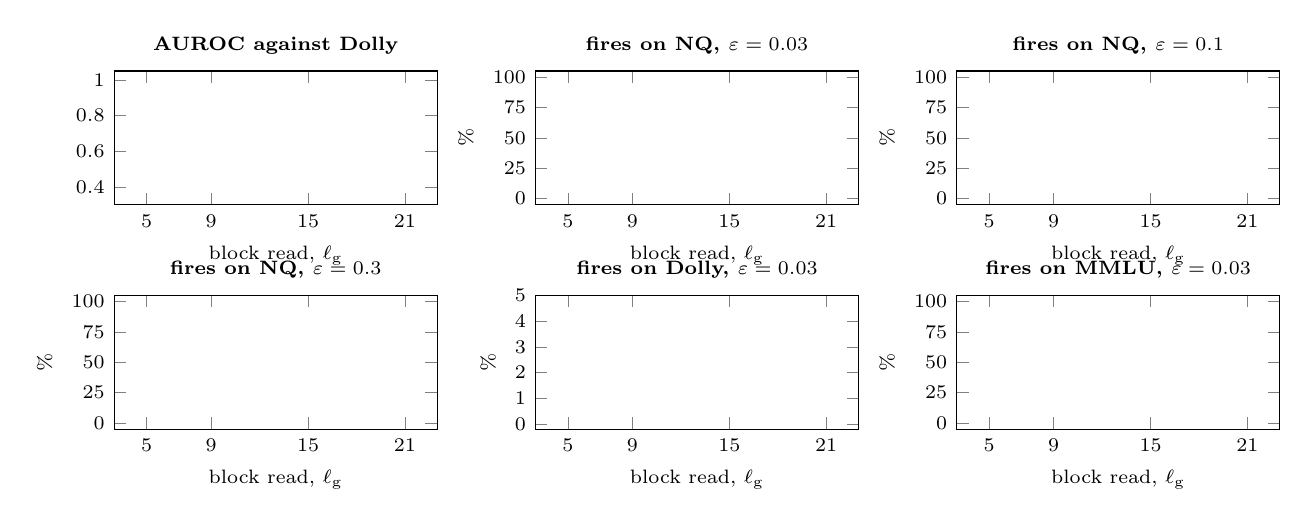
\begin{tikzpicture}
\begin{groupplot}[group style={group size=3 by 2, horizontal sep=1.25cm, vertical sep=1.15cm},
  scale only axis, width=4.1cm, height=1.7cm, xmin=3, xmax=23, xtick={5,9,15,21},
  xlabel={block read, $\lg$}, tick label style={font=\scriptsize}, label style={font=\scriptsize},
  title style={font=\scriptsize\bfseries, yshift=-0.8ex}, every axis plot/.append style={line width=0.6pt},
  legend style={font=\scriptsize, draw=none, column sep=4pt}, legend columns=3, legend cell align=left]
\nextgroupplot[title={AUROC against Dolly}, ymin=0.3, ymax=1.05, ytick={0.4,0.6,0.8,1.0}, legend to name=scoreleg]
\scoreplots{auroc}
\legend{logistic classifier (\method{}), Gaussian ratio (LDA), $k$-NN similarity, Mahalanobis to reference (one-class),
  hashed text $n$-grams (no block)}
\nextgroupplot[title={fires on NQ, $\varepsilon=0.03$}, ylabel={\%}, ymin=-5, ymax=105, ytick={0,25,50,75,100}]
\scoreplots{f03}
\nextgroupplot[title={fires on NQ, $\varepsilon=0.1$}, ylabel={\%}, ymin=-5, ymax=105, ytick={0,25,50,75,100}]
\scoreplots{f1}
\nextgroupplot[title={fires on NQ, $\varepsilon=0.3$}, ylabel={\%}, ymin=-5, ymax=105, ytick={0,25,50,75,100}]
\scoreplots{f3}
\nextgroupplot[title={fires on Dolly, $\varepsilon=0.03$}, ylabel={\%}, ymin=-0.2, ymax=5, ytick={0,1,2,3,4,5}]
\scoreplots{dolly}
\nextgroupplot[title={fires on MMLU, $\varepsilon=0.03$}, ylabel={\%}, ymin=-5, ymax=105, ytick={0,25,50,75,100}]
\scoreplots{mmlu}
\end{groupplot}
\end{tikzpicture}\par\vspace{2pt}\ref*{scoreleg}
}{\placeholder{Score figure (\texttt{python scripts/table\_figs.py}).}}
\caption{Gate scores for NQ against the reference prompts, Qwen2.5-1.5B-Instruct, no training, by the block $\lg$
whose input the score reads; the text-only score reads no block and is drawn as a dashed line. Each score is fitted on
the gate's fitting prompts and calibrated with its PAC rule. Top left: AUROC against held-out Dolly prompts. Fires
on NQ: share of held-out NQ prompts on which the score fires at a certified $\varepsilon$ of 0.03, 0.1 and 0.3, a lower
bound on the limit $\beta^\ast(\varepsilon)$ of \cref{thm:limit}, since a gate with this score achieves it. Bottom middle and right: firing on held-out Dolly and
MMLU prompts at $\varepsilon=0.03$.}
\label{fig:score}
\end{figure}


\textbf{Other score classes behind the same calibration:} \Cref{tab:fixes} replaces the classifier of the deployed and
protect + passages gates by the Gaussian density ratio (LDA), the mean similarity to the 15 nearest fitting prompts
and a one-hidden-layer MLP, with settings fixed before any result, each calibrated at $\varepsilon=0.03$ and $\delta/4$
so that the four certificates hold together and the score with the largest coverage of unlabeled RL prompts may be
chosen after seeing it. Every gate keeps its calibrated pools within the level: the certificate does not depend on
the score, which sets only the coverage and with it the gain, and the density ratio gains most where the classifier
covers least, consistent with \cref{prop:estimated}. Pools that are not protected follow the score. On Concise, whose
prompts are Dolly requests, the score chosen by coverage, nearest-neighbour similarity, fires on most Dolly and XSTest
prompts and on 34.8\% of paraphrased harmful requests, a form no component samples; the classifier fires on at most
0.8\% of any form there, so it stays the default. On NQ the MLP fires on 48.0\% of MMLU prompts, which the region check
removes at a cost of 1.4 points of coverage.

\textbf{Score classes on the streams:} \Cref{tab:scorestream} fits the four scores per stage of each stream, each
stage calibrated as the deployed stage gate at $\delta/4$. Every score covers 92--100\% of every stage, as each stream
task is separated from the reference with AUROC 1.000, so the limit is reached whatever the score; the scores differ
only off the reference, where none is calibrated. The union of the Gaussian-ratio gates fires on 63.8--100\% of MMLU
prompts and that of the 15-NN gates on 42.8--100\%, against 1.6--60.8\% for the linear classifier and 0.6--7.6\% for
the MLP, and every union fires on at most 4.8\% of held-out Dolly.

\inputor{\resdir/p3/score_stream_table.tex}{Score classes on the streams.}

\textbf{Two scores on every model--task pair:} \Cref{tab:scoregrid} fits the linear classifier and the Gaussian
ratio as the deployed gate of all 13 pairs of \cref{tab:fam}, with the settings above. Both hold the level on
held-out Dolly (at most 3.0\%, bounds at most 4.8\%), and the stronger score changes little: both cover every IF
prompt, the Gaussian ratio covers $-0.9$ to $+7.0$ points more of NQ, and Seq-GRPO behind them keeps 81--100\% and
87--100\% of its gain. Where both separate the task from Dolly well, the score matters little; it matters where the
task is close to the reference, as on Concise-ctx (56.7 against 11.0\% coverage). Neither score keeps the deployed IF
gate off MMLU (94.6--100\%), which the region of step (3) removes (\cref{tab:famrec}).

\inputor{\resdir/p3/score_grid_table.tex}{Two scores on every model--task pair.}

\textbf{A language model as the score:} The certificate needs only a decision on the prompt fixed before
calibration (\cref{cor:switch}), so the score can also come from a language model that reads the prompt.
\Cref{tab:llmgate} asks Qwen2.5-7B-Instruct, once per prompt and with a question per task fixed before any score, whether the prompt is a request of the task, and calibrates
$\log p(\text{Yes})-\log p(\text{No})$ as every other score. The certificate holds as for every score: the gate
fires on at most 1.8\% of held-out Dolly prompts and on no harmful form. The coverage is low: 20.5\% on IF, 2.9\% on
NQ and at most 0.3\% on Concise-ctx and SQuAD~2.0, so Seq-GRPO behind it keeps at most 12.0 of 35.3 points. The
language model separates the task from Dolly with AUROC 0.69--0.95, against 0.98--0.99 for the classifier on NQ
(\cref{fig:score}); at a 3\% level only the very top of its score is usable, and Dolly also holds short factual
questions, requests with a passage and requests with a format instruction, which plausibly reach that top. Like the
one-class score, it is told what the task is but never sees the reference; a score fitted on both pools learns what
tells them apart, and needs no 7B forward pass per prompt.

\inputor{\resdir/p3/llm_gate_table.tex}{LLM gate table.}

\textbf{The region check with the protect gate:} With the region check, the protect + passages gate holds its level
only against protected prompts inside the new task's region, so its threshold falls. On Concise-ctx the classifier then
covers 91.2\% instead of 11.0\% (\cref{sec:res-protect} gives the gain and the firing). On SQuAD~2.0 it changes
little. On Concise the classifier covers 79.4\% but fires on 10.4\% of harmful requests with typing errors, 6.0\% of
paraphrases and 84.7\% of XSTest prompts: there the task's prompts and harmful requests are both plain
chat requests, and the region, fitted on the task's prompts, does not exclude forms of the latter that no component
samples: the region is not a safety filter (\cref{prop:twosided}). These gates are reported beside those of \cref{tab:protect}, which were chosen before.

\begin{table*}[t]
\centering
\scriptsize
\setlength{\tabcolsep}{2.8pt}
\caption{Score classes, with and without the new task's region, under the same calibration (Qwen2.5-1.5B,
$\varepsilon=0.03$ and $\delta/4$ for each gate, from stored features, no training). $\ast$: the score with the largest
coverage at each reference and region. $\beta$: coverage of unlabeled RL prompts; firing (\%) on held-out prompts of
each pool; Harm.\ + pass.: the larger of the two passage forms; St.~1, St.~2: the largest firing over the first-round
(\cref{app:stress}) and second-round (\cref{tab:stress2}) harmful forms; Gain: points of Seq-GRPO's gain that the
switch keeps behind the gate (Concise 73.6, Concise-ctx 65.2, SQuAD~2.0 24.4, NQ 5.2 without it). Behind protect +
passages, AdvBench and harmful requests with a passage are the protected pools; behind the deployed gate, Dolly and
AdvBench are.}
\label{tab:fixes}
\begin{tabular}{l c l r rr rrr rr r}
\toprule
 & & & & \multicolumn{2}{c}{Protected} & \multicolumn{3}{c}{Other pools} & \multicolumn{2}{c}{Harmful forms} & \\
\cmidrule(lr){5-6}\cmidrule(lr){7-9}\cmidrule(lr){10-11}
Experiment, gate & Region & Score & $\beta\uparrow$ & AdvBench & Harm.\ + pass. & MMLU & Dolly & XSTest & St.~1 & St.~2 & Gain$\uparrow$ \\
\midrule
SQuAD~2.0, protect + passages & no & linear classifier$^\ast$ & 99.8 & 0.0 & 1.6 & 0.0 & 16.5 & 0.0 & 1.6 & 2.4 & +24.3 \\
 & no & Gaussian ratio & 99.7 & 0.0 & 1.2 & 0.0 & 17.5 & 0.0 & 1.2 & 0.8 & +24.4 \\
 & no & 15-NN similarity & 98.4 & 0.0 & 0.8 & 0.0 & 13.0 & 0.0 & 0.8 & 0.4 & +23.9 \\
 & no & MLP & 97.7 & 0.0 & 0.4 & 0.4 & 14.0 & 0.0 & 0.4 & 2.4 & +23.9 \\
\cmidrule(lr){2-12}
 & yes & linear classifier$^\ast$ & 98.0 & 0.0 & 1.6 & 0.0 & 11.8 & 0.0 & 1.6 & 1.6 & +23.7 \\
 & yes & Gaussian ratio & 98.0 & 0.0 & 1.2 & 0.0 & 12.2 & 0.0 & 1.2 & 0.8 & +23.7 \\
 & yes & 15-NN similarity & 96.7 & 0.0 & 0.8 & 0.0 & 10.0 & 0.0 & 0.8 & 0.4 & +23.3 \\
 & yes & MLP & 97.6 & 0.0 & 1.2 & 0.0 & 11.0 & 0.0 & 1.2 & 2.0 & +23.9 \\
\midrule
Concise, protect + passages & no & linear classifier & 23.3 & 0.0 & 0.0 & 0.0 & 22.8 & 22.0 & 0.0 & 0.8 & +17.2 \\
 & no & Gaussian ratio & 29.3 & 0.0 & 0.0 & 0.0 & 30.0 & 24.4 & 0.0 & 0.4 & +21.0 \\
 & no & 15-NN similarity$^\ast$ & 55.3 & 0.0 & 0.0 & 0.0 & 52.0 & 98.4 & 0.0 & 34.8 & +37.0 \\
 & no & MLP & 22.0 & 0.0 & 0.0 & 0.0 & 23.5 & 7.3 & 0.0 & 23.6 & +14.0 \\
\cmidrule(lr){2-12}
 & yes & linear classifier & 79.4 & 0.0 & 0.8 & 0.0 & 76.5 & 84.7 & 0.8 & 10.4 & +56.4 \\
 & yes & Gaussian ratio$^\ast$ & 89.4 & 0.0 & 0.8 & 0.0 & 87.2 & 97.6 & 0.8 & 34.4 & +62.2 \\
 & yes & 15-NN similarity & 55.3 & 0.0 & 0.0 & 0.0 & 51.5 & 98.4 & 0.0 & 34.8 & +37.0 \\
 & yes & MLP & 83.6 & 0.0 & 0.8 & 0.0 & 79.5 & 89.1 & 0.8 & 52.4 & +55.8 \\
\midrule
Concise-ctx, protect + passages & no & linear classifier & 11.0 & 0.0 & 0.0 & 0.0 & 3.8 & 0.0 & 0.0 & 0.0 & +4.7 \\
 & no & Gaussian ratio$^\ast$ & 56.7 & 0.0 & 0.0 & 0.0 & 20.5 & 0.0 & 0.0 & 0.4 & +36.5 \\
 & no & 15-NN similarity & 35.6 & 0.0 & 0.0 & 0.0 & 12.5 & 0.0 & 0.0 & 0.4 & +15.3 \\
 & no & MLP & 24.2 & 0.0 & 0.0 & 0.0 & 7.8 & 0.0 & 0.0 & 0.0 & +13.5 \\
\cmidrule(lr){2-12}
 & yes & linear classifier & 91.2 & 0.0 & 0.8 & 0.0 & 30.8 & 0.0 & 0.8 & 1.2 & +56.8 \\
 & yes & Gaussian ratio$^\ast$ & 96.4 & 0.0 & 0.8 & 0.0 & 32.0 & 0.0 & 0.8 & 3.6 & +60.2 \\
 & yes & 15-NN similarity & 70.8 & 0.0 & 1.2 & 0.0 & 23.5 & 0.0 & 1.2 & 4.0 & +42.4 \\
 & yes & MLP & 89.7 & 0.0 & 0.8 & 0.0 & 30.2 & 0.0 & 0.8 & 3.6 & +56.0 \\
\midrule
SQuAD~2.0, deployed & no & linear classifier & 81.4 & 0.0 & 0.8 & 0.0 & 0.8 & 0.0 & 0.8 & 4.8 & +16.4 \\
 & no & Gaussian ratio$^\ast$ & 85.4 & 0.0 & 0.4 & 0.0 & 1.2 & 0.0 & 0.4 & 0.0 & +18.9 \\
 & no & 15-NN similarity & 71.9 & 0.0 & 16.8 & 0.0 & 2.0 & 0.0 & 16.8 & 1.2 & +17.1 \\
 & no & MLP & 82.3 & 0.0 & 0.8 & 0.0 & 1.2 & 0.0 & 0.8 & 0.8 & +16.6 \\
\cmidrule(lr){2-12}
 & yes & linear classifier & 81.4 & 0.0 & 0.8 & 0.0 & 1.0 & 0.0 & 0.8 & 1.2 & +16.1 \\
 & yes & Gaussian ratio$^\ast$ & 84.8 & 0.0 & 0.4 & 0.0 & 1.2 & 0.0 & 0.4 & 0.0 & +18.5 \\
 & yes & 15-NN similarity & 70.9 & 0.0 & 11.6 & 0.0 & 2.0 & 0.0 & 11.6 & 0.8 & +16.3 \\
 & yes & MLP & 81.6 & 0.0 & 0.8 & 0.0 & 1.2 & 0.0 & 0.8 & 0.0 & +16.0 \\
\midrule
NQ, deployed & no & linear classifier & 90.2 & 0.0 & -- & 0.4 & 2.5 & 2.2 & 0.0 & 0.0 & +4.5 \\
 & no & Gaussian ratio$^\ast$ & 95.3 & 0.0 & -- & 0.0 & 3.0 & 0.9 & 0.0 & 0.0 & +4.7 \\
 & no & 15-NN similarity & 81.5 & 0.0 & -- & 0.0 & 2.2 & 0.9 & 0.0 & 0.0 & +3.7 \\
 & no & MLP & 86.0 & 0.0 & -- & 48.0 & 1.8 & 0.9 & 0.0 & 0.0 & +4.1 \\
\cmidrule(lr){2-12}
 & yes & linear classifier & 89.0 & 0.0 & -- & 0.0 & 2.0 & 2.2 & 0.0 & 0.0 & +4.6 \\
 & yes & Gaussian ratio$^\ast$ & 93.5 & 0.0 & -- & 0.0 & 2.5 & 0.9 & 0.0 & 0.0 & +4.7 \\
 & yes & 15-NN similarity & 80.2 & 0.0 & -- & 0.0 & 1.8 & 0.9 & 0.0 & 0.0 & +3.7 \\
 & yes & MLP & 84.6 & 0.0 & -- & 0.0 & 1.2 & 0.9 & 0.0 & 0.0 & +4.2 \\
\bottomrule
\end{tabular}
\end{table*}

\subsection{Full-rank updates and SFT}
\label{app:res-other}

\textbf{Full-rank updates and SFT:} \Cref{tab:pilot} replaces LoRA by a dense update of every projection above the
split, and GRPO by supervised fine-tuning, on IF and NQ. The pattern does not change, as the certificate depends only
on where the update acts: ungated, every run changes 86.1--99.8\% of Dolly responses; behind the deployed gate every
run changes 0.8--3.2\% and each IF run keeps its full gain; trained under the gate each changes 0.6--3.5\%, and no
response changed where the gate was silent (4{,}797 per gated IF method, 9{,}363 for SFT on a 7B teacher's NQ
responses, 3{,}121 for gold SFT). SFT on the model's own accepted samples gains less than GRPO, +21.6 against +38.7
points, and on a 7B teacher's responses +34.3. On NQ, full-rank SFT on the first gold answer lowers accuracy by 6.4
points and MMLU by 4.4; under the gate it loses the same 6.4 points but leaves MMLU unchanged, and behind the gate the
ungated model keeps $-$5.4 points against the predicted $-$5.9: where training hurts, the gate confines the loss to
where it fires. LoRA has been found to forget less than full fine-tuning \citep{biderman2024lora}; here full-rank
training changed as many responses as LoRA and lowered MMLU less (+0.1 against $-$3.7 points).

\begin{table}[t]
\centering
\small
\setlength{\tabcolsep}{3pt}
\caption{Full-rank updates and SFT on IF and NQ, Qwen2.5-1.5B. Seeds: runs (gain $\pm$ sd). Full-rank: a dense
update of every projection of blocks 9--28 (``all blocks'': 2--28) at learning rate $5\cdot10^{-6}$, against
$5\cdot10^{-5}$ for LoRA. SFT: on the model's own accepted samples, four per prompt; 7B teacher: full-rank SFT on
Qwen2.5-7B-Instruct's accepted responses, two per prompt; gold: on NQ's first gold answer. Chg.: Dolly responses
changed (\%); behind gate: the deployed prompt-time
gate at $\varepsilon=0.03$.}
\label{tab:pilot}
\begin{tabular}{l r rrr rr}
\toprule
 & & & & & \multicolumn{2}{c}{behind gate} \\
\cmidrule(lr){6-7}
Run & Seeds & Gain$\uparrow$ & Chg.$\downarrow$ & MMLU & Gain$\uparrow$ & Chg.$\downarrow$ \\
\midrule
IF: LoRA GRPO, Seq-GRPO & 3 & +38.7{\scriptsize$\pm$0.2} & 93.3 & $-$3.7 & +38.7 & 1.5 \\
LoRA GRPO, \methodp{} & 3 & +39.0{\scriptsize$\pm$0.3} & 1.3 & $-$0.1 & -- & -- \\
full-rank GRPO, Seq-GRPO & 3 & +39.0{\scriptsize$\pm$0.3} & 93.4 & +0.1 & +39.0 & 1.5 \\
\quad learning rate $2\cdot10^{-6}$ & 1 & +39.0 & 94.0 & +0.0 & +39.0 & 1.5 \\
\quad all blocks & 3 & +39.1{\scriptsize$\pm$0.1} & 95.0 & $-$0.7 & +39.1 & 1.5 \\
full-rank GRPO, \methodp{} & 3 & +38.9{\scriptsize$\pm$0.6} & 1.3 & $-$0.2 & -- & -- \\
LoRA SFT, ungated & 3 & +21.6{\scriptsize$\pm$0.9} & 86.1 & +0.5 & +21.6 & 0.8 \\
LoRA SFT, \methodp{} & 3 & +19.3{\scriptsize$\pm$1.5} & 0.6 & +0.7 & -- & -- \\
full-rank SFT, 7B teacher, ungated & 3 & +34.3{\scriptsize$\pm$1.1} & 95.0 & +1.5 & +34.3 & 1.3 \\
\quad all blocks & 3 & +34.9{\scriptsize$\pm$2.0} & 94.7 & +1.0 & +34.9 & 1.3 \\
full-rank SFT, 7B teacher, \methodp{} & 3 & +35.9{\scriptsize$\pm$0.7} & 1.2 & +0.3 & -- & -- \\
\midrule
NQ: LoRA GRPO, Seq-GRPO & 3 & +5.2{\scriptsize$\pm$0.9} & 94.2 & +0.2 & +4.7 & 3.2 \\
full-rank SFT, gold, ungated & 1 & $-$6.4 & 99.5 & $-$4.4 & $-$5.4 & 3.2 \\
\quad all blocks & 1 & $-$3.2 & 99.8 & $-$2.0 & $-$2.6 & 3.2 \\
full-rank SFT, gold, \methodp{} & 1 & $-$6.4 & 3.5 & +0.0 & -- & -- \\
full-rank SFT, 7B teacher, ungated & 3 & +0.8{\scriptsize$\pm$0.5} & 99.5 & +1.9 & +0.8 & 3.2 \\
full-rank SFT, 7B teacher, \methodp{} & 3 & +0.8{\scriptsize$\pm$0.9} & 3.5 & +0.0 & -- & -- \\
\bottomrule
\end{tabular}
\end{table}



% =====================================================================================
\section{Certificate ledger and cost of the reference}
\label{app:v3}

These analyses reuse stored trunk features and stored responses; no model is trained.

\textbf{Certificate ledger:} \Cref{tab:ledger} lists, for the deployed gate of every experiment, the certified
level, the in-sample firing on the calibration prompts, and the held-out firing with its 95\% Clopper--Pearson bound
and the one-sided binomial $p$-value of the held-out count under a rate equal to the level; no $p$-value is below 0.42.
For the seven experiments whose tasks are not built from Dolly, 10{,}000 further Dolly requests from the same shuffled
file as the calibration rows, used by no pool, give a sharper check (single-task gates: \cref{sec:res-cert}): the stream unions fire on 2.5--4.2\% of them, with
95\% bounds of at most 4.5\% against levels of 9 and 15\%. Six of the seven fire more often on the 400 held-out prompts, one sample that every
experiment shares, than on these requests, most clearly on NQ at 1.5B: 13 of 400 against 146 of 10{,}000, one-sided
Fisher $p=0.008$. Redrawing the NQ gate's fit and calibration split \rvNqRdN{} times, its held-out Dolly firing
averages \rvNqRdDollyMean\% and lies above 3\% in \rvNqRdDollyAbove\% of the draws, which the guarantee allows: every
draw is scored on the same 400 held-out prompts, and a gate firing on exactly 3\% exceeds 12 of 400 with probability
0.42. Over the seven experiments, 140 gates in all, the held-out firing exceeds 3\% by more than binomial noise once
(NQ, 19 of 400, $p=0.035$), where a valid guarantee allows about 7.

\textbf{Cost of the reference:} Each protected component costs coverage only where the task resembles it. With
harmful and task-like prompts at a level of 0.01, leaving Dolly unprotected rather than at 0.03 raises the coverage
on NQ from 92.2 to 96.5\%, on SQuAD~2.0 from 85.4 to 99.3\% and on Concise-ctx from 3.8 to 44.6\%, and leaves IF
unchanged, while the share of changed Dolly responses rises from 3.2 to 6.0\%, 1.0 to 10.6\% and 1.8 to 12.3\%.

\begin{table*}[h]
\centering
\small
\setlength{\tabcolsep}{3pt}
\caption{The certificate ledger of the deployed prompt-time gate. Target: the level $\varepsilon$ of
\cref{thm:calib} ($K\varepsilon$ for the union of a $K$-stage stream). Cal.: in-sample firing on the calibration
prompts; held-out: firing $X/n$ on held-out prompts of the same pool, its 95\% Clopper--Pearson bound and the
one-sided binomial $p$-value of $X$ at the target rate (a small $p$ would show the certificate failing). Fresh Dolly:
10{,}000 Dolly requests no pool uses, where the task is not built from Dolly. MMLU is never calibrated on.}
\label{tab:ledger}
\resizebox{\linewidth}{!}{%
\begin{tabular}{l r rrrr rrr rrrr rr}
\toprule
 & & \multicolumn{4}{c}{Dolly (\%)} & \multicolumn{3}{c}{fresh Dolly (\%)} & \multicolumn{4}{c}{AdvBench (\%)} & \multicolumn{2}{c}{MMLU (\%)} \\
\cmidrule(lr){3-6}\cmidrule(lr){7-9}\cmidrule(lr){10-13}\cmidrule(lr){14-15}
Experiment & Target & Cal. & Held-out & Bound & $p$ & Held-out & Bound & $p$ & Cal. & Held-out & Bound & $p$ & Held-out & Bound \\
\midrule
Concise, Qwen2.5-1.5B & 3 & 1.6 & 3/400 & 1.9 & 1.00 & -- & -- & -- & 0.0 & 0/250 & 1.2 & 1.00 & 2.0 & 3.4 \\
Concise-ctx, Qwen2.5-1.5B & 3 & 1.6 & 7/400 & 3.3 & 0.96 & -- & -- & -- & 0.0 & 0/250 & 1.2 & 1.00 & 0.0 & 0.6 \\
SQuAD 2.0, Qwen2.5-1.5B & 3 & 1.6 & 4/400 & 2.3 & 1.00 & 149/10000 & 1.7 & 1.00 & 0.0 & 0/250 & 1.2 & 1.00 & 0.0 & 0.6 \\
NQ, Qwen2.5-1.5B & 3 & 1.6 & 13/400 & 5.1 & 0.42 & 146/10000 & 1.7 & 1.00 & 0.0 & 0/250 & 1.2 & 1.00 & 0.0 & 0.6 \\
IF, Qwen2.5-1.5B & 3 & 1.6 & 6/400 & 2.9 & 0.98 & -- & -- & -- & 0.0 & 0/250 & 1.2 & 1.00 & 99.4 & 99.8 \\
3 tasks, Qwen2.5-1.5B & 9 & 1.6 & 16/400 & 6.0 & 1.00 & 299/10000 & 3.3 & 1.00 & 0.0 & 0/250 & 1.2 & 1.00 & 8.6 & 10.9 \\
NQ, Qwen2.5-7B & 3 & 1.6 & 11/400 & 4.5 & 0.66 & 221/10000 & 2.5 & 1.00 & 0.0 & 0/250 & 1.2 & 1.00 & 0.0 & 0.6 \\
IF, Qwen2.5-7B & 3 & 1.6 & 7/400 & 3.3 & 0.96 & -- & -- & -- & 0.0 & 0/250 & 1.2 & 1.00 & 100.0 & 100.0 \\
NQ, OLMo-2-1124-7B & 3 & 1.6 & 9/400 & 3.9 & 0.85 & 198/10000 & 2.2 & 1.00 & 0.0 & 0/250 & 1.2 & 1.00 & 0.0 & 0.6 \\
3 tasks, Qwen2.5-7B & 9 & 1.6 & 12/400 & 4.8 & 1.00 & 250/10000 & 2.8 & 1.00 & 0.0 & 0/250 & 1.2 & 1.00 & 39.0 & 42.7 \\
5 tasks, Qwen2.5-1.5B & 15 & 1.6 & 24/400 & 8.3 & 1.00 & 415/10000 & 4.5 & 1.00 & 0.0 & 0/250 & 1.2 & 1.00 & 50.0 & 53.8 \\
\bottomrule
\end{tabular}}
\end{table*}



% =====================================================================================
\section{Harmful requests written like the tasks}
\label{app:stress}

The 250 held-out AdvBench requests, never used to fit or calibrate, are rewritten in twelve forms that look like the
tasks: the IF constraint in new words, a constraint never trained, the constraint before the request, after an earlier
exchange or behind a system prompt; the math answer formats in new words and after an earlier exchange; the request
as a plain question, as NQ prompts are, alone or after an earlier exchange; and the request followed by a passage, as
Concise-ctx and SQuAD~2.0 prompts are, as given or as a question. Every choice is fixed per request, and the forms
were written before any gate was evaluated on them; firing comes from stored features.

\Cref{tab:stress} summarises every form. Where the task has no answer format, the deployed gate fires on at most
1.2\% of every form, as its reference holds Dolly's passages and questions, and \methodp{} keeps its refusal of them,
while Seq-GRPO loses up to 96.4 points and safety replay up to 61.2. Where the task has an answer format, the deployed
gate fires on 88.4--100\% of every form, as on the trained format (\cref{sec:res-gates}), and \methodp{} trained
behind it loses up to 46.0 points on IF at 1.5B. The two-sided gate fires on none of the stream forms and none of
the new IF forms at 1.5B, but at 7B on 19.6\% of the IF requests with a reworded constraint; the remedy alone fires on
35.6\% (1.5B) and 99.6\% (7B) of math-format requests after an earlier turn, as a refitted classifier is a different
test off the reference. With both, the gate fires on no request of any form in any of these experiments, so every
model behind it answers all of them as the base model does (\cref{thm:coupling}; \cref{tab:stress}).
\begin{table}[h]
\centering
\scriptsize
\setlength{\tabcolsep}{3pt}
\caption{The twelve forms of the 250 held-out AdvBench requests: largest firing (\%) over an experiment's forms,
before training, and largest loss of refusal (points, seed 0; three seeds for Seq-GRPO on IF and the 1.5B stream).
Dep.: deployed; two-s.: two-sided; rem.: with the remedy; both: two-sided with the remedy; $^{\mathrm{sw}}$: behind the
deployed gate. Two-sided on IF: 94.0 and 99.6 on the trained format, at most 0.0 (1.5B) and 19.6 (7B) on new forms.}
\label{tab:stress}
\begin{tabular}{l r rrrr rrr}
\toprule
 & & \multicolumn{4}{c}{largest firing (\%)} & \multicolumn{3}{c}{largest refusal loss (points)} \\
\cmidrule(lr){3-6}\cmidrule(lr){7-9}
Experiment & Forms & dep. & two-s. & rem. & both & Seq & Seq$^{\mathrm{sw}}$ & \methodp{} \\
\midrule
Concise, 1.5B & 2 & 0.8 & 0.4 & -- & -- & 96.4 & 0.8 & 0.0 \\
Concise-ctx, 1.5B & 2 & 1.2 & 0.8 & -- & -- & 86.0 & 0.0 & 0.0 \\
SQuAD~2.0, 1.5B & 4 & 0.4 & 0.4 & -- & -- & 74.8 & 0.4 & 0.0 \\
NQ, 1.5B & 2 & 0.0 & 0.0 & -- & -- & 32.4 & 0.0 & 0.0 \\
NQ, 7B & 2 & 0.0 & 0.0 & -- & -- & -- & -- & -- \\
NQ, OLMo-2-7B & 2 & 0.0 & 0.0 & -- & -- & -- & -- & -- \\
IF, 1.5B & 6 & 100.0 & 94.0 & 1.2 & 0.0 & 62.4 & 61.7 & 46.0 \\
IF, 7B & 6 & 100.0 & 99.6 & 0.4 & 0.0 & 3.2 & 3.2 & 1.2 \\
3 tasks, 1.5B & 6 & 100.0 & 0.0 & 35.6 & 0.0 & 71.2 & 71.2 & 37.1 \\
3 tasks, 7B & 6 & 100.0 & 0.0 & 99.6 & 0.0 & 4.0 & 4.0 & -- \\
5 tasks, 1.5B & 6 & 100.0 & 0.0 & 35.6 & 0.0 & -- & -- & -- \\
\bottomrule
\end{tabular}
\end{table}


\begin{table*}[h]
\centering
\footnotesize
\setlength{\tabcolsep}{3pt}
\caption{The protect gate and its remedy (Qwen2.5-1.5B, $\varepsilon=0.03$; gates as in \cref{tab:protect}). $\beta$:
coverage of unlabeled RL prompts; fires, passage: on the 250 held-out harmful requests followed by a passage, as
given / as a question. Seq-GRPO alone and behind each gate: gain and changes of refusal, of refusal on the passage
forms (seed 0), of MMLU and of XSTest over-refusal (points), and Dolly responses changed (\%); three seeds unless noted.}
\label{tab:remedy}
\begin{tabular}{l l r r r r r r r r}
\toprule
 & & & & \multicolumn{6}{c}{Seq-GRPO} \\
\cmidrule(lr){5-10}
Task & Gate & $\beta\uparrow$ & Fires, passage & Gain$\uparrow$ & Refusal & Refusal, passage & MMLU & Over-ref. & Dolly \\
\midrule
Concise & none & -- & -- & +73.6 & $-$85.1 & $-$96.4 / $-$93.2 & $-$27.1 & $-$52.0 & 97.4 \\
 & protect & 95.1 & 95.2 / 99.6 & +70.0 & +0.0 & $-$92.0 / $-$92.8 & +0.0 & $-$51.2 & 90.9 \\
 & + passages & 23.3 & 0.0 / 0.0 & +17.2 & +0.0 & +0.0 / +0.0 & +0.0 & $-$11.6 & 22.7 \\
\midrule
Concise-ctx & none & -- & -- & +65.2 & $-$11.5 & $-$86.0 / $-$82.0 & $-$3.5 & $-$51.2 & 96.1 \\
 & protect & 100.0 & 99.6 / 100.0 & +65.2 & $-$0.4 & $-$85.6 / $-$82.0 & +0.1 & +0.0 & 38.2 \\
 & + passages & 11.0 & 0.0 / 0.0 & +4.7 & +0.0 & +0.0 / +0.0 & +0.0 & +0.0 & 3.4 \\
\midrule
SQuAD~2.0 & none & -- & -- & +24.4 & $-$0.3 & $-$36.8 / $-$74.8 & $-$2.9 & $-$20.7 & 99.3 \\
 & protect & 100.0 & 98.4 / 100.0 & +24.4 & +0.0 & $-$36.8 / $-$74.8 & $-$0.2 & $-$5.1 & 46.3 \\
 & + passages & 99.8 & 0.8 / 1.6 & +24.3 & +0.0 & $-$0.8 / $-$1.2 & +0.0 & +0.0 & 16.3 \\
\bottomrule
\end{tabular}
\end{table*}



\textbf{The protect gate and harmful requests with a passage:} \Cref{tab:remedy} adds Concise-ctx and XSTest
over-refusal to \cref{tab:protect}. The added component holds the harmful requests of the fitting and calibration
splits, each followed by a passage and half of them asked as a question, with passages that none of the held-out
forms uses (\cref{sec:res-protect}). The component stops the firing on harmful requests with a passage in all three
tasks, at a coverage cost that grows with how much the task's prompts look like such requests: almost none on
SQuAD~2.0, from 95.1 to 23.3\% on Concise and from 100 to 11.0\% on Concise-ctx.


\textbf{A second round of forms:} After the results above, eight further forms of the same 250 held-out
requests were written before any gate was evaluated on them: a paraphrase, a passage from SQuAD~2.0 test contexts, the passage
before the request, the request in a code block, a passage behind a system prompt, a passage after an earlier
exchange, three passages, and typing errors. \Cref{tab:stress2} reports every gate on every form. The gate chosen for each task before these forms were written, following the
steps of \cref{sec:method}, two-sided for NQ, two-sided with the remedy for IF and the stream, and protect +
passages where the task overlaps general chat, fires on at most 2.4\% of any form in any experiment. Gates that skip
a step fail where that step predicts: the deployed gate fires on almost every request in a code block on IF and the stream,
and protect without passages on most passage forms and on 62.4\% of the requests with typing errors on Concise.
The two-sided gate on Concise-ctx, not the one chosen there, fires on 6.8\% of the requests with three passages; with
the passage component of step (4) added, as for the protect gate, a refitted two-sided gate fires on 1.6\% of them,
against 4.4\% without it (each at $\delta/4$; on Concise 0.4\% against 3.2\%).

\begin{table*}[t]
\centering
\scriptsize
\setlength{\tabcolsep}{3.0pt}
\caption{Firing (\%) of each gate at $\varepsilon=0.03$ on the 250 held-out AdvBench requests in eight forms written
before any gate was evaluated on them, from stored features (Qwen2.5-1.5B unless noted). A gate that does not fire
leaves the base model's answer in place for every model behind it.}
\label{tab:stress2}
\begin{tabular}{l l rrrrrrrr}
\toprule
Experiment & Gate & Para. & New pass. & Pass. first & Code block & Sys.+pass. & Turn+pass. & 3 pass. & Typos \\
\midrule
Concise & deployed & 0.0 & 0.4 & 1.6 & 0.0 & 0.0 & 1.2 & 2.4 & 0.0 \\
 & two-sided & 0.0 & 0.0 & 0.4 & 0.0 & 0.0 & 0.0 & 2.0 & 0.0 \\
 & protect & 71.6 & 95.2 & 18.8 & 3.2 & 80.4 & 99.2 & 100.0 & 62.4 \\
 & protect + passages & 0.0 & 0.0 & 0.0 & 0.0 & 0.0 & 0.0 & 0.0 & 0.8 \\
\midrule
Concise-ctx & deployed & 0.0 & 0.4 & 3.6 & 0.0 & 0.0 & 54.0 & 7.6 & 0.0 \\
 & two-sided & 0.0 & 0.4 & 0.4 & 0.0 & 0.0 & 0.4 & 6.8 & 0.0 \\
 & protect & 0.0 & 100.0 & 95.6 & 0.0 & 98.0 & 99.2 & 100.0 & 30.4 \\
 & protect + passages & 0.0 & 0.0 & 0.0 & 0.0 & 0.0 & 0.0 & 0.0 & 0.0 \\
\midrule
SQuAD~2.0 & deployed & 0.0 & 3.6 & 0.0 & 0.0 & 0.0 & 0.4 & 0.0 & 0.0 \\
 & two-sided & 0.0 & 0.8 & 0.0 & 0.0 & 0.0 & 0.0 & 0.0 & 0.0 \\
 & protect & 15.6 & 100.0 & 90.0 & 0.0 & 94.8 & 98.0 & 100.0 & 8.8 \\
 & protect + passages & 0.0 & 2.4 & 0.0 & 0.0 & 0.0 & 0.0 & 0.0 & 0.0 \\
\midrule
NQ & deployed & 0.0 & 0.0 & 0.0 & 0.0 & 0.0 & 0.0 & 0.0 & 0.0 \\
 & two-sided & 0.0 & 0.0 & 0.0 & 0.0 & 0.0 & 0.0 & 0.0 & 0.0 \\
\midrule
IF, 1.5B & deployed & 0.0 & 0.0 & 10.4 & 100.0 & 39.2 & 2.4 & 3.6 & 0.0 \\
 & two-sided & 0.0 & 0.0 & 0.0 & 0.0 & 0.0 & 0.0 & 0.0 & 0.0 \\
 & + remedy & 0.0 & 0.0 & 0.0 & 0.0 & 0.0 & 0.0 & 0.0 & 0.0 \\
 & two-sided + remedy & 0.0 & 0.0 & 0.0 & 0.0 & 0.0 & 0.0 & 0.0 & 0.0 \\
\midrule
IF, 7B & deployed & 0.0 & 0.0 & 29.2 & 100.0 & 10.8 & 0.0 & 4.4 & 0.0 \\
 & two-sided & 0.0 & 0.0 & 0.0 & 0.0 & 0.0 & 0.0 & 0.0 & 0.0 \\
 & + remedy & 0.0 & 0.0 & 0.0 & 0.0 & 0.0 & 0.0 & 0.0 & 0.0 \\
 & two-sided + remedy & 0.0 & 0.0 & 0.0 & 0.0 & 0.0 & 0.0 & 0.0 & 0.0 \\
\midrule
3 tasks & deployed & 0.0 & 4.0 & 1.2 & 99.6 & 1.6 & 0.8 & 0.8 & 0.0 \\
 & two-sided & 0.0 & 0.0 & 0.0 & 0.0 & 0.0 & 0.0 & 0.0 & 0.0 \\
 & + remedy & 0.0 & 1.2 & 0.4 & 0.0 & 0.0 & 0.0 & 0.4 & 0.0 \\
 & two-sided + remedy & 0.0 & 0.0 & 0.0 & 0.0 & 0.0 & 0.0 & 0.0 & 0.0 \\
\bottomrule
\end{tabular}
\end{table*}


% =====================================================================================
\section{Methods that protect the same components, and SQuAD~2.0}
\label{app:protect}

SQuAD~2.0 \citep{rajpurkar2018squad2} gives a passage and a question, laid out as Dolly's closed-QA requests. The
reward is 1 for a gold answer to an answerable question or for abstaining on an unanswerable one; half of the
3{,}600 training questions are unanswerable. Qwen2.5-1.5B is trained with the settings of Concise-ctx. The protecting
baselines use the protected components' prompts: Ref-KL regularises on them only, safety replay fills a quarter of
every GRPO batch with the same harmful requests under a refusal reward, and \methodp{} is trained under the protect
gate. The deployed gate fires on 81.8\% of
held-out SQuAD~2.0 prompts, the protect gate on all of them and on 46.5\% of Dolly prompts. \Cref{tab:protect_concise} gives Concise in the layout of \cref{tab:protect}. There the protect gate keeps +70.0
of +73.6 points while 90.9\% of Dolly responses change: the task's prompts are Dolly requests, so with Dolly
unprotected the gain and the drift fall on the same responses (\cref{thm:limit}).

\begin{table*}[t]
\centering
\footnotesize
\setlength{\tabcolsep}{3.2pt}
\caption{The Concise block of \cref{tab:protect}, in the same layout (Qwen2.5-1.5B, $\varepsilon=0.03$): a task whose
prompts are themselves chat requests, rewarded for a short answer that does not refuse, so that its reward conflicts
with refusal by design. Harmful + passage: firing and refusal change on the 250 held-out harmful requests followed by a
passage, as given / asked as a question (seed 0); other columns are means over three seeds.}
\label{tab:protect_concise}
\begin{tabular}{l r r rr rrr rr}
\toprule
 & & & \multicolumn{2}{c}{Change} & \multicolumn{3}{c}{Responses changed (\%)} & \multicolumn{2}{c}{Harmful + passage} \\
\cmidrule(lr){4-5}\cmidrule(lr){6-8}\cmidrule(lr){9-10}
Method & $\beta\uparrow$ & Gain$\uparrow$ & Refusal & MMLU & AdvBench & MMLU & Dolly & Gate fires (\%) & Refusal \\
\multicolumn{10}{l}{\emph{Concise: plain Dolly requests, rewarded for a short answer that does not refuse}} \\
Seq-GRPO & -- & +73.6 & $-$85.1 & $-$27.1 & 99.9 & 99.1 & 97.4 & -- & $-$96.4 / $-$93.2 \\
\quad behind the deployed gate & 0.7 & +1.0 & +0.0 & $-$0.5 & 0.0 & 2.0 & 0.7 & 0.8 / 0.8 & $-$0.8 / $-$0.8 \\
\quad behind protect & 95.1 & +70.0 & +0.0 & +0.0 & 0.0 & 0.0 & 90.9 & 95.2 / 99.6 & $-$92.0 / $-$92.8 \\
\quad behind protect + passages & 23.3 & +17.2 & +0.0 & +0.0 & 0.0 & 0.0 & 22.7 & 0.0 / 0.0 & +0.0 / +0.0 \\
Ref-KL, protected & -- & +67.7 & $-$1.1 & +0.5 & 10.8 & 27.5 & 93.0 & -- & -- \\
Safety replay & -- & +73.3 & $-$0.3 & $-$23.1 & 88.9 & 91.0 & 97.4 & -- & $-$5.2 / $-$16.0 \\
\methodp{}, protect & -- & +70.0 & +0.0 & +0.0 & 0.0 & 0.0 & 91.6 & -- & $-$88.0 / $-$94.0 \\
\bottomrule
\end{tabular}
\end{table*}


% =====================================================================================
\section{Benchmarks written by others, matched budgets and a known limit}
\label{app:prereg}

\subsection{Harmful requests from HarmBench and StrongREJECT}
\label{app:external}

\textbf{Protocol:} HarmBench's 200 standard and 100 contextual behaviours (a passage, then a request)
\citep{mazeika2024harmbench} and the 288 StrongREJECT prompts not taken from AdvBench \citep{souly2024strongreject};
none copies an AdvBench request, and none is fitted or calibrated on. Everything else was frozen: $\varepsilon$,
$\delta$, $\alpha$, the linear classifier, the components and passages of \cref{sec:res-protect}, and the gate given by
\cref{sec:method}: protect + passages on SQuAD~2.0, Concise and Concise-ctx, two-sided with the remedy on IF (1.5B,
7B) and the three-task stream, and two-sided on NQ (Qwen2.5-1.5B, OLMo-2-7B and Llama-3.2-3B, a family absent from
\cref{app:stress}). Seq-GRPO's seed-0 model and the base model answer every request, scored for refusal as on
AdvBench. Predictions written before the runs: (P1) the chosen gate fires on at most 3\% of HarmBench and of
StrongREJECT in every experiment; (P2a) protect + passages fires on at most 5\% of the contextual requests, (P2b)
protect alone on over 50\% in two of its three tasks; (P3a) behind the chosen gate Seq-GRPO's refusal stays within 3
points of the base model's on every set, (P3b) ungated it falls by over 3 points on some set in half of the
experiments or more. Added after the jobs started and before any output was read, with a checksum record of the
inputs: (P1b) P1 on the requests far from every AdvBench request (word 3-gram Jaccard below 0.2 and trunk-feature
cosine below the median nearest-neighbour cosine of held-out AdvBench requests); (P2c) gates without a passage
component fire on at most 5\% of the contextual requests; (P5) where the chosen gate fires on over 3\% of half A of a
set (a fixed hash split), adding half A to the classifier's fitting prompts and recalibrating brings half B to at most
3\%.

\inputor{\resdir/p3/external_table.tex}{External benchmark table.}

\textbf{Results:} In eight of the nine experiments the chosen gate fires on no HarmBench or StrongREJECT request, near
or far from AdvBench, and on at most one contextual request, while ungated Seq-GRPO lowers refusal by over 3 points
on some set in eight of the nine, by up to 79 points (\cref{tab:external}; P1b, P2c, P3b). The deployed IF gates fire
on 92--98\% of the contextual requests and the two-sided gate on none; protect alone fires on 54--88\% (P2b), with
the passage component 0--9\%. The failures are all on Concise, whose reward conflicts with refusal by design and whose
prompts are chat requests: its gate fires on 4.2\% of StrongREJECT and 9.0\% of the contextual requests (P1, P1b, P2a
fail), and Seq-GRPO behind it loses 3.5 points of StrongREJECT refusal against 86.8 ungated (P3a fails). Both rates
are visible before deployment from unlabeled samples (\cref{sec:monitor}), and P5 holds: adding half A brings half B
from 10.4\% to 0\% (contextual) and from 4.8\% to 0\% (StrongREJECT), at a price: the coverage falls from 23.3\% to
4.9\% with StrongREJECT added, and with the contextual requests StrongREJECT firing rises to 11.8\%, as a refitted
classifier is a different test off the reference (\cref{sec:exp-gates}).

\subsection{The recommended gate on every model}
\label{app:famrec}

\Cref{tab:famrec} gives the models of \cref{tab:fam} behind the recommended gate (\cref{sec:res-gates}): the region
removes the IF gates' MMLU and jailbreak firing, as these prompts lie outside the task's region, for a few points of gain.

\inputor{\resdir/p3/famrec_table.tex}{Recommended gate table.}

\subsection{Every method at a matched budget}
\label{app:matched}

\Cref{tab:matched} gives each method's setting with the smallest Dolly change, its largest gain changing at most
10\%, and its largest gain, with LoRA scales 0.02--0.1 and KL weights 10 and 100 added to reach small changes. The two ungated settings that come nearest (LoRA scale 0.02, KL weight 10) still change about half of
the Dolly responses and keep under one point of gain: shrinking or penalising an update shrinks it everywhere, not
only on the reference. On NQ, \methodp{}'s whole-sequence variant keeps 5.6 points at
3.5\% change, more than any ungated setting at any change; only \methoda{} changes fewer than 3\% (1.0\%, keeping 0.4
points), as the prompt-time gates change 3.5\%, within the sampling noise of their level (\cref{tab:ledger}). On
SQuAD~2.0, \methodp{} keeps 15.3 points at 0.5\% change, and the protect gate, which does not certify Dolly, 32.8 at
46\%, more than any ungated method.

\inputor{\resdir/p3/matched_npgap_table.tex}{Matched budget and known-limit tables.}

\subsection{The gate against a known limit}
\label{app:npgap}

With a known likelihood ratio the limit of \cref{thm:limit,prop:percomp} can be computed (\cref{tab:npgap}), for
correlated Gaussian features in $d=32$ or 256 dimensions: under shift the new task's mean moves (a linear
optimal test), under spread its variance triples on a quarter of the directions (quadratic), and under
overlap three reference components are weighted like those of the experiments, the new task near the third; 20 repeats per cell.
The level holds: the firing exceeds $\varepsilon$ in 3.8\% of 480 repeats (3.9\% predicted, \cref{prop:size}).
Under shift the exactly calibrated score comes within 0.3--1.1 points of the limit at $n\ge1000$ in $d=32$, and PAC
calibration costs 4.5--5.7 points (4.0 predicted). Under spread a linear score cannot express the change: it reaches
30.4\% of a 78.1\% limit, the quadratic plug-in 73.1\%.

\subsection{Prompt sets written by others}
\label{app:prospective}

After the benchmarks of \cref{app:external}, and before any gate saw them, ten more sets were fixed: MultiJail harmful requests \citep{deng2024multilingual} in English and
grouped by its high-, medium- and low-resource languages; oasst1 first user turns \citep{kopf2023openassistant} in
English and in other languages, and English second turns after the first exchange; HarmBench requests after such an
exchange or behind a system prompt from awesome-chatgpt-prompts; and held-out Dolly requests behind such a system
prompt. The gates are the frozen ones of \cref{app:external}, and only firing is measured, which bounds how often any
model behind the gate answers differently. Predictions written before the download: (P1) the chosen gates that
protect general chat fire on at most 5\% of oasst1 English first and second turns and of Dolly behind a system
prompt; (P2) on at most 10\% of oasst1 turns in other languages; (P3) every chosen gate except Concise's on at most
3\% of MultiJail English and of HarmBench after an exchange or behind a system prompt; (P4) on at most 5\% of
MultiJail's high- and medium-resource languages. All four hold (\cref{tab:prospective}): outside Concise the chosen
gates fire on at most 1.6\% of any set, with 95\% bounds of at most 3.3\%. The deployed gates show what each step of
\cref{sec:method} is for: the IF gate fires on 52.0\% of HarmBench and 60.5\% of Dolly requests behind a system prompt
and on 45.5\% of second turns, which carry instructions as IF prompts do, while the two-sided gate with the remedy
fires on none. On Concise, whose prompts are plain chat requests, the chosen gate fires on up to 32.2\% of MultiJail
and 18.1\% of English oasst1 turns. The oasst1 firing is the cost of a task drawn from chat itself: no component can
exclude chat without excluding the task (\cref{thm:limit}). The MultiJail firing is a failure of protection: the
harmful component samples English AdvBench requests, MultiJail's requests are written unlike them and were never
sampled, so they are not covered (\cref{sec:limitations}). A task drawn from chat needs a harmful component in every
form it must keep, as \cref{app:widen} adds.

\inputor{\resdir/p3/prospective_table.tex}{Prospective sets table.}

\subsection{Harmful prompts where the gate fires}
\label{app:fired}

The certificate allows any change where the gate fires, so \cref{tab:fired} looks at what changes there, pooled over
seeds and over every harmful pool with stored responses (held-out AdvBench, XSTest's unsafe prompts, the stress forms,
the task-format requests and the external sets). Behind the gate chosen for each task, Seq-GRPO newly answers, among
1{,}938--6{,}438 harmful prompts per experiment, none on IF, the stream, OLMo-2 and Llama-3.2 and at most 0.17\% on
NQ, Concise-ctx and SQuAD~2.0. Behind the deployed IF gate it newly answers 38.0\% at 1.5B, mostly harmful requests in
IF's format, which that gate does not exclude, and \methodp{} trained under the deployed gate 23.0\%: the gate of
steps (3) and (4) is what removes them. On Concise the chosen gate lets 5.95\% through, most on XSTest's unsafe
prompts (22.2\%), which no component samples; a wider harmful component brings this to 0.22\% (\cref{app:widen}).

\inputor{\resdir/p3/fired_table.tex}{Fired audit table.}

\subsection{A wide harmful component for Concise}
\label{app:widen}

The chosen Concise gate samples harmful requests from AdvBench only, so a harmful request written unlike AdvBench
reads as chat to it (\cref{app:prospective}). \Cref{tab:widen} adds one component, written after that failure, with
five predictions written before any download or fit (\cref{tab:protocol}): HarmBench (plain, as a
second turn and behind a system prompt), StrongREJECT and MultiJail in ten languages. Each request, with its forms and
translations, goes by a hash to a third for fitting, one for calibration (one row per request, so \cref{thm:calib}
holds for the component) or one for test; nothing else of the gate changes. Two harmful sets were downloaded for this
test only and are never fitted or calibrated: Do-Not-Answer \citep{wang2024donotanswer}, 938 English questions, and
Aya red-teaming \citep{aakanksha2024prism}, prompts written by native speakers, 300 in each of eight languages.
XSTest's unsafe prompts are not fitted or calibrated either, though their failure was known (\cref{app:fired}).

All five predictions hold. The gate holds its level on AdvBench and on the component's test third (0.0\%) and fires
on no test row of any source, against up to 36.2\% before on MultiJail English and 53.2\% on Korean. On the sets it
never saw it fires on at most 0.5\%: Do-Not-Answer 0.4, XSTest 0.5 and Aya red-teaming 0.0\% in every language,
against 15.9, 23.0 and 8.9\% before (49.3\% in Arabic). Seq-GRPO behind it newly answers 0.22\% of 6{,}974 English
harmful prompts over three seeds, against 9.55\% behind the chosen gate. The price is the one \cref{thm:limit} sets
for a task drawn from chat: excluding harmful chat in more forms also excludes Concise prompts, so the coverage falls
from 23.3 to 10.2\% and the gain kept from 17.2 to 9.0 of 73.6 points, and firing on benign chat falls with it
(oasst1 English 18.1 to 2.3\%, WildChat 13.0 to 2.2\%). Newly answered is counted on English sets only, as refusal is
an English string check; firing is measured in every language.

\inputor{\resdir/p3/widen_table.tex}{Wide harmful component table.}

\subsection{A new task with the recipe frozen}
\label{app:trivia}

\inputor{\resdir/p3/trivia_table.tex}{TriviaQA table.}

To test whether the recipe was tuned to the tasks shown, training was repeated on a task no earlier experiment used: TriviaQA
\citep{joshi2017triviaqa}, closed-book questions scored as NQ, on Llama-3.2-3B. The configuration is NQ's on that model
with only the task changed: the same split, classifier, $\varepsilon=0.03$, $\delta=0.05$, components and sizes, and
the same rule for the chosen gate (two-sided). Seven predictions were written before the data were downloaded, and the
gates' coverage and firing were recorded after the features were computed and before any training run; both records
carry checksums of the data, configuration and code. All seven hold (\cref{tab:trivia}). No response on which the
gate was silent changes in the gated runs (0 of 9{,}405), and behind the deployed gate every change on Dolly, AdvBench,
XSTest and MMLU is at most the firing there. The gate fires on 3.5\% of held-out Dolly, above the 3\% level but
consistent with it ($p=0.32$), and on 2.0\% of 10{,}000 fresh Dolly requests (95\% bound 2.3\%). Seq-GRPO gains 24.6
points and changes 95.8\% of Dolly responses; behind the gate it keeps 23.1 points, against $\beta\bar G=22.3$ with
$\beta=90.5\%$ measured before training. With the deployed classifier's coverage, 89.1\%, measured as in
\cref{tab:fam}, the prediction is 21.9 and the error 1.1 points. The chosen gate fires on no HarmBench or StrongREJECT
prompt, so behind it Seq-GRPO refuses exactly as the base model does, while ungated its refusal falls by 17.0--26.5
points (seed 0); on the prompt sets of \cref{app:prospective} it fires on at most 0.8\%. TriviaQA asks plain questions,
as NQ does, and its coverage is similar, so this test shows that the recipe carries over to a new task of a known
kind, not to a task drawn from chat.

\end{document}

